%%%%%%%%%%%%%%%%%%%%%%%%%%%%%%%%%%%%%%%%%%%%%%%%%%%
%
%  New template code for TAMU Theses and Dissertations starting Fall 2016.  
%
%
%  Author: Sean Zachary Roberson
%  Version 3.16.10
%  Last Updated: 9/29/2016
%
%%%%%%%%%%%%%%%%%%%%%%%%%%%%%%%%%%%%%%%%%%%%%%%%%%%

\documentclass[12pt]{report}

%These next lines change the font. Fixes for certain
%fonts will be implemented in a future release.

%Comment this line if you do not wish to use Times
%New Roman. The font used will then be the LaTeX
%default of Computer Modern.
\usepackage{times}
%\usepackage{cmbright}
\usepackage[T1]{fontenc}

%Do not change these settings. The geometry package
%Adjusts the margins to those specified by the Thesis
%Manual. 
\usepackage[letterpaper]{geometry}
\geometry{verbose,tmargin=1.25in,bmargin=1.25in,lmargin=1.4in,rmargin=1.15in}
 \usepackage[doublespacing]{setspace}
 \usepackage{tocloft}
 \usepackage[rm, tiny, center, compact]{titlesec}
 \usepackage{indentfirst}
 \usepackage{etoolbox}

\usepackage{tocvsec2}
 \usepackage[titletoc]{appendix}
 \usepackage{appendix}
 \usepackage{tamuconfig}

\usepackage{rotating}

%These are common AMS packages. Many LaTeX documents
%have these packages declared in their preambles.
\usepackage{amsmath, amsthm}

%This package allows for the use of graphics in the
%document.
\usepackage{graphicx}

%If you have JPEG format images, add .jpg as an
%allowed file extension below. Same for Bitmaps (.bmp).
\DeclareGraphicsExtensions{.png}

%It is best practice to keep all your pictures in
%one folder inside the main directory in which your
%TeX file is kept. Here the folder is named "graphic."
%Replace the name here with your folder's name, if needed.
%The period is needed due to relative referencing.
\graphicspath{ {./graphic/} }

%If needed, this will allow you to add the word "Page"
%to extra pages on your front matter lists.
\usepackage{afterpage}

%This is from the mdwtools package; it fixes some
%footnote commands and allows you to have footnotes in
%tables via the savenotes environment.
\usepackage{footnote}


% Added to fix issues with pdf searching in some versions of LaTeX
%\usepackage[T1]{fontenc}\usepackage{lmodern}
%%%%%%%%%%%%%%%%%%%%%%%%%%%%%

% Hyperref setup below.  You should be able to get away with using uncommenting just the first line.
%\usepackage[hidelinks]{hyperref}

% if \usepackage[hidelinks]{hyperref} doesn't work try this.
% \usepackage{hyperref}  % Hidelinks is an option that removes link visiability.  TAMU Thesis Offices prefers to not see the links. But often doesn't work.  
% 
% \hypersetup{
%     colorlinks=true,
%     linkcolor=black,
%     citecolor=black,
%     filecolor=black,
%     urlcolor=black,
% }
%%%%%%%  End of hyperref setup.  One of these two options should work, but my motto with hyperref is when in doubt, comment it out!
%%%%%%%%%  This hopefully fixes the problem with vertical spacing of section headings at the top of the page..  Commented out in 1.0.7
% \preto\section{%
% \ifnum\value{section}>0\addtocontents{toc}{\vskip-6pt}\fi
% }
% \preto\subsection{%
% \ifnum\value{subsection}=0\addtocontents{toc}{\vskip-6pt}\fi
% \ifnum\value{subsection}>0\addtocontents{toc}{\vskip-6pt}\fi
% } 
%%%%%%%%%%%%%%%%%%%%%%%%%%%%%%%%%%%%%%%%%%%%%%%%%%%%%%

%\usepackage{color}
\usepackage{subcaption}
\usepackage{listings}
\usepackage{tikz}
%\usepackage{enumitem}
\usepackage[htt]{hyphenat}
\usepackage{longtable}

\setlength\parindent{24pt}

%  new definitions
\renewcommand{\div}{\bs{\nabla}\! \cdot \!}
\newcommand{\grad}{\bs{\nabla}}
\newcommand{\norm}[1]{\left\lVert#1\right\rVert_{L^2}}
\newcommand{\rattlesnake}{Rattlesnake }
% extra space
\newcommand{\qq}{\quad\quad}
% common reference commands
\newcommand{\eqt}[1]{Equation~\eqref{#1}}					% equation
\newcommand{\eqts}[2]{Equations~\eqref{#1}~and~\eqref{#2}}	% two equations
\newcommand{\eqtss}[2]{Equations~\eqref{#1}~-~\eqref{#2}}	% multiple equations
\newcommand{\fig}[1]{Figure~\ref{#1}}						% figure
\newcommand{\figs}[2]{Figures~\ref{#1}~and~\ref{#2}}		% two figures
\newcommand{\figss}[2]{Figures~\ref{#1}~-~\ref{#2}}			% multiple figures
\newcommand{\tbl}[1]{Table~\ref{#1}}						% table
\newcommand{\chpt}[1]{Chapter~\ref{#1}}						% section
\newcommand{\sct}[1]{Section~\ref{#1}}						% section
\newcommand{\app}[1]{Appendix~\ref{#1}}						% appendix

\newcommand{\bs}[1]{\mathbf{#1}}
\newcommand{\dd}{\mathrm{d}}
\newcommand{\keff}{k_\textit{eff}}

\newcommand{\be}{\begin{equation}}
\newcommand{\ee}{\end{equation}}
\newcommand{\vn}{\vec{n}}
\newcommand{\vel}{\vec{\mathrm{v}}}
\newcommand{\adj}{\Phi^\dagger_0}
\newcommand{\FiguresDir}{./figures}

\definecolor{britishracinggreen}{rgb}{0.0, 0.26, 0.15}
\newcommand{\tcr}[1]{\textcolor{red}{#1}}
\newcommand{\tcb}[1]{\textcolor{blue}{#1}}
\newcommand{\tcm}[1]{\textcolor{magenta}{#1}}
\newcommand{\tcp}[1]{\textcolor{violet}{#1}}
\newcommand{\tcg}[1]{\textcolor{britishracinggreen}{#1}}

% tikz stuff
\usetikzlibrary{shapes,arrows,positioning}
\pgfdeclarelayer{background}
\pgfdeclarelayer{foreground}
\pgfsetlayers{background,main,foreground}
\tikzstyle{redblock}=[rectangle, draw, align=center, top color=red!25, bottom color=red!75,  minimum width=10mm, minimum height=10mm,]
\tikzstyle{blueblock}=[rectangle,draw, align=center, top color=blue!25, bottom color=blue!75,  minimum width=10mm, minimum height=10mm]
\tikzstyle{purpleblock}=[rectangle,  draw, align=center, top color=purple!25, bottom color=purple!75, minimum width=10mm, minimum height=10mm]
\tikzstyle{orangeblock}=[rectangle, draw, align=center, top color=orange!25, bottom color=orange!75,  minimum width=10mm, minimum height=10mm]
\tikzstyle{greendiamond}=[diamond, draw, align=center, top color=green!25, bottom color=green!75,  minimum width=8mm, aspect=2]
\tikzstyle{greenblock}=[rectangle, rounded corners, draw, align=center, top color=white, bottom color=green!20, ultra thick, minimum width=60mm, minimum height=15mm,]
\tikzstyle{blueblock2}=[rectangle, rounded corners, draw, align=center, top color=white, bottom color=blue!20, ultra thick, minimum width=60mm, minimum height=15mm]
\tikzstyle{reddiamond}=[diamond, draw, align=center, top color=white, bottom color=red!20, ultra thick, minimum width=60mm, aspect=2]
\newcommand{\tikzback}[5]{
 \begin{pgfonlayer}{background}
  \path (#1.west |- #2.north)+(-0.5,0.75) node (a1) {};
  \path (#3.east |- #4.south)+(+0.5,-0.25) node (a2) {};
  \path[fill=yellow!10,rounded corners, draw=black!100, dashed] (a1) rectangle (a2);
   \path (#3.east |- #2.north)+(0,1.25)--(#1.west |- #2.north) node[midway] (#5-n) {};
   \path (#3.east |- #2.south)+(0,-0.35)--(#1.west |- #2.south) node[midway] (#5-s) {};
   \path (#1.west |- #2.north)+(-0.75,0)--(#1.west |- #4.south) node[midway] (#5-w) {};
 \end{pgfonlayer}}
 
 % input stuff
\lstset{%
%  language=C++,
  showstringspaces=false,
  basicstyle=\footnotesize\ttfamily,
  commentstyle=\color{inl@green},
  frame=single,
  lineskip={-1.5pt}
}

%%%%%%%%%%%%%%%%%%%%%%%%%%%%%%%%%%%%%%%%%%%%%%%%%%%%%%

\begin{document}

%The title of your document goes here.
%Spacing may need to be adjusted if your title is long
%and pushes the copyright off the page.
\renewcommand{\tamumanuscripttitle}{Improved Quasi-Static Methods for Time-Dependent Neutron Diffusion and Implementation in Rattlesnake}

%Type only Thesis, Dissertation, or Record of Study.
\renewcommand{\tamupapertype}{Thesis}

%Your full name goes here, as it is in university records. Check your student record on Howdy if there is any mismatch.
\renewcommand{\tamufullname}{Zachary M. Prince}

%The degree title goes here. See the OGAPS site for more info.
\renewcommand{\tamudegree}{Master of Science}
\renewcommand{\tamuchairone}{Dr. Jean C. Ragusa}
\renewcommand{\tamumemberone}{Dr. Jim E. Morel}
\newcommand{\tamumembertwo}{Dr. Bojan Popov}
\renewcommand{\tamudepthead}{Dr. Yassin Hassan}

%Type only May, August, or December.
\renewcommand{\tamugradmonth}{May}
\renewcommand{\tamugradyear}{2017}
%Your department name goes here.
\renewcommand{\tamudepartment}{Nuclear Engineering}


%%%%%%%%%%%%%%%%%%%%%%%%%%%%%%%%%%%%%%%%%%%%%%%%%%%
%
%  New template code for TAMU Theses and Dissertations starting Fall 2016.  
%
%
%  Author: Sean Zachary Roberson
%	 Version 3.16.09
%  Last updated 9/12/2016
%
%%%%%%%%%%%%%%%%%%%%%%%%%%%%%%%%%%%%%%%%%%%%%%%%%%%

%%%%%%%%%%%%%%%%%%%%%%%%%%%%%% 
%% TITLE PAGE
%% The values get updated automatically.  Please do not make changes to this file other than adding/deleting committee members where necessary.
%%%%%%%%%%%%%%%%%%%%%%%%%%%%%%

\providecommand{\tabularnewline}{\\}



\begin{titlepage}
\begin{center}
\MakeUppercase{\tamumanuscripttitle}
\vspace{4em}

A \tamupapertype

by

\MakeUppercase{\tamufullname}

\vspace{4em}

\begin{singlespace}

Submitted to the Office of Graduate and Professional Studies of \\
Texas A\&M University \\

in partial fulfillment of the requirements for the degree of \\
\end{singlespace}

\MakeUppercase{\tamudegree}
\par\end{center}
\vspace{2em}
\begin{singlespace}
\begin{tabular}{ll}
 & \tabularnewline
& \cr
% If you have Co-Chairs comment out the 'Chair of Committee' line below and uncomment the 'Co-Chairs of Committee' line.
Chair of Committee, & \tamuchairone\tabularnewline
%Co-Chairs of Committee, & \tamuchairone\tabularnewline & \tamuchairtwo\tabularnewline
Committee Members, & \tamumemberone\tabularnewline
 & \tamumembertwo\tabularnewline
% & \tamumemberthree\tabularnewline
Head of Department, & \tamudepthead\tabularnewline

\end{tabular}
\end{singlespace}
\vspace{3em}

\begin{center}
\tamugradmonth \hspace{2pt} \tamugradyear

\vspace{3em}

Major Subject: \tamudepartment \par
\vspace{3em}
Copyright \tamugradyear \hspace{.5em}\tamufullname 
\par\end{center}
\end{titlepage}
\pagebreak{}




 % This is simply a file that formats and adds your titlepage, please do not edit this unless you have a specific need. .
%%%%%%%%%%%%%%%%%%%%%%%%%%%%%%%%%%%%%%%%%%%%%%%%%%%
%
%  New template code for TAMU Theses and Dissertations starting Fall 2016.  
%
%  Author: Sean Zachary Roberson
%	 Version 3.16.09
%  Last updated 9/12/2016
%
%%%%%%%%%%%%%%%%%%%%%%%%%%%%%%%%%%%%%%%%%%%%%%%%%%%
%%%%%%%%%%%%%%%%%%%%%%%%%%%%%%%%%%%%%%%%%%%%%%%%%%%%%%%%%%%%%%%%%%%%%
%%                           ABSTRACT 
%%%%%%%%%%%%%%%%%%%%%%%%%%%%%%%%%%%%%%%%%%%%%%%%%%%%%%%%%%%%%%%%%%%%%

\chapter*{ABSTRACT}
\addcontentsline{toc}{chapter}{ABSTRACT} % Needs to be set to part, so the TOC doesnt add 'CHAPTER ' prefix in the TOC.

\pagestyle{plain} % No headers, just page numbers
\pagenumbering{roman} % Roman numerals
\setcounter{page}{2}

\indent Transient reactor simulations are a chronically formidable challenge due to the computational rigor of evaluating the neutron transport equation, as well as its coupling with other physical phenomena. The goal of this thesis research is to mitigate the computational expense of these simulations by investigating and developing the improved quasi-static method (IQS). IQS is a rigorous space/time multiscale approach whereby the neutron flux is represented by a time-dependent amplitude and a time-space-energy dependent shape.  The objective of the IQS factorization is to evaluate amplitude and shape on different time scales in order to reduce computational burden associated with solving the multi-dimensional flux equations, while maintaining solution accuracy. IQS factorization leads to a nonlinear system of equations that requires iteration of shape and amplitude. Furthermore, reactor simulations often require coupling to additional multiphysics components for temperature feedback. These additional physics may evolve on different time scales and the applicability of IQS in multiphysic simulations needs to be evaluated from this perspective as well.

The objectives of this research is to establish IQS performance with various iteration techniques, validate time step convergence of IQS, and apply IQS to multiphysics simulation. IQS iteration techniques involve fixed-point (Picard) iteration with various convergence criteria and Newton iteration, namely preconditioned Jacobian-free Newton Krylov (PJFNK) method. Nonlinear convergence of each of these techniques is investigated. Validation of IQS with analysis of time step convergence is vital for implementation of time adaptive methods and error prediction. The time derivative of the shape function is discretized through fourth order using implicit-Euler, Crank-Nicolson, backward difference formulae (BDF), and singly-diagonally-implicit Runge-Kutta (SDIRK) methods. IQS application to multiphysics simulations involves its implementation into the Rattlesnake/MOOSE framework. These simulations allow insight to the performance of IQS for full transient reactor simulations.

The results of the iteration convergence analysis show that the most rigorous and comprehensive iteration technique is fixed-point iteration with consistency in the IQS uniqueness specification as the convergence criteria. This iteration technique revealed the need for analytical treatment of the precursor equation for proper convergence. For time step convergence analysis, IQS was applied to a one-dimensional prototype example, as well as the TWIGL and LRA benchmark.  The prototype results show that IQS has proper error convergence through fourth order discretization schemes. The TWIGL and LRA benchmark results show that IQS has proper convergence for implicit Euler, second-order BDF, and Crank-Nicolson schemes, validating IQS for more complex problems. For multiphysics simulation, IQS was applied to the LRA benchmark and a full core TREAT model. The results show that integration of temperature into the quasi-static process made considerable improvement to IQS performance. These results and conclusions helped gain insight into the behavior of IQS and furthered its development in complete transient reactor models.


 

\pagebreak{}

%%%%%%%%%%%%%%%%%%%%%%%%%%%%%%%%%%%%%%%%%%%%%%%%%%%
%
%  New template code for TAMU Theses and Dissertations starting Fall 2016.  
%
%  Author: Sean Zachary Roberson
%	 Version 3.16.09
%  Last updated 9/12/2016
%
%%%%%%%%%%%%%%%%%%%%%%%%%%%%%%%%%%%%%%%%%%%%%%%%%%%

%%%%%%%%%%%%%%%%%%%%%%%%%%%%%%%%%%%%%%%%%%%%%%%%%%%%%%%%%%%%%%%%%%%%%%
%%                           DEDICATION
%%%%%%%%%%%%%%%%%%%%%%%%%%%%%%%%%%%%%%%%%%%%%%%%%%%%%%%%%%%%%%%%%%%%%
\chapter*{DEDICATION}
\addcontentsline{toc}{chapter}{DEDICATION}  % Needs to be set to part, so the TOC doesnt add 'CHAPTER ' prefix in the TOC.



\begin{center}
\vspace*{\fill}
To my mother, my father, my grandmother, and my grandfather.
\vspace*{\fill}
\end{center}

\pagebreak{}

%%%%%%%%%%%%%%%%%%%%%%%%%%%%%%%%%%%%%%%%%%%%%%%%%%%%
%
%  New template code for TAMU Theses and Dissertations starting Fall 2016.
%
%  Author: Sean Zachary Roberson
%	 Version 3.16.09
%  Last updated 9/12/2016
%
%%%%%%%%%%%%%%%%%%%%%%%%%%%%%%%%%%%%%%%%%%%%%%%%%%%


%%%%%%%%%%%%%%%%%%%%%%%%%%%%%%%%%%%%%%%%%%%%%%%%%%%%%%%%%%%%%%%%%%%%%%
%%                           ACKNOWLEDGMENTS
%%%%%%%%%%%%%%%%%%%%%%%%%%%%%%%%%%%%%%%%%%%%%%%%%%%%%%%%%%%%%%%%%%%%%
\chapter*{ACKNOWLEDGMENTS}
\addcontentsline{toc}{chapter}{ACKNOWLEDGMENTS}  % Needs to be set to part, so the TOC doesnt add 'CHAPTER ' prefix in the TOC.


\indent This section is also optional, limited to four pages. It must follow the Dedication Page (or Abstract, if no Dedication). If listing preliminary pages in Table of Contents, include Acknowledgments. Heading (\MakeUppercase{Acknowledgments}) is bold if major headings are bold. It should be in same type size and style as text. So does vertical spacing, paragraph style, and margins. Also, ensure that the spelling of ``acknowledgments'' matches throughout the text and the table of contents.

I would like to thank the Texas A\&M University Office of Graduate and Professional Studies to allow me to construct this \LaTeX\ thesis template. Special thanks to JaeCee Crawford, Amy Motquin, Ashley Schmitt, Rachel Krolczyk, and Roberta Caton for carefully reviewing this material.  % use A\&M instead of A$\&$M, not use $A\&M$ as well, the last one won't be bold.



\pagebreak{}
%%%%%%%%%%%%%%%%%%%%%%%%%%%%%%%%%%%%%%%%%%%%%%%%%%%
%
%  New template code for TAMU Theses and Dissertations starting Fall 2016.  
%
%
%  Author: Sean Zachary Roberson
%	 Version 3.16.09 
%  Last updated 9/12/2016
%
%%%%%%%%%%%%%%%%%%%%%%%%%%%%%%%%%%%%%%%%%%%%%%%%%%%


%%%%%%%%%%%%%%%%%%%%%%%%%%%%%%%%%%%%%%%%%%%%%%%%%%%%%%%%%%%%%%%%%%%%%%
%%             CONTRIBUTORS AND FUNDING SOURCES
%%%%%%%%%%%%%%%%%%%%%%%%%%%%%%%%%%%%%%%%%%%%%%%%%%%%%%%%%%%%%%%%%%%%%
\chapter*{CONTRIBUTORS AND FUNDING SOURCES}
\addcontentsline{toc}{chapter}{CONTRIBUTORS AND FUNDING SOURCES}  % Needs to be set to part, so the TOC doesn't add 'CHAPTER ' prefix in the TOC.


%This section is taken directly from the MS Word templates.

%Old version below.

%All theses and dissertations must include a contributors and funding sources section. In this section, name all members of the dissertation committee, and any collaboration with others in carrying out your thesis or dissertation research. Your independent contributions must be made clear.
%
%If financial support from the university or any other source was gained to conduct your thesis or dissertation research and compilation, it must be listed in this section. If you completed all work independently without outside financial support, indicate this here.
%\textit{(Sample Wording)}
%
%This work was supported by a dissertation committee consisting of Professor XXX [advisor – also note if co-advisor] and XXXX of the Department of [Home Department] and Professor(s) XXXX of the Department of [Outside Department].
% 
%The data analyzed for Chapter III was provided by Professor XXXX. The analyses depicted in Chapter IV were conducted in part by Rebecca Jones of the Department of Biostatistics and were published in (year) in an article listed in the Biographical Sketch. 
%
%All other work conducted for the dissertation was completed by the student independently.
%
%\noindent \textit{(or)}
%
%This work was supervised by a dissertation committee consisting of Professor XXXX [advisor – also note if co-advisor] and Professor(s) XXXX of the Department of [Home Department] and Professor(s) XXXX of [Outside Department]. All work for the dissertation was completed independently by the student.
%
%\noindent \textit{(or)}
%
%Graduate study was supported by a fellowship from Texas A\&M University and a dissertation research fellowship from XXX Foundation.

\subsection*{Contributors}
This work was supported by a thesis committee consisting of Professors Jean Ragusa and Jim Morel of the Department of Nuclear Engineering and Professor Bojan Popov of the Department of Mathematics.

All other work conducted for the thesis was completed by the student independently with the direction of his adviser Dr. Jean Ragusa.
\subsection*{Funding Sources}
Graduate study was supported by the Endowed Doctoral Fellowship from Texas A\&M University, Idaho National Laboratory, and Integrated University Program Fellowship from the Department of Energy. 
\pagebreak{}
%%%%%%%%%%%%%%%%%%%%%%%%%%%%%%%%%%%%%%%%%%%%%%%%%%%
%
%  New template code for TAMU Theses and Dissertations starting Fall 2016.
%
%
%  Author: Sean Zachary Roberson
%	 Version 3.16.09
%  Last updated 9/12/2016
%
%%%%%%%%%%%%%%%%%%%%%%%%%%%%%%%%%%%%%%%%%%%%%%%%%%%

%%%%%%%%%%%%%%%%%%%%%%%%%%%%%%%%%%%%%%%%%%%%%%%%%%%%%%%%%%%%%%%%%%%%%%
%%                           NOMENCLATURE
%%%%%%%%%%%%%%%%%%%%%%%%%%%%%%%%%%%%%%%%%%%%%%%%%%%%%%%%%%%%%%%%%%%%%

\chapter*{NOMENCLATURE}
\addcontentsline{toc}{chapter}{NOMENCLATURE}  % Needs to be set to part, so the TOC doesnt add 'CHAPTER ' prefix in the TOC.

%A note about aligning: These entries will align
%themselves according to the ampersand (&).
%No extra spaces are needed, as seen in some of
%the entries below.
\vspace{-0.5in}
	\begin{table}[htbp]
	    \begin{tabular}{@{}p{0.25\textwidth} p{0.74\textwidth}@{}}
		IQS 	& 	Improved Quasi-Static Method\\ & \\
		INL 	& 	Idaho National Laboratory\\ & \\
		MOOSE 	& 	Multiphysics Object-Oriented Simulation Environment\\ & \\
		DOE 	& 	Department of Energy\\ & \\  
		NEAMS 	& 	Nuclear Energy Advanced Modeling and Simulation\\ & \\  
		PRKE 	& 	Point Reactor Kinetics Equation\\ & \\  
		FEM 	& 	Finite Element Method\\ & \\  
		P-C 	& 	Predictor-Corrector\\ & \\  
		TREAT 	& 	Transient Reactor Testing Facility\\ & \\  
		BDF 	& 	Backward Difference Formula\\ & \\  
		SDIRK 	& 	Singly-Diagonally-Implicit Rung-Kutta Method\\ & \\  
		PDE 	& 	Partial Differential Equation\\ & \\  
		ODE 	& 	Ordinary Differential Equation\\ & \\  
		GMRES 	& 	Generalized Minimal Residual Method\\ & \\  
		PJFNK 	& 	Preconditioned Jacobian-Free Newton-Krylov Method\\ & \\  
		DT2 	& 	Step Doubling Time Adaptation Method
		%XXXXXXXX		&	This is an optional page. Random word to test how long the sentence can be? This is just for test purpose. The current setting aims to align left/right margin same as all other pages.\\	 
	    \end{tabular}%
	\end{table}

\pagebreak{}

%%%%%%%%%%%%%%%%%%%%%%%%%%%%%%%%%%%%%%%%%%%%%%%%%%%
%
%  New template code for TAMU Theses and Dissertations starting Fall 2016.
%
%  Author: Sean Zachary Roberson 
%	 Version 3.16.09
%  Last updated 9/12/2016
%
%%%%%%%%%%%%%%%%%%%%%%%%%%%%%%%%%%%%%%%%%%%%%%%%%%%
%%%%%%%%%%%%%%%%%%%%%%%%%%%%%%%%%%%%%%%%%%%%%%%%%%%%%%%%%%%%%%%%%%%%%%
%%       TABLE OF CONTENTS
%%%%%%%%%%%%%%%%%%%%%%%%%%%%%%%%%%%%%%%%%%%%%%%%%%%%%%%%%%%%%%%%%%%%%
% single-space sections in Table of Contents  - commented in version 1.7
%\renewcommand{\cftsecafterpnum}{\vskip0.5\baselineskip}
%\renewcommand{\cftsubsecafterpnum}{\vskip0.5\baselineskip}
%\renewcommand{\cftsubsubsecafterpnum}{\vskip0.5\baselineskip}
%%%%%%%%%%%%%%%%%%%%%%%%%%%%%%%%%%%%%%%%%%%%%%%%%%%

\phantomsection
\addcontentsline{toc}{chapter}{TABLE OF CONTENTS}  

\begin{singlespace}
\renewcommand\contentsname{\normalfont} {\centerline{TABLE OF CONTENTS}}

%\setcounter{tocdepth}{4} % This puts \subsubsection[]{×} in your List of Tables.  The default is 3.


%%%%%%%%%%%%%  Adds Page above the page number in TOC
\setlength{\cftaftertoctitleskip}{1em}
\renewcommand{\cftaftertoctitle}{%
\hfill{\normalfont {Page}\par}}


\tableofcontents

%\addtocontents{toc}{\protect\afterpage{~\hfill\normalfont{Page}\par\medskip}}
\end{singlespace}

\pagebreak{}

%%%%%%%%%%%%%%%%%%%%%%%%%%%%%%%%%%%%%%%%%%%%%%%%%%%%%%%%%%%%%%%%%%%%%%
%%                           LIST OF FIGURES
%%%%%%%%%%%%%%%%%%%%%%%%%%%%%%%%%%%%%%%%%%%%%%%%%%%%%%%%%%%%%%%%%%%%%

\phantomsection
\addcontentsline{toc}{chapter}{LIST OF FIGURES}  

\renewcommand{\cftloftitlefont}{\center\normalfont\MakeUppercase}

\setlength{\cftbeforeloftitleskip}{-12pt} %% Positions the LOF title vertically to match the chapter titles
\renewcommand{\cftafterloftitleskip}{12pt}


\renewcommand{\cftafterloftitle}{%
\\[4em]\mbox{}\hspace{2pt}FIGURE\hfill{\normalfont Page}\vskip\baselineskip}

\begingroup


\begin{center}
\begin{singlespace}
%% These values make the lof table entries appear double spaced between.
\setlength{\cftbeforechapskip}{0.4cm}
\setlength{\cftbeforesecskip}{0.30cm}
\setlength{\cftbeforesubsecskip}{0.30cm}
\setlength{\cftbeforefigskip}{0.4cm}
\setlength{\cftbeforetabskip}{0.4cm} 

\listoffigures

\end{singlespace}
\end{center}

\pagebreak{}


%%%%%%%%%%%%%%%%%%%%%%%%%%%%%%%%%%%%%%%%%%%%%%%%%%%%%%%%%%%%%%%%%%%%%%
%%                           lIST OF TABLES
%%%%%%%%%%%%%%%%%%%%%%%%%%%%%%%%%%%%%%%%%%%%%%%%%%%%%%%%%%%%%%%%%%%%%%
%
\phantomsection
\addcontentsline{toc}{chapter}{LIST OF TABLES}  

\renewcommand{\cftlottitlefont}{\center\normalfont\MakeUppercase}

\setlength{\cftbeforelottitleskip}{-12pt} %% Positions the LOT title vertically to match the chapter titles

%Note that the similar parameter in the LOF is 12pt; this
%is intentional to make the spacing between the headers
%and the first entry look consistent.
\renewcommand{\cftafterlottitleskip}{1pt}


\renewcommand{\cftafterlottitle}{%
\\[4em]\mbox{}\hspace{2pt}TABLE\hfill{\normalfont Page}\vskip\baselineskip}

\begin{center}
\begin{singlespace}

%% These values make the lot table entries appear double spaced between.
\setlength{\cftbeforechapskip}{0.4cm}
\setlength{\cftbeforesecskip}{0.30cm}
\setlength{\cftbeforesubsecskip}{0.30cm}
\setlength{\cftbeforefigskip}{0.4cm}
\setlength{\cftbeforetabskip}{0.4cm}

\listoftables 

\end{singlespace}
\end{center}
\endgroup
\pagebreak{}  % Need this for the pagenumbering to be correct.   % This is simply a file that formats and adds your toc, lof, and lot, please do not edit this unless you have a specific need.

%%%%%%%%%%%%%%%%%%%%%%%%%%%%%%%%%%%%%%%%%%%%%%%%%%%
%
%  New template code for TAMU Theses and Dissertations starting Fall 2016.
%
%  Author: Sean Zachary Roberson 
%	 Version 3.08.16
%  Last updated 8/19/2016
%
%%%%%%%%%%%%%%%%%%%%%%%%%%%%%%%%%%%%%%%%%%%%%%%%%%%

%%%%%%%%%%%%%%%%%%%%%%%%%%%%%%%%%%%%%%%%%%%%%%%%%%%%%%%%%%%%%%%%%%%%%%
%%                           SECTION I
%%%%%%%%%%%%%%%%%%%%%%%%%%%%%%%%%%%%%%%%%%%%%%%%%%%%%%%%%%%%%%%%%%%%%


\pagestyle{plain} % No headers, just page numbers
\pagenumbering{arabic} % Arabic numerals
\setcounter{page}{1}


%%%%%%%%%%%%%%%%%%%%%%%%%%%%%%%%%%%%%%%%%%%%%%%%%%%%%%%%%%%%%%%%%%%%%
%%%%%%%%%%%%%%%%%%%%%%%%%%%%%%%%%%%%%%%%%%%%%%%%%%%%%%%%%%%%%%%%%%%%%
\chapter{\uppercase{Introduction}}
%%%%%%%%%%%%%%%%%%%%%%%%%%%%%%%%%%%%%%%%%%%%%%%%%%%%%%%%%%%%%%%%%%%%%
%%%%%%%%%%%%%%%%%%%%%%%%%%%%%%%%%%%%%%%%%%%%%%%%%%%%%%%%%%%%%%%%%%%%%

%%%%%%%%%%%%%%%%%%%%%%%%%%%%%%%%%%%%%%%%%%%%%%%%%%%%%%%%%%%%%%%%%%%%%
\section{Background on Transient Reactor Testing}
%%%%%%%%%%%%%%%%%%%%%%%%%%%%%%%%%%%%%%%%%%%%%%%%%%%%%%%%%%%%%%%%%%%%%

The primary purpose of transient reactor testing is the safety and performance analysis of fuel and other reactor components. Since the March 2011 events at the Fukushima Daiichi Nuclear Power Plant in Japan, there has been significant governmental demand for the development of accident tolerant fuels in light water reactors (LWR) \cite{ConRepTREAT}.  Currently, two facilities are capable of testing fuels under these extreme conditions: the Annular Core Research Reactor (ACRR) at Sandia National Laboratory (SNL) and the Transient Reactor Testing Facility (TREAT) at Idaho National Laboratory (INL) \cite{SandiaTREAT}. TREAT had been put in stand-by status in 1994, but in 2014 a Final Environmental Assessment by the Department of Energy (DOE) approved the restart of the facility in order to resume nuclear fuel testing\cite{FONSI}. 

TREAT is an graphite-moderated, air-cooled, thermal reactor which began operation in 1959.  The reactor was designed to subject fuels and experimental apparatus to extreme power pulses, for fast reactor type components \cite{TREATSummary}. The primary purpose for the restart of the facility is to use these pulses to simulate accident scenarios and test the integrity of accident tolerant LWR fuels. TREAT is expected to resume experimentation and testing by 2020.  In addition to the substantial upgrades of TREAT's electronic and mechanical systems during the restart, advance computer models of the reactor are in development.  These models have a mutualistic relationship with TREAT: validating fuel models with experimentation and using reactor models to streamline experimental procedures. Development of these models has renewed a significant interest in implementing transient reactor simulation methods in modern computational tools.

Transient reactor simulation methods have been developed for several decades. The revitalization of TREAT and other transient reactor testing efforts have brought special attention to the methods' implementation in modern computational tools.  The DOE, through its NEAMS (Nuclear Energy Advanced Modeling and Simulation) program, has especially sought the development of transient multiphysics capability in INL's MOOSE (Multiphysics Object-Oriented Simulation Environment). This research intends to investigate and develop the improved quasi-static method (IQS) with these modern tools. IQS is a transient neutronics method intended to improve computational efficiency. Improving this efficiency is vital for reactor simulations that would otherwise be overbearing to evaluate. In order to apply IQS to full transient reactor models, implementation of multiphysics is required. The following two sections provide an overview of time-dependent neutronics and multiphysics solution methods. 

%%%%%%%%%%%%%%%%%%%%%%%%%%%%%%%%%%%%%%%%%%%%%%%%%%%%%%%%%%%%%%%%%%%%%
\section{Time-Dependent Neutron Transport}
%%%%%%%%%%%%%%%%%%%%%%%%%%%%%%%%%%%%%%%%%%%%%%%%%%%%%%%%%%%%%%%%%%%%%

Transient modeling of nuclear reactors has been a chronically formidable task due to its computationally expensive nature. The difficulty in transient reactor modeling is due to:
\begin{enumerate}
\item
the high-dimensionality of the phase-space for the governing equations that describe the flux of neutrons (6-D+time for multigroup neutron transport and 4-D+time for multigroup neutron diffusion), and 
\item
the fact that the time discretization has to be implicit, which  leads to a stiff system of equations.  
\end{enumerate}
The transport equation has seven independent variables: space ($\vec{r}$), energy ($E$), direction ($\vec{\Omega}$), and time ($t$) \cite{duderstadt1976nuclear}.  Nuclear reactor simulations often utilize the neutron diffusion approximation, which carefully eliminates the dependence on direction.  For the purpose of this research, neutron diffusion is discussed exclusively.

For computational purposes, the neutron diffusion equation is discretized in space, energy, and time.  There are several viable discretization schemes for each of these variables. In this research effort, FEM is used for space discretization and multigroup for energy discretization \cite{zeinkiewicz2005finite, duderstadt1976nuclear}. Since the purpose of this research involves temporal dependence, discussion of tempoeral discretization is kept general at this stage. \tcr{ok with you?} Most reactor computation frameworks discretize the time variable of flux directly using a multitude of schemes (Euler, Crank-Nicholson, Runge-Kutta, etc.).  However, the solutions of flux can be particullary stiff due to the speed of neutrons, especially in a pulsing reactor \cite{TWIGL_benchmark}. Therefore, computationally expensive implicit schemes are necessary with many points of discretization (time steps). The following subsections describe two alternate techniques for transient simulation: point reactor kinetics and the improved quasi-static method (IQS). These methods are meant to reduce computational expense of evaluating time-dependent neutron population distributions while maintaining accuracy.

%%%%%%%%%%%%%%%%%%%%%%%%%%%%%%%%%%%%%%%%%%%%%%%%%%%%%%%%%%%%%%%%%%%%%
\subsection{Point Reactor Kinetics}

A common solution process for neutron kinetics is the evaluation of the point reactor kinetics equations (PRKE) \cite{Planchard_1991}.  The derivation of this equation involves factorizing flux into a space-dependent shape and time-dependent amplitude.  This factorization immediately creates a large assumption that the spatial variance of the flux is time-independent.  The amplitude has the same temporal stiffness as flux; however, the PRKE takes very little computational effort to evaluate because the many variables from the spatial discretization only need to be evaluated for the initital (steady state) distribution. For all times into the transient, the spatial shape is assumed fixed and one just need to evaluate the PRKE, a small system of ODEs,for the time-dependent amplitude.


%%%%%%%%%%%%%%%%%%%%%%%%%%%%%%%%%%%%%%%%%%%%%%%%%%%%%%%%%%%%%%%%%%%%%
\subsection{Improved Quasi-Static Method}

IQS is a spatial kinetics method that involves factorizing the flux solution into space- and time-dependent components \cite{Ott_1966,Dulla2008,Devooght_1984,Monier_diss,Sissaoui_1995}.  These components are the flux's amplitude and its shape. Amplitude is only time-dependent, while the shape is both space- and time-dependent (as opposed to the PRKE approach where the shape was constant in time).  However, the impetus of the method is the assumption that the shape is only weakly dependent on time; therefore, the variable for the multi-D diffusion solves is expected to be less stiff than the flux itself, without making the assumption that spatial variance is time-independent.  As a result, the shape may not require an update at the same frequency as the amplitude function, but only on larger macro-time steps.  

Due to the factorization of the flux into a shape and an amplitude, the latter two variables are coupled. Ott in \cite{Ott_1966} first investigated the coupling of shape and amplitude in a quasi-static nature, but did not include the time derivative in the shape equation. Later, in \cite{Ott_1969}, Ott incorporated the time derivative of shape in the equation, yielding better results; this also led to the technique's name: the Improved Quasi-Static method.  The resulting system of equations is  nonlinear \cite{Dulla2008}. Nonlinear problems require an iterative process to evaluate, either fixed-point (Picard) or Newton iteration. Sissaoui et al. \cite{Sissaoui_1995}, Koclas et al. \cite{Koclas_1996}, Devooght et al. \cite{Devooght_1984}, and Monier \cite{Monier_diss} all use fixed-point iterative techniques for their IQS simulations, the main difference among them is their criteria for convergence.  Devooght et al. in \cite{Devooght_1984} also utilizes a Newton iteration technique.

%%%%%%%%%%%%%%%%%%%%%%%%%%%%%%%%%%%%%%%%%%%%%%%%%%%%%%%%%%%%%%%%%%%%%
\section{Time-Dependent Reactor Dynamics}
%%%%%%%%%%%%%%%%%%%%%%%%%%%%%%%%%%%%%%%%%%%%%%%%%%%%%%%%%%%%%%%%%%%%%

Transient reactor analysis  involves coupling neutronics with other physics such as thermal hydraulics, fuel mechanics, etc. to to enable temperature feedback in the neutronics simulations. This coupling is known as multiphysics simulation. Multiphysics simulation is often a daunting task because it requires communication of coupled variables that are being evaluated with a myriad of techniques. The coupling is also usually nonlinear requiring Picard or Newton iteration techniques. Programs, such as MOOSE, provide the capability of evaluating, communicating, and iterating different physics. 

MOOSE is a multiphysics framework being developed at INL that presents the architecture for physics-based applications \cite{moose}.  In order to robustly implement IQS in the MOOSE framework for multiphysics simulation, each coupled physics application requires consideration. Rattlesnake is a large application in MOOSE that involves deterministic radiation transport physics.  Currently, Rattlesnake is able to solve steady-state, transient, and k-eigenvalue neutron transport and diffusion problems using finite element methods (FEM) \cite{wang2013}. BISON is the application for evaluating fuel temperature and structural properties \cite{bison}.  RELAP-7 is the main safety analysis application, but focuses on variables involved with hydrodynamic analysis \cite{relap7}.  MAMMOTH is the over-arching application that couples all these physics by recomputing cross-sections for Rattlesnake and source terms for BISON and RELAP-7 \cite{mammoth}.

IQS is a manipulation of neutronics variables, so it is solely developed within the Rattlesnake application. However, proper treatment of multiphysics with IQS is vital for computational optimization.  The quasi-static nature of IQS can be extended to multiphysics simulation by determining the proper time scales for each physics.  Considering TREAT, shape is the slowest varying variable and amplitude is fastest, while fuel temperature is in between.  Varying time step sizes for each variable can considerably improve computational efficiency, which is the nature and purpose of IQS application.

%%%%%%%%%%%%%%%%%%%%%%%%%%%%%%%%%%%%%%%%%%%%%%%%%%%%%%%%%%%%%%%%%%%%%
\section{Objective}
%%%%%%%%%%%%%%%%%%%%%%%%%%%%%%%%%%%%%%%%%%%%%%%%%%%%%%%%%%%%%%%%%%%%%

The goal of this research is to continue the investigation and development of the improved quasi-static method for minimizing computation expense for transient reactor simulations, while maintaining accuracy. This goal is pursued with three objectives:

\begin{enumerate}
\item Establish IQS performance for various iteration techniques
\item Validate time step convergence for IQS with high order time discretization schemes
\item Apply IQS to multiphysics simulations
\end{enumerate}

Iteration convergence analysis involves investigating iteration techniques for nonlinear problems and convergence criteria. For this objective, IQS is implemented into an easily modifiable, prototype-like code in MATLAB. High order time discretizing schemes were also implemented in the prototyping code to investigate time step convergence. The prototype also guides the development of IQS in the large FEM framework of Rattlesnake/MOOSE, where more complex examples and benchmarks can be tested.  Time step convergence is also analyzed for these examples. Development in Rattlesnake also spawns the opportunity to test IQS with multiphysics, namely temperature feedback and time adaptation. Applying IQS to multiphysics simulations allows insight to the performance of IQS for full transient reactor simulations, particularly for TREAT modeling.

%%%%%%%%%%%%%%%%%%%%%%%%%%%%%%%%%%%%%%%%%%%%%%%%%%%%%%%%%%%%%%%%%%%%%%%%%%%%%%%%%%%%%%%%%%%%%%%%%%%%%


%%%%%%%%%%%%%%%%%%%%%%%%%%%%%%%%%%%%%%%%%%%%%%%%%%%
%
%  New template code for TAMU Theses and Dissertations starting Fall 2016.
%
%  Author: Sean Zachary Roberson
%	 Version 3.16.09
%  Last updated 9/12/2016
%
%%%%%%%%%%%%%%%%%%%%%%%%%%%%%%%%%%%%%%%%%%%%%%%%%%%

%%%%%%%%%%%%%%%%%%%%%%%%%%%%%%%%%%%%%%%%%%%%%%%%%%%%%%%%%%%%%%%%%%%%%%%
%%%                           SECTION II
%%%%%%%%%%%%%%%%%%%%%%%%%%%%%%%%%%%%%%%%%%%%%%%%%%%%%%%%%%%%%%%%%%%%%%


\chapter{Improved Quasi-Static Method}
%%%%%%%%%%%%%%%%%%%%%%%%%%%%%%%%%%%%%%%%%%%%%%%%
\section{Theory}
\label{sect:theory}
%%%%%%%%%%%%%%%%%%%%%%%%%%%%%%%%%%%%%%%%%%%%%%%%

To derive the IQS equations, the time dependent neutron diffusion equation with delayed neutron precursors are presented by \eqts{eq:flux}{eq:precursor}.

\begin{subequations}
\begin{multline}
\frac{1}{v^g}\frac{\partial \phi^g}{\partial t}  = 
\frac{\chi_p^g}{\keff} (1-\beta)\sum_{g'=1}^G  \nu^{g'} \Sigma_f^{g'} \phi^{g'} 
+ \sum_{g'\neq g}^G\Sigma_s^{g'\to g} \phi^{g'}  \\ + \sum_{i=1}^I\chi_{d,i}^g\lambda_i C_i 
-  \left( -\div D^g \grad  + \Sigma_r^g \right) \phi^g   
\ , \quad 1 \le g \le G 
\label{eq:flux}
\end{multline}
\be
\frac{dC_i}{dt} = \frac{\beta_i}{\keff}\sum_{g=1}^G\nu^{g} \Sigma_f^g \phi^{g} - \lambda_i C_i \ , \quad 1 \le i \le I 
\label{eq:precursor}
\ee
\end{subequations}

where,

\begin{longtable}{lll}
$\phi^g$   			&	$=$	&	Scalar flux in energy group $g$ \\
$C_i$					  &	$=$	&	Concentration of delayed neutron precursor $i$ \\
$\Sigma_f^{g}$	&	$=$	&	Fission cross section in energy group $g$ \\
$k_{eff}$	&	$=$	&	k-eigenvalue of initial flux evaluation \\
$\Sigma_r^{g}$	&	$=$	&	Removal cross section in energy group $g$ \\
$\Sigma_s^{g' \to g}$	&	$=$	&	Scattering cross section from energy group $g'$ to $g$ \\
$v^g$					  &	$=$	&	Neutron velocity in energy group $g$ \\
$\chi_p^g$			&	$=$	&	Fission spectrum of prompt neutrons \\
$\chi_{d,i}^g$	&	$=$	&	Fission spectrum of delayed neutrons from precursor $i$ \\
$\nu^g$					&	$=$	&	Total number of neutrons per fission \\
$D^g$					  &	$=$	&	Diffusion coefficient in energy group $g$\\
$\lambda_i$			&	$=$	&	Decay constant of precursor $i$ \\
$\beta_i$				&	$=$	&	Delayed neutron fraction  from precursor $i$ \\
$\beta$			 	  &	$=$	&	Total delayed neutron fraction ($\beta = \sum_{i=1}^I \beta_{i}$) \\
  & & 
\end{longtable}

Most reactor computation frameworks, including Rattlesnake, discretize the time variable directly with these equations using a multitude of schemes (Implicit Euler, Crank-Nicholson, implicit Runge-Kutta, etc.).  In this paper, the method of discretizing \eqts{eq:flux}{eq:precursor} is generally referred to as ``implicit discretization''.  This research intends to improve upon this method by instead implementing the improved quasi-static method (IQS) for neutron kinetics and
implement it within a multiphysics setting.

IQS involves factorizing the flux from \eqt{eq:flux} into time-dependent amplitude ($p$) and space- and time- dependent shape ($\varphi$).  The resulting equation is the shape-diffusion equation with precursors represented by \eqts{eq:shape}{eq:prec}.

\begin{subequations}
\begin{align}
\frac{1}{v^g}\frac{\partial \varphi^g}{\partial t} = &\frac{\chi_p^g}{\keff} (1-\beta)\sum_{g'=1}^G  \nu^{g'} \Sigma_f^{g'} \varphi^{g'} + \sum_{g'\neq g}^G\Sigma_s^{g'\to g} \varphi^{g'} \nonumber \\ 
& -  \left( -\div D^g \grad  + \Sigma_r^g + \boxed{\frac{1}{v^g}\frac{1}{p}\frac{dp}{dt}}\right) \varphi^g + \boxed{\frac{1}{p}}\sum_{i=1}^I\chi_{d,i}^g\lambda_iC_i  , \quad 1 \le g \le G 
\label{eq:shape}
\end{align}
\be
\frac{dC_i}{dt} = \frac{\beta_i}{\keff}\boxed{p} \sum_{g=1}^G\nu^{g} \Sigma_f^g \varphi^{g} - \lambda_i C_i \ , \quad 1 \le i \le I 
\label{eq:prec}
\ee
\end{subequations}

We note that the time-dependent shape equation is similar to the time-dependent flux equation, with the following modifications:
\begin{enumerate}
\item The shape equation contains an additional term equivalent to a removal cross section,  $ \frac{1}{v^g}\frac{1}{p}\frac{dp}{dt}$.
\item The delayed neutron source term is divided by $p$.
\item The system of equations is now nonlinear due to the factorization.
\item An equation is needed to obtain the amplitude $p$.
\end{enumerate}

To derive the amplitude equation, the shape/precursors equations are weighted by a space-dependent function and integrated over the phase-space. The weight function is typically the adjoint flux $\phi^{*g}$ at the initial time, which can be proven to minimize truncation error \cite{duderstadt1976nuclear}. The final expressions are given below:
\begin{subequations}
\be
\frac{dp}{dt}=\left[\frac{\rho-\bar{\beta}}{\Lambda}\right]p+\sum_{i=1}^I\bar{\lambda}_i\xi_i
\label{eq:p}
\ee
\be
\frac{d\xi_i}{dt}=\frac{\bar{\beta}_i}{\Lambda}-\bar{\lambda}_i\xi_i \quad 1 \le i \le I 
\label{eq:c}
\ee
\end{subequations}
This equation is also known as the point reactor kinetics equation (PRKE); where the reactivity, effective delayed-neutron fraction, and delayed-neutron precursor decay constant are defined as follows:
\begin{subequations}
\be
\frac{\rho-\bar{\beta}}{\Lambda} = 
\frac{ \sum_{g=1}^G\left(\phi^{*g},\frac{\chi_p^g}{\keff}(1-\beta)\sum_{g'=1}^G \nu^{g'} \Sigma_f^{g'}\varphi^{g'} + \sum_{g'\neq g}^G\Sigma_s^{g'\to g} \varphi^{g'} -\left( -\div D^g \grad  + \Sigma_r^g \right)\varphi^g\right)}
{\sum_{g=1}^G\left(\phi^{*g},\frac{1}{v^g}\varphi^g\right)}
\label{eq:rmb}
\ee
\be
\frac{\bar{\beta}}{\Lambda} = \sum_{i=1}^I\frac{\bar{\beta}_i}{\Lambda} = 
\sum_{i=1}^I\frac{1}{\keff}\frac{\sum_{g=1}^G(\phi^{*g}, \chi_{d,i}^g\beta_i\sum_{g'=1}^G\nu^{g'} \Sigma_f^{g' }\varphi^{g'})}
{\sum_{g=1}^G\left(\phi^{*g},\frac{1}{v^g}\varphi^g\right)}
\label{eq:b}
\ee
\be
\bar{\lambda}_i = \frac{\sum_{g=1}^G(\phi^{*g},\chi_{d,i}^g\lambda_i C_i)}{\sum_{g=1}^G(\phi^{*g},\chi_{d,i}^gC_i)}
\label{eq:l}
\ee 
\end{subequations}
The following inner product definition has been used: $\left(\phi^{*g},f\right):=\int_D\phi^{*g}(\vec{r})f(\vec{r})d^3r$.  

Additionally, in order to impose uniqueness on the factorization and to derive the PRKE, the following normalization condition is imposed: $\sum_{g=1}^G\left(\phi^{*g},\frac{1}{v^g}\varphi^g\right) = \textit{constant}$ \cite{Dulla2008}.

Solving for the shape in \eqt{eq:shape} can become expensive, especially in two or three dimensions, and even more so when using the transport equations in lieu of the diffusion equations.  Using IQS, one expects the time dependence of the shape to be weaker than that of the flux itself,  thus allowing for larger time step sizes in updating the shape. The PRKE equations form a small ODE system and can be solved using a much smaller time step size. In transients where the shape varies much less than the flux, IQS can thus be very computationally effective. The two-time scale solution process, a micro scale for the PRKE and a macro scale for the shape, is illustrated in \fig{fig:iqsviz}.  

\begin{figure}[!htbp]
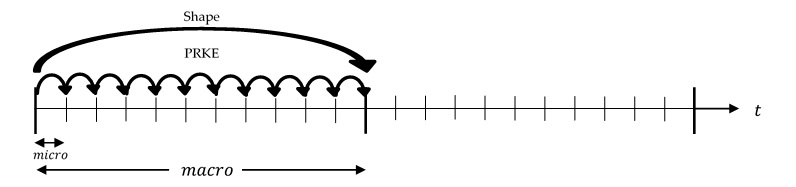
\includegraphics[width=\linewidth]{\FiguresDir/IQS_visualization.jpg}
\caption{IQS method visualization}
\label{fig:iqsviz}
\end{figure}

%%%%%%%%%%%%%%%%%%%%%%%%%%%%%%%%%%%%%%%%%%%%%%%%
\subsection{Operator Notation and Extension of IQS to Multigroup Transport Equations}
\label{sect:transport}

For simplicity, the previous section only described the IQS implementation using the neutron diffusion equation. However, deriving the IQS form for other neutron balance equations (e.g., transport, simplified transport, etc.) is very similar. To this end, we re-write the neutron conservation equations in operator form, shown in \eqt{eq:transport}. 
\be
\frac{1}{v^g}\frac{\partial \Psi^g}{\partial t} = \sum_{g'} \left(H^{g'\to g} + P_p^{g' \to g} \right) \Psi^{g'} - L^g\Psi^g + S_d^g
\label{eq:transport}
\ee
where $\Psi^g$ is the multigroup neutron flux (angular flux in the case of transport), $H^{g'\to g}$ is the scattering operator, $P_p^{g' \to g}$ is the prompt neutron production operator, $L^g$ is the loss operator, and $S_d^g$ is the delayed neutron source operator. Using \eqt{eq:flux}, the reader may easily obtain the functional form for these operators in the case of a diffusion approximation.
%
%Factorization is defined as $\Psi^g(\vec{r},\vec{\Omega},t)=p(t)\psi^g(\vec{r},\vec{\Omega},t)$ and the resulting shape equation is defined by \eqt{eq:tshape}.  
Next, the factorization $\Psi^g(\vec{r},\vec{\Omega},t)=p(t)\psi^g(\vec{r},\vec{\Omega},t)$ is introduced, where the shape is denoted by $\psi^g$, leading to the following shape equations, \eqt{eq:tshape}:
\be
\frac{1}{v^g}\frac{\partial \psi^g}{\partial t}  = \sum_{g'} \left(H^{g' \to g} + P_p^{g' \to g}\right) \psi^{g'} - \left( L^g + \frac{1}{v^g}\frac{1}{p}\frac{dp}{dt}\right) \psi^g + \frac{1}{p} S_d^g
\label{eq:tshape}
\ee
Finally, the PRKE parameters are defined by \eqts{eq:trmb}{eq:tb}, where 
$\left(\Psi^{*g},f^g\right) =$\\ $ \int_{4\pi}\int_D \Psi^{*g}(\vec{r},\vec{\Omega})f^g(\vec{r},\vec{\Omega})d^3r d^2\Omega$.
\be
\frac{\rho-\bar{\beta}}{\Lambda}=\frac{ \sum_{g=1}^G\left(\Psi^{*g},\sum_{g'}(H^{g' \to g}g+P_p^{g' \to g}-L^{g'}\delta_{g'g})\psi^{g'}\right)}{\sum_{g=1}^G\left(\Psi^{*g},\frac{1}{v^g}\psi^g\right)}
\label{eq:trmb}
\ee
\be
\frac{\bar{\beta}}{\Lambda}=\sum_{i=1}^I\frac{\bar{\beta}_i}{\Lambda}=\sum_{i=1}^I\frac{\sum_{g=1}^G(\Psi^{*g}, \sum_{g'} P_{d,i}^{g' \to g} \psi^{g'})}{\sum_{g=1}^G\left(\Psi^{*g},\frac{1}{v^g}\psi^g\right)}
\label{eq:tb}
\ee
where $P_{d,i}^{g' \to g}$ is the delayed-neutron operator for precursor group $i$. \\
\indent This section is simply meant to show the theoretical expandability of IQS to transport problems and its derivation in operator notation.  As stated previously, this research only applies and tests IQS with diffusion problems.

%%%%%%%%%%%%%%%%%%%%%%%%%%%%%%%%%%%%%%%%%%%%%%%%
\section{Iterative Solution Techniques}
\label{sect:iter}
%%%%%%%%%%%%%%%%%%%%%%%%%%%%%%%%%%%%%%%%%%%%%%%%

As we noted in \sct{sect:theory}, shape-PRKE equations are a nonlinear system and thus may be solved in a iterative manner.  Each macro time step can be iterated so the best shape is used to compute power at the micro time steps. Sissaoui et al. from \cite{Sissaoui_1995}, Koclas et al. from \cite{Koclas_1996}, Devooght et al. from \cite{Devooght_1984}, and Monier from \cite{Monier_diss} all use iterative techniques for their quasi-static simulations.  They all undergo a similar process:
\begin{itemize}
\item[\textit{Step 1:}] Compute the PRKE parameters at the end of the macro step using the last computed shape
\item[\textit{Step 2:}] Linearly interpolate the computed PRKE parameters over the macro step
\item[\textit{Step 3:}] Solve the PRKE on micro steps over the entire macro step
\item[\textit{Step 4:}] Solve the shape equation on the macro step using the computed values of $p$ and $dp/dt$.
\item[\textit{Step 5:}] Check if the shape solution has converged:
	\begin{itemize}
	\item \textit{No:} Repeat the same macro time step
	\item \textit{Yes:} Move on to the next macro time step
	\end{itemize}
\end{itemize}
This process can be visualized by \fig{fig:picard}.
\begin{figure}[!htpb]
\centering
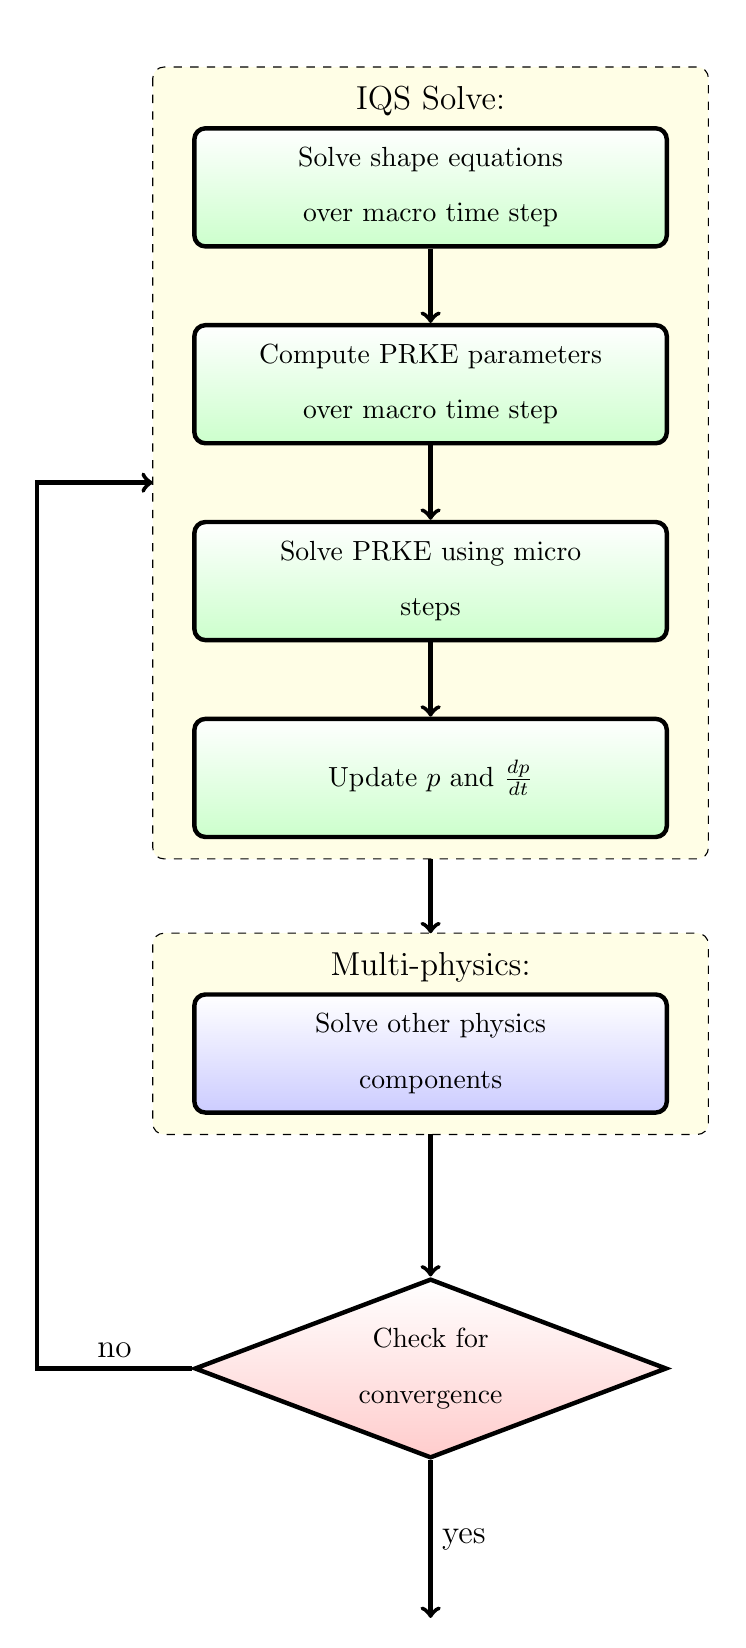
\begin{tikzpicture}[every node/.style = {font=\normalsize}]

\node[greenblock](p1) at (0,0) {Solve shape equations \\ over macro time step};
\node[greenblock](p2) at (0,-2.5) {Compute PRKE parameters \\ over macro time step};
\node[greenblock](p3) at (0,-5) {Solve PRKE using micro \\ steps};
\node[greenblock](p4) at (0,-7.5) {Update $p$ and $\frac{dp}{dt}$};
\node[blueblock2] (p5) at (0,-11) {Solve other physics \\ components};
\node[reddiamond] (check) at (0,-15) {Check for \\ convergence};
\node [above =0.1mm of p1] {\large{IQS Solve:}};
\node [above =0.1mm of p5] {\large{Multi-physics:}};

\tikzback{p1}{p1}{p4}{p4}{bk1}
\tikzback{p5}{p5}{p5}{p5}{bk2}

\draw[->,ultra thick](p1.south) -- (p2.north);
\draw[->,ultra thick](p2.south) -- (p3.north);
\draw[->,ultra thick](p3.south) -- (p4.north);
\draw [->,ultra thick] (p4.south)+(0,-0.25) -- node [above] {} (bk2-n);
\draw[->,ultra thick](p5.south)+(0,-0.25) -- (check.north);
%\draw[->,ultra thick](check.west) -- (-5,-15) -- node[above,sloped] {\large{no}}(-5,0) -- node[above] {}(bk1-w);
\draw[->,ultra thick](check.west) -- node[above,sloped] {\large{no}} (-5,-15) |-  node[above] {}(bk1-w);
\draw[->,ultra thick](check.south) -- node[right] {\large{yes}} ++(0,-2);

\end{tikzpicture}
\caption{Visualization of IQS fixed-point iteration process}
\label{fig:picard}
\end{figure}

The major difference between the methods of these authors is the convergence criteria used.  Sissaoui and Koclas \cite{Sissaoui_1995, Koclas_1996} use fixed point iteration where the criteria is the simply the normalized difference between the last two computed shapes.  Monier in \cite{Monier_diss} also does fixed point iterations with the same criteria, except the solution is scaled by $\frac{\sum_{g=1}^G\left(\phi^{*g},\frac{1}{v^g}\varphi^g(t_{n})\right)}{\sum_{g=1}^G\left(\phi^{*g},\frac{1}{v^g}\varphi^g(t_{n+1})\right)}$ after each iteration.  Devooght in \cite{Devooght_1984} does a Newton-SOR iteration where the residual of the shape function evaluation is the convergence criteria and next iteration's solution is computed using Newton-Raphson method.

These techniques are by no means an exhaustive list of the possible iteration techniques for IQS. Dulla et al. in \cite{Dulla2008} does an in depth analysis of the fixed point iteration technique most similar to Sissaoui and Koclas, involving convergence rates and solution results.  However, no comprehensive analysis of iteration techniques exists, comparing both Newton and fixed-point convergence rates.  The following sections describes each iteration technique investigated by this research.

%%%%%%%%%%%%%%%%%%%%%%%%%%%%%%%%%%%%%%%%%%%%%%%%
\subsection{Shape Convergence}

The most obvious convergence criteria is to observe the change in the shape from one iteration to the next.  Monier in \cite{Monier_diss} observes the $L^{\infty}$ norm of the shape for the convergence criteria, described in \eqt{eq:shape_Linf}.  However, any norm can be used for the criteria, so a $L^2$ norm is another possible criteria, described by \eqt{eq:shape_L2}.
\be
\frac{\text{max}\left|\varphi_{n}^{(k+1)} - \varphi_{n}^{(k)}\right|}{\text{max}\left|\varphi_{n}^{(k+1)}\right|} < \epsilon_{\varphi}
\label{eq:shape_Linf}
\ee 
\be
\frac{\norm{\varphi_{n}^{(k+1)} - \varphi_{n}^{(k)}}}{\norm{\varphi_{n}^{(k+1)}}} < \epsilon_{\varphi}
\label{eq:shape_L2}
\ee 

Where $n$ is the time step, $k$ is the iteration number, and $\epsilon_{\varphi}$ is the numerical criteria provided by a user. Through testing, iterations do not always converge; in this circumstance, the maximum number of iterations is reached.


%%%%%%%%%%%%%%%%%%%%%%%%%%%%%%%%%%%%%%%%%%%%%%%%
\subsection{Property Convergence}

Monier in \cite{Monier_diss} describes other properties, other than shape, to observe for convergence, shown in Equations \eqref{eq:rho_conv} - \eqref{eq:K_conv}.  These criteria can be added constraints to \eqt{eq:shape_Linf} or be in supplement to.
\be
\left(\frac{\rho}{\Lambda}\right)^{(k+1)} - \left(\frac{\rho}{\Lambda}\right)^{(k)} < \epsilon_{\rho}
\label{eq:rho_conv}
\ee
\be 
p_n^{k+1} - p_n^{k} < \epsilon_p
\label{eq:p_conv}
\ee
\be 
\frac{K_n^{(k+1)} - K_0}{K_0} < \epsilon_K
\label{eq:K_conv}
\ee

Where $K$ is the IQS uniqueness expression:
\be 
K_n^{(k+1)} = \sum_{g=1}^G\left(\phi^{*g},\frac{1}{v^g}\varphi_n^{g,(k+1)}\right)
\label{eq:K}
\ee

$\epsilon_{\rho}$ is the reactivity convergence criteria, $\epsilon_{p}$ is the amplitude convergence criteria, and $\epsilon_{K}$ is the constraint convergence criteria.

%%%%%%%%%%%%%%%%%%%%%%%%%%%%%%%%%%%%%%%%%%%%%%%%
\subsection{Solution Scaling}

In order to preserve the uniqueness criteria, it is beneficial to scale the shape such that the $K_n$ is constant, shown in \eqt{eq:shape_scale}.  This scaling can also be done after each iteration, to insure that the uniqueness criteria is satisfied whenever the shape is evaluated.
\be 
\varphi^{g}_n = \varphi^{g,(\text{last})}_n \frac{K_0}{K^{(\text{last})}_{n}}
\label{eq:shape_scale}
\ee

%%%%%%%%%%%%%%%%%%%%%%%%%%%%%%%%%%%%%%%%%%%%%%%%
\subsection{Preconditioned Jacobian-Free Newton-Krylov}
\label{sect:pjfnk}

By far, the most common nonlinear system iteration method in MOOSE is Preconditioned Jacobian-Free Newton-Krylov with Generalized Minimal RESidual method (GMRES) as the linear system solver.  This section only descirbes the methods' application to IQS; a very detailed description of PJFNK is transcribed by Knoll in \cite{PJFNK_Knoll}. Essentially, the IQS system of equations can be described by \eqt{eq:IQSsys}.  Where $A$ is a matrix operator, $\varphi$ is the solution vector, and $F$ is the forcing vector.
\be
A(\varphi(p))\varphi=F(\varphi,p,t)
\label{eq:IQSsys}
\ee
Applying the residual based Newton-method yields:
\be
J\delta\varphi = -R(\varphi,p)
\ee 
Where $J$ is the Jacobian matrix defined as $J_{ij}=\partial R_i/\partial\varphi_j$, $\delta\varphi$ is the error in the iterating solution, and $R$ is the residual vector defined as $A\varphi-F$ (most methods simply define the residual instead of evaluating this expression).  For IQS, a residual evaluation entails a PRKE parameter evaluation and the PRKE evaluation over the entire macro-step.  Applying a preconditioner $P$ yields:
\be 
(JP^{-1})(P\delta\varphi)=-R(\varphi,p)
\ee
This resulting system can be split into two systems, represented by \eqts{eq:PJFNK_1}{eq:PJFNK_2}.
\be 
(JP^{-1})w = -R(\varphi,p)
\label{eq:PJFNK_1}
\ee
\be 
\delta\varphi = P^{-1}w
\label{eq:PJFNK_2}
\ee
Solving \eqt{eq:PJFNK_1} requires the evaluation of Jacobian operator, which is done each GMRES iteration in two steps:
\begin{enumerate}
\item Approximately solve the preconditioner system for $y$: $Py=w$
\item Perform matrix-free Jacobian operation: $Jy\approx[R(\varphi+\epsilon y,p')-R(\varphi,p)]/\epsilon$
\end{enumerate}
This Jacobian operation is a finite difference approach.  $\epsilon$ is a perturbation scalar and $p'$ is the amplitude computed with PRKE parameters calculated from the perturbed shape.  For IQS, the PRKE and its parameters must be evaluated for the perturbed and original system, although the unperturbed residual is stored from the beginning of the PJFNK iteration.

%%%%%%%%%%%%%%%%%%%%%%%%%%%%%%%%%%%%%%%%%%%%%%%%
\section{Predictor-Corrector version of IQS (IQS P-C)}
\label{sect:pc}
%%%%%%%%%%%%%%%%%%%%%%%%%%%%%%%%%%%%%%%%%%%%%%%%

The Predictor-Corrector (P-C) version of IQS factorizes the flux and derives the PRKE the same way as the standard version, but the solution of the coupled system of equations is different.  In the IQS P-C version, the flux equations (not the shape equations) are solved (represented by \eqts{eq:flux}{eq:precursor}) in order to obtain a predicted flux solution. This predicted flux is then converted to a shape by rescaling it as follows:
\be
\varphi^g_{n+1} = \underbrace{\phi^g_{n+1}}_{\text{predicted}} \frac{K_0}{K_{n+1}}
\label{eq:rescale}
\ee
where the scaling factors are given by
\be
K_{n+1} =\sum_{g=1}^G\left(\phi^{*g},\frac{1}{v^g}\phi^g_{n+1}\right)
\ee
\be
K_{0} =\sum_{g=1}^G\left(\phi^{*g},\frac{1}{v^g}\varphi^g_{n+1}\right)=\sum_{g=1}^G\left(\phi^{*g},\frac{1}{v^g}\phi^g_{0}\right)
\ee

The PRKE parameters are then computed with this shape using \eqtss{eq:rmb}{eq:l} and interpolated over the macro step, then the PRKE ODE system is solved on the micro time scale.  With the newly computed amplitude, the shape is rescaled into a flux and the final corrected flux is given by:
\be
\underbrace{\phi^g_{n+1}}_{\text{corrected}} = p_{n+1} \times \varphi^g_{n+1} \,.
\ee

The advantage to the predictor-corrector method is there is no iteration necessary for this method and, in turn, is much simpler and faster than the standard IQS.  Ikeda et al. in \cite{Ikeda_2001} and Goluoglu et al. in \cite{Goluoglu_2001} both use IQS P-C for complex, three-dimensional problems.  Their results prove IQS P-C to be impressively effective, despite the de-coupling of the system.  Dulla et al. in \cite{Dulla2008} also describes an in depth comparison of IQS P-C with traditional IQS.


%%%%%%%%%%%%%%%%%%%%%%%%%%%%%%%%%%%%%%%%%%%%%%%%
\section{Temperature Feedback}
\label{sect:mp}
%%%%%%%%%%%%%%%%%%%%%%%%%%%%%%%%%%%%%%%%%%%%%%%%

IQS is first and foremost a nuclear reactor simulation method.  In nuclear reactors, multiple physics affect the profile of the neutron flux.  One of the simplest examples of mulitphysics reactor simulations is adiabatic heat up with Doppler feedback. The principle of Doppler feedback is that fission in a fuel causes the material to increase temperature and induces a change in the neutronics properties.  The material heat up is described by \eqt{eq:temp}; where $\rho$ is the material density, $c_p$ is the specific heat, $T$ is temperature, and $\kappa_f$ is the energy released per fission \cite{ANL_BPB}. The change in temperature of the material mainly affects the thermal macroscopic absorption cross section described by \eqt{eq:dopp} \cite{ANL_BPB}.

\be
\rho c_p \frac{\partial T(\vec{r},t)}{\partial t} = \kappa_f \sum^G_{g=1}\Sigma_f^g \phi^g(\vec{r},t)
\label{eq:temp}
\ee

\be
\Sigma_a^{thermal}(\vec{r},t) = \Sigma_a^{thermal}(\vec{r},0)\left[1+\gamma\left(\sqrt{T}-\sqrt{T_0}\right)\right]
\label{eq:dopp}
\ee

%%%%%%%%%%%%%%%%%%%%%%%%%%%%%%%%%%%%%%%%%%%%%%%%
\subsection{Temperature Evaluation}

Temperature evaluation (\eqt{eq:temp}) is quite similar to the evaluation of the delayed neutron precursors from \sct{sect:dnp}. A typical implicit solver would simply use the interpolated flux at end of the temperature time step for the right hand side of the equation, a theta-method discretization.  However, IQS has much more information about the profile of the flux along the time step because of the micro-step amplitude evaluation.  Therefore, it is possible to solve for temperature using a semi-analytical approach, shown by \eqt{eq:temp_an}.
\be
T^{n+1} = T^n + \frac{\kappa_f}{\rho c_p} \left(a_2 \varphi^{n+1} + a_1 \varphi^{n}\right)
\label{eq:temp_an}
\ee
Where $n$ corresponds to the beginning of the temperature step.  $a_1$ and $a_2$ are integration coefficients defined by \eqt{eq:a1} and \eqt{eq:a2}.  Any interpolation of the amplitude along the micro steps is possible for the integration, this application uses piece-wise linear.
\be
a_1 = \int_{t_n}^{t_{n+1}}\left(\frac{t_{n+1}-t'}{\Delta t}\right)p(t')dt'
\label{eq:a1}
\ee
\be
a_2 = \int_{t_n}^{t_{n+1}}\left(\frac{t'-t_n}{\Delta t}\right)p(t')dt'
\label{eq:a2}
\ee

%%%%%%%%%%%%%%%%%%%%%%%%%%%%%%%%%%%%%%%%%%%%%%%%
\subsection{Intermediate Time Scale}

For IQS, this temperature feedback affects both the shape equation and the reactivity of the PRKE; thus, it is an additional nonlinear component to the already coupled shape-amplitude equations. In foresight to the application of this component, temperature is much more time dependent than the shape, but less so than the amplitude.  Therefore, the evaluation of temperature will have its own time scale.  A possible solution process for a problem with temperature feedback will have time three time scales portrayed in \fig{fig:time}.  The first time scale is the shape solve, the second is the temperature evaluation as well as the computation of PRKE parameters, and the third is the PRKE scale.  It is important to note that the number of time steps in each scale is arbitrary and meant only for visual purposes.

\begin{figure}[htpb!]
\centering
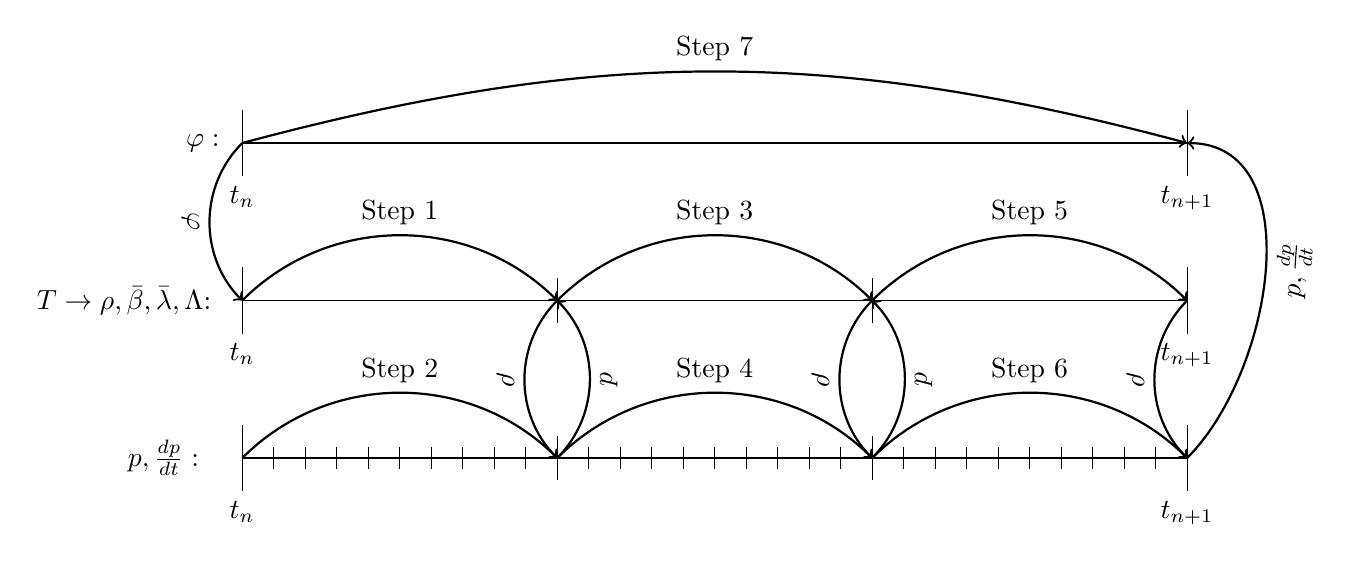
\begin{tikzpicture}[scale=2]
%Shape
\draw[] (0,2) -- (6,2) ;
\foreach \x in  {0,6}
\draw[shift={(\x,2)},color=black] (0pt,6pt) -- (0pt,-6pt);
\draw[shift={(0,2)},color=black] (0pt,0pt) -- (0pt,-6pt) node[below] {$t_n$};
\draw[shift={(6,2)},color=black] (0pt,0pt) -- (0pt,-6pt) node[below] {$t_{n+1}$};
\node(shape) at (-.25,2) {$\varphi:$};

%Temp/Params
\draw[] (0,1) -- (6,1) ;
\foreach \x in  {0,6}
\draw[shift={(\x,1)},color=black] (0pt,6pt) -- (0pt,-6pt);
\foreach \x in  {2,4}
\draw[shift={(\x,1)},color=black] (0pt,4pt) -- (0pt,-4pt);
\draw[shift={(0,1)},color=black] (0pt,0pt) -- (0pt,-6pt) node[below] {$t_n$};
\draw[shift={(6,1)},color=black] (0pt,0pt) -- (0pt,-6pt) node[below] {$t_{n+1}$};
\node(temp) at (-.75,1) {$T \rightarrow \rho, \bar{\beta}, \bar{\lambda}, \Lambda$:};

% PRKE
\draw[] (0,0) -- (6,0) ;
\foreach \x in  {0,6}
\draw[shift={(\x,0)},color=black] (0pt,6pt) -- (0pt,-6pt);
\foreach \x in  {0,2,4,6}
\draw[shift={(\x,0)},color=black] (0pt,4pt) -- (0pt,-4pt);
\foreach \x in  {0,0.2,0.4,0.6,0.8,1,1.2,1.4,1.6,1.8,2,2.2,2.4,2.6,2.8,3,3.2,3.4,3.6,3.8,4,4.2,4.4,4.6,4.8,5,5.2,5.4,5.6,5.8,6}
\draw[shift={(\x,0)},color=black] (0pt,2pt) -- (0pt,-2pt);
\draw[shift={(0,0)},color=black] (0pt,0pt) -- (0pt,-6pt) node[below] {$t_n$};
\draw[shift={(6,0)},color=black] (0pt,0pt) -- (0pt,-6pt) node[below] {$t_{n+1}$};
\node(prke) at (-.5,0) {$p, \frac{dp}{dt}:$};

\draw (0,0) edge[out=45,in=135,->,thick] node[above,sloped] {Step 2} (2,0);
\draw (2,0) edge[out=45,in=135,->,thick] node[above,sloped] {Step 4} (4,0);
\draw (4,0) edge[out=45,in=135,->,thick] node[above,sloped] {Step 6} (6,0);
\draw (0,1) edge[out=45,in=135,->,thick] node[above,sloped] {Step 1} (2,1);
\draw (2,1) edge[out=45,in=135,->,thick] node[above,sloped] {Step 3} (4,1);
\draw (4,1) edge[out=45,in=135,->,thick] node[above,sloped] {Step 5} (6,1);
\draw (0,2) edge[out=15,in=165,->,thick] node[above,sloped] {Step 7} (6,2);

\draw (0,2) edge[out=-135,in=135,->,thick] node[below,sloped] {$\varphi$} (0,1);
\draw (2,1) edge[out=-135,in=135,->,thick] node[below,sloped] {$\rho$} (2,0);
\draw (2,0) edge[out=45,in=-45,->,thick] node[below,sloped] {$p$} (2,1);
\draw (4,1) edge[out=-135,in=135,->,thick] node[below,sloped] {$\rho$} (4,0);
\draw (4,0) edge[out=45,in=-45,->,thick] node[below,sloped] {$p$} (4,1);
\draw (6,1) edge[out=-135,in=135,->,thick] node[below,sloped] {$\rho$} (6,0);
\draw (6,0) edge[out=45,in=0,->,thick] node[below,sloped] {$p, \frac{dp}{dt}$} (6,2);

\end{tikzpicture}
\caption{Time scales and process of IQS with temperature feedback}
\label{fig:time}
\end{figure}


%%%%%%%%%%%%%%%%%%%%%%%%%%%%%%%%%%%%%%%%%%%%%%%%
\subsection{Dynamical Time Scale Analysis}
\label{sect:tau}

The temporal variance of flux, shape, temperature, and amplitude can be quantified by defining a dynamical time scale ($\tau$) for each physics.  A small value $\tau$ means the variable is quickly varying in time and consequently needs relatively small time steps for accuracy, vice-versa for large $\tau$.  The general definition of $\tau$ is defined by \eqt{eq:tau1}, where $\theta$ is the physic component of interest.  
\be
\tau = \frac{1}{\left|\frac{1}{\theta}\frac{d\theta}{dt}\right|}
\label{eq:tau1}
\ee
Since each variable in discretized in time, a finite difference approximation will be made for the $\frac{d\theta}{dt}$ term and the average between the two corresponding time steps will be made for the $\frac{1}{\theta}$ term.  Additionally, $\tau$ is spatially dependent for flux and temperature, but only the time dependent behavior of this quantity is of interest.  Therefore, the $L^2$ norm of each term will be used to compute the approximate time scale ($\tilde{\tau}$), formally defined by \eqt{eq:tau2}.  $\theta$ represents a summation over groups for flux and shape.
\be
\tilde{\tau}_{n+1} = \frac{\norm{\theta_{n+1} + \theta_{n}}}{2}\frac{\Delta t}{\norm{\theta_{n+1} - \theta_{n}}}
\label{eq:tau2}
\ee
%
According to the a priori hypothesis from previous sections, $\tau$ is large for shape, somewhat smaller for temperature, and much smaller for amplitude and flux.


%%%%%%%%%%%%%%%%%%%%%%%%%%%%%%%%%%%%%%%%%%%%%%%%
\subsection{Programming Logic}

The couplings between temperature, amplitude, and shape are all nonlinear, so iteration processes are needed for each time scale.  The amplitude and temperature need to be iterated on the middle time scale until convergence on each temperature step.  Then another iterative process needs to occur in the shape time scale on all three variables. \fig{fig:proc} shows the programming diagram implement to execute this process. The time increment of $\Delta t/3$ for the temperature solve is arbitrary and is meant only to match \fig{fig:time} where three temperature updates have been used as illustration.


\begin{figure}[!htpb]
\centering
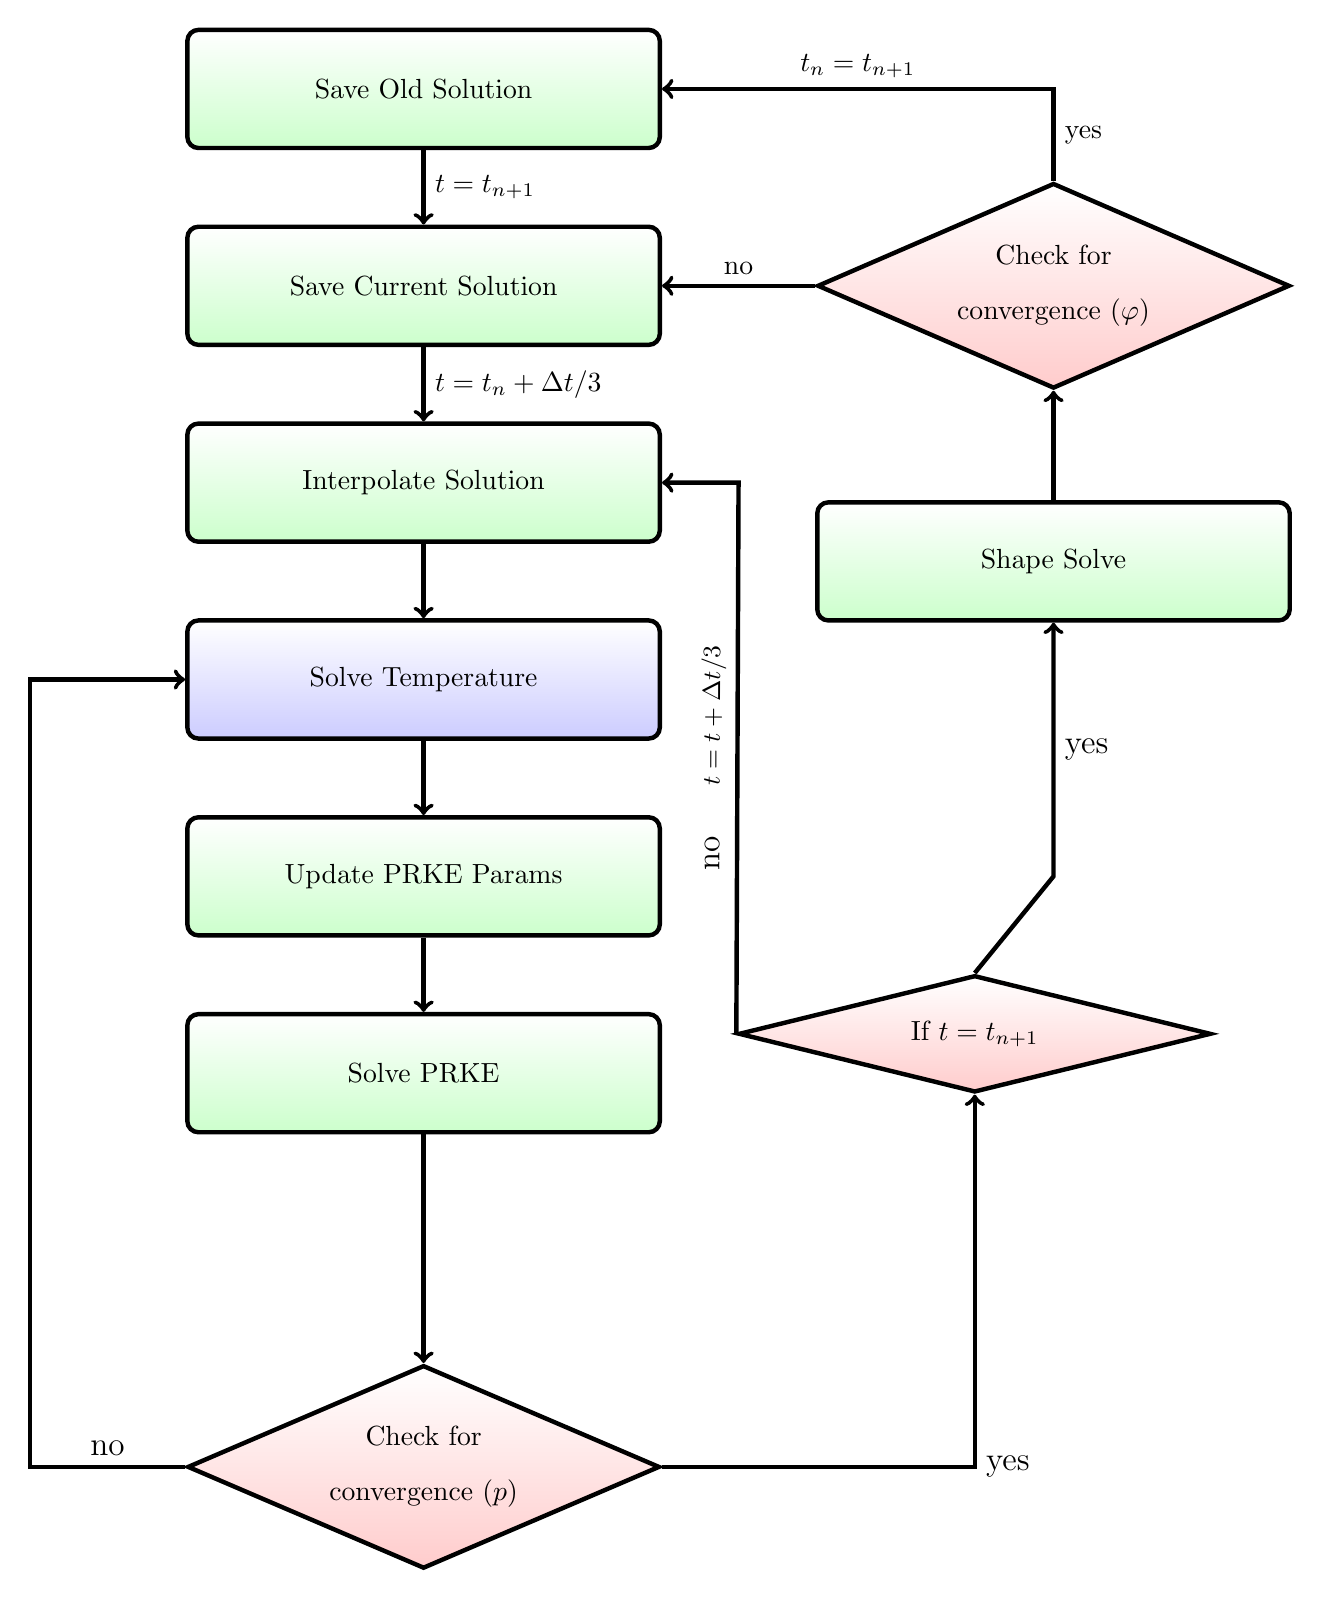
\begin{tikzpicture}[every node/.style = {font=\normalsize}]

\node[greenblock](p1) at (0,0) {Save Old Solution};
\node[greenblock](p2) at (0,-2.5) {Save Current Solution};
\node[greenblock](p3) at (0,-5) {Interpolate Solution};
\node[blueblock2](p4) at (0,-7.5) {Solve Temperature};
\node[greenblock] (p5) at (0,-10) {Update PRKE Params};
\node[greenblock] (p6) at (0,-12.5) {Solve PRKE};
\node[reddiamond] (check1) at (0,-17.5) {Check for \\ convergence ($p$)};
\node[reddiamond] (check2) at (7,-12) {If $t=t_{n+1}$};
\node[greenblock] (p7) at (8,-6) {Shape Solve};
\node[reddiamond] (check3) at (8,-2.5) {Check for \\ convergence ($\varphi$)};
%\node [above =0.1mm of p1] {\large{IQS Solve:}};
%\node [above =0.1mm of p5] {\large{Multi-physics:}};

%\tikzback{p1}{p1}{p4}{p4}{bk1}
%\tikzback{p5}{p5}{p5}{p5}{bk2}

\draw[->,ultra thick](p1.south) -- node[right] {$t=t_{n+1}$}(p2.north);
\draw[->,ultra thick](p2.south) -- node[right] {$t=t_{n}+\Delta t/3$}(p3.north);
\draw[->,ultra thick](p3.south) -- (p4.north);
\draw [->,ultra thick] (p4.south)-- (p5.north);
\draw[->,ultra thick](p5.south) -- (p6.north);
\draw[->,ultra thick](p6.south) -- (check1.north);
\draw[->,ultra thick](check1.west) -- node[above,sloped] {\large{no}} (-5,-17.5) |-  (p4.west);
\draw[->,ultra thick](check1.east) -| node[right] {\large{yes}} (check2.south);
\draw[->,ultra thick](check2.west) -- node[above,sloped] {\large{no}\small \qq $t=t+\Delta t/3$} (4,-5) -- (p3.east);
\draw[->,ultra thick](check2.north) --  (8,-10) -- node[right] {\large{yes}} (p7.south);
\draw[->,ultra thick](p7.north) -- (check3.south);
\draw[->,ultra thick](check3.west) -- node[above] {no} (p2.east);
\draw[->,ultra thick](check3.north) -- node[right] {yes} (8,0) -- node[above] {$t_n=t_{n+1}$} (p1.east);

\end{tikzpicture}
\caption{Visualization of fixed-point iteration and temperature update process for IQS}
\label{fig:proc}
\end{figure}


%%%%%%%%%%%%%%%%%%%%%%%%%%%%%%%%%%%%%%%%%%%%%%%%
\section{Time Discretization Schemes}
\label{sect:dt}
%%%%%%%%%%%%%%%%%%%%%%%%%%%%%%%%%%%%%%%%%%%%%%%%

A vital part of the verification and validation for IQS is analyzing error convergence.  Since any time discretization scheme is capable of being applied to the shape equation of IQS, it is important to investigate IQS's performance to a variety of these schemes.  There is lack of literature that applies IQS to schemes other than implicit Euler; higher order schemes are never rigorously tested.  This research intends to apply a variety of schemes, including implicit Euler, Crank-Nicholson, backward difference formula (BDF), and diagonally implicit Runge-Kutta (DIRK), to test stability and error convergence.  For brevity in the following sections, the shape-diffusion equation is represented by a general operator notation, described by \eqt{eq:shape_mat}.
\be 
IV\frac{\partial \varphi}{\partial t} = A\varphi+b
\label{eq:shape_mat}
\ee
Where $IV$ is the inverse velocity operator, $A$ contains all the operations on $\varphi$ from the left-hand-side of \eqt{eq:shape}, and $b$ is the source from the precursors. 

%%%%%%%%%%%%%%%%%%%%%%%%%%%%%%%%%%%%%%%%%%%%%%%%
\subsection{Theta Method Time Discretization}
\label{sect:theta}

A fairly simple way to evaluate the shape equation is to employ the $\theta$-scheme ($0\le\theta\le1$, explicit when $\theta=0$, implicit when $\theta=1$, and Crank-Nicholson when $\theta=1/2$) \cite{Ferziger}.  Generally, if there is a function $u$ whose governing equation is $\frac{du}{dt}=f(u,t)$, then the $\theta$-discretization is:
\be
\frac{u^{n+1}-u^n}{\Delta t}=(1-\theta)f(u^n,t) + \theta f(u^{n+1},t) \,.
\ee
Where $n$ is the previous time step and $n+1$ is the time step being evaluated. Applying this to \eqt{eq:shape_mat} yields:
\be
\varphi_{n+1} = (IV-\Delta t A_{n+1})^{-1}\left[\Delta t(1-\theta)(A_n\varphi_n+b_n) + \Delta t\theta b_{n+1} + IV\varphi_n\right]
\ee

%%%%%%%%%%%%%%%%%%%%%%%%%%%%%%%%%%%%%%%%%%%%%%%%
\subsection{Backward Difference Formulae}

An extension of implicit discretization is the backward difference formulae (BDF) \cite{Gear:2007}.  BDF's can increase the order of error convergence by interpolating solutions from previous time steps. The general formula for BDF is described by \eqt{eq:bdf}.
\be 
\varphi_{n+1} = (IV-\Delta t A_{n+1})^{-1}\left[IV\sum_{j=1}^{k}\alpha_{j}^{k}\varphi_{n-(k-j)} +
\Delta t \alpha_{k+1}^{k} b_{n+1}\right]
\label{eq:bdf}
\ee
where $k$ is the order of the error convergence and $\alpha_{j}^{k}$ (vector of length $k+1$) are coefficients chosen such that the temporal truncation error is minimized.  \tbl{tab:bdfa} shows the values of $\alpha$ for every order implemented in this thesis. The benefit of using BDF is that any order of convergence can be applied and are unconditionally stable up through fourth order, so the IQS approximation can easily be validated for high order discretization.

\begin{table}
\centering
\begin{tabular}{c|lllll}
\hline
Order ($k$) & $\alpha_{1}^{k}$ & $\alpha_{2}^{k}$ & $\alpha_{3}^{k}$ & $\alpha_{4}^{k}$ & $\alpha_{5}^{k}$ \\
\hline
1 & 1 & 1 & & & \\
2 & -1/3 & 4/3 & 2/3 & & \\
3 & 2/11 & -9/11 & 18/11 & 6/11 & \\
4 & -3/25 & 16/25 & -36/25 & 48/25 & 12/25 \\
\hline
\end{tabular}
\caption{$\alpha$ values for relevant BDF methods}
\label{tab:bdfa}
\end{table}

%%%%%%%%%%%%%%%%%%%%%%%%%%%%%%%%%%%%%%%%%%%%%%%%
\subsection{Singly-Diagonally-Implicit Runge-Kutta Method}

Singly-Diagonally-Implicit Runge-Kutta Method (SDIRK) is a powerful discretization method that involves solving the linear system in stages to reach a high order solution \cite{SDIRK}.  Generally, the method can be depicted by using a system where $dy/dt=f(t,y)$ and \eqt{eq:sdirk}.
\be 
y_{n+1} = y_n + \Delta t\sum_{i=1}^s b_ik_i
\label{eq:sdirk}
\ee
Where,
\be 
k_i = f(t_n+c_i\Delta t, y_n+\Delta t \sum_{j=1}^{i} a_{ij}k_j)
\ee
The coefficients $a_{ij}$, $b_i$, and $c_i$ can be represented by a Butcher tableau:
\begin{center}
\begin{tabular}{c|cccc}
$c_1$ & $a_{11}$ & &  & \\
'$c_2$ & $a_{21}$ & $a_{22}$ & & \\
$\vdots$ & $\vdots$ & $\vdots$ & $\ddots$ & \\
$c_s$ & $a_{s1}$ & $a_{s2}$ & $\ldots$ & $a_{ss}$\\
\hline
&$b_1$ & $b_2$ & $\ldots$ & $b_s$
\end{tabular}
\end{center}
An example used extensively in this research is SDIRK33, which is a third-order method with three stages.
\begin{center}
\begin{tabular}{c|ccc}
$\lambda$ & $\lambda$ & & \\
$\frac{1}{2}(1+\lambda)$ & $\frac{1}{2}(1-\lambda)$ & $\lambda$ & \\
$1$ & $\frac{1}{4}(-1+16\lambda-6\lambda^2)$ & $\frac{1}{4}(5-20\lambda+6\lambda^2)$ & $\lambda$\\
\hline
 & $\frac{1}{4}(-1+16\lambda-6\lambda^2)$ & $\frac{1}{4}(5-20\lambda+6\lambda^2)$ & $\lambda$
\end{tabular}
\end{center}
Where $\lambda\approx0.4358665215$ satisfies $1-9\lambda+18\lambda^2-6\lambda^3=0$.

%%%%%%%%%%%%%%%%%%%%%%%%%%%%%%%%%%%%%%%%%%%%%%%%
\subsection{Time Adaptation}

IQS aims at reducing the time discretization error in the flux solution by splitting the flux into an amplitude (highly resolved at a micro time scale) and a shape (whose time-dependence is weaker than that of the flux itself). Thus, by construction, the IQS approach may employ larger time-step sizes for comparable temporal error. Further enhancements can be gained by using time adaptation (or time step control) in order to increase or reduce the macro time step size for the shape evaluation, depending on error estimates. A step-doubling technique is chosen as the time adaptation technique \cite{NumC}. The step doubling technique involves estimating the local error for a certain time step by taking the difference between a solution with one full step ($\varphi^g_{\Delta t}$) and a solution with two half steps ($\varphi^g_{\Delta t/2}$). Note: $\varphi$ is changed to $\phi$ for implicit discretization and IQS P-C.

The relative error is computed as follows:
\be
e_n = \frac{\norm{\sum_{g=1}^G\varphi^g_{\Delta t/2} - \sum_{g=1}^G\varphi^g_{\Delta t}}}{\text{max}\left(\norm{\sum_{g=1}^G\varphi^g_{\Delta t/2}},\norm{\sum_{g=1}^G\varphi^g_{\Delta t}}\right)}
\label{eq:edt2}
\ee
If the error is smaller than the user-specified tolerance, $e_{tol}$, the time step is accepted. In addition, a new time step size is estimated as follows:
\be
\Delta t_{new} = S \Delta t \left(\frac{e_{tol}}{e_n}\right)^{\frac{1}{1+q}}
\label{eq:dt2}
\ee
Where $q$ is the convergence order of the time integration scheme being used and $S\simeq 0.8$ is a safety factor. If the error is larger than the user-specified tolerance, the time step is rejected. A new time step size is estimated using  \eqt{eq:edt2} as well. This process can be visualized by \figs{fig:dt2_1}{fig:dt2_2}.  Where a step involves a full convergence of shape, amplitude, and any multiphysics on the respective time step.

To investigate IQS's performance with step-doubling time adaptation, the adaptation will be applied to implicit discretization method, traditional IQS, and IQS P-C.  Each of these methods will be applied to several diffusion problems; the number of time steps taken and the resulting error will be used to compare the methods.

\begin{figure}[htpb!]
\centering
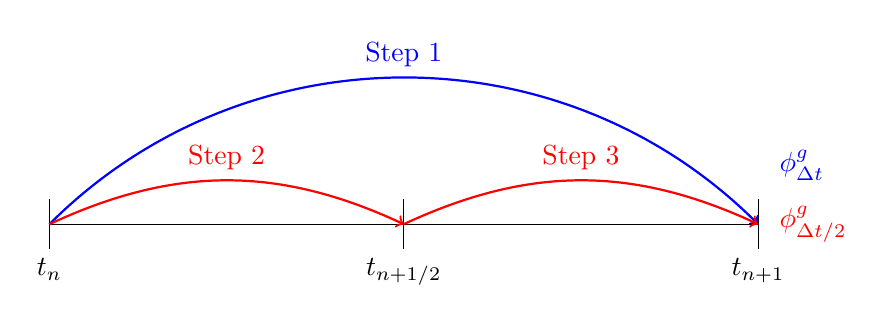
\begin{tikzpicture}[scale=1.5]
\draw[] (0,2) -- (6,2) ;
\foreach \x in  {0,3,6}
\draw[shift={(\x,2)},color=black] (0pt,6pt) -- (0pt,-6pt);
\draw[shift={(0,2)},color=black] (0pt,0pt) -- (0pt,-6pt) node[below] {$t_n$};
\draw[shift={(3,2)},color=black] (0pt,0pt) -- (0pt,-6pt) node[below] {$t_{n+1/2}$};
\draw[shift={(6,2)},color=black] (0pt,0pt) -- (0pt,-6pt) node[below] {$t_{n+1}$};
\draw (0,2) edge[out=45,in=135,->,thick,blue] node[above,sloped] {\tcb{Step 1}} (6,2);
\draw (0,2) edge[out=25,in=155,->,thick,red] node[above,sloped] {\tcr{Step 2}} (3,2);
\draw (3,2) edge[out=25,in=155,->,thick,red] node[above,sloped] {\tcr{Step 3}} (6,2);
\node[anchor=west](shape) at (6.1,2.5) {$\tcb{\phi_{\Delta t}^g}$};
\node[anchor=west](shape) at (6.1,2) {$\tcr{\phi_{\Delta t/2}^g}$};

\end{tikzpicture}
\caption{Visualization of step doubling process on time-line}
\label{fig:dt2_1}
\end{figure}

\begin{figure}[!htpb]
\centering
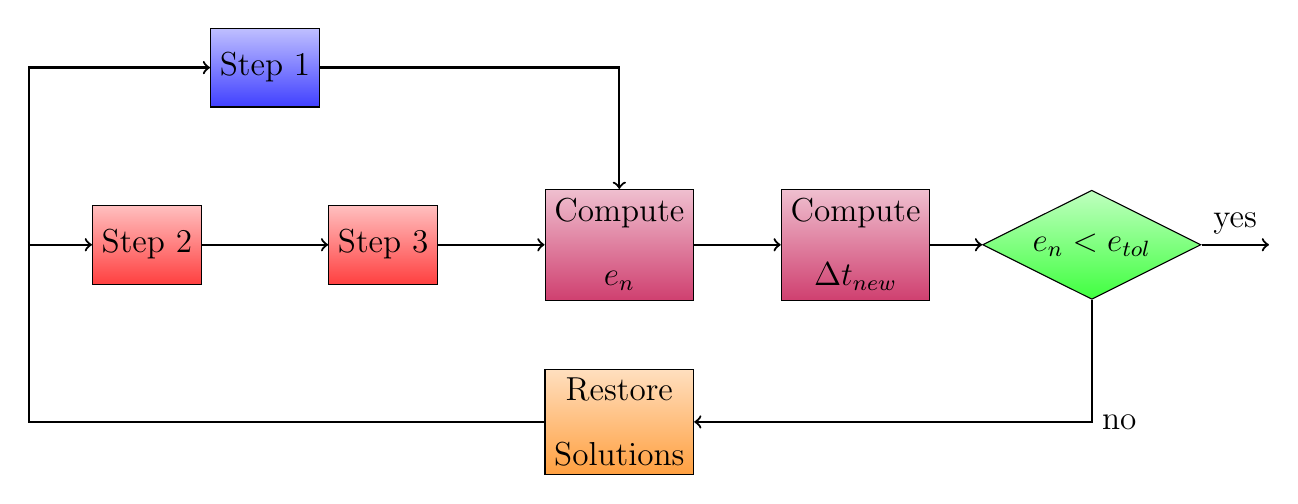
\begin{tikzpicture}[every node/.style = {font=\large},scale=0.75]

\node[blueblock](p1) at (-6,3) {Step 1} ;
\node[redblock](p2) at (-8,0) {Step 2} ;
\node[redblock](p3) at (-4,0) {Step 3} ;
\node[purpleblock](p4) at (0,0) {Compute \\ $e_n$};
\node[purpleblock](p5) at (4,0) {Compute  \\ $\Delta t_{new}$};
\node[greendiamond](p6) at (8,0) {$e_n < e_{tol}$};
\node[orangeblock](p7) at (0,-3) {Restore \\ Solutions};

\draw[->,thick](p1.east) -| (p4.north);
\draw[->,thick](p2.east) -- (p3.west);
\draw[->,thick](p3.east) -- (p4.west);
\draw[->,thick](p4.east) -- (p5.west);
\draw[->,thick](p5.east) -- (p6.west);
\draw[->,thick](p6.south) |- node[right] {no} (p7.east);
\draw[->,thick](p6.east) -- node[above] {yes} (11,0);
\draw[->,thick](p7.west) -| (-10,0) -- (p2.west);
\draw[->,thick](p7.west) -| (-10,0) |- (p1.west);

\end{tikzpicture}
\caption{Visualization of step doubling process with coding logic}
\label{fig:dt2_2}
\end{figure}

%%%%%%%%%%%%%%%%%%%%%%%%%%%%%%%%%%%%%%%%%%%%%%%%
\section{Delayed Neutron Precursor Updates}
\label{sect:dnp}
%%%%%%%%%%%%%%%%%%%%%%%%%%%%%%%%%%%%%%%%%%%%%%%%

This section presents the time-integration method used to solve coupled flux/shape and precursor equations, represented by Equations~\eqref{eq:flux}/\eqref{eq:shape}~and~\eqref{eq:precursor}/\eqref{eq:prec}. First, we note that we could keep this system of two time-dependent equations and solve it as a coupled system. However, this is unnecessary and a memory expensive endeavor because the precursor equation is only an ODE and not a PDE. Instead, one may discretize in time the shape equation, which typically requires the knowledge of the precursor concentrations at the end of the time step. This precursor value is taken from the solution, numerical or analytical, of the precursors ODE.

%%%%%%%%%%%%%%%%%%%%%%%%%%%%%%%%%%%%%%%%%%%%%%%%
\subsection{Precursor Evaluation Using Theta Method Time Discretization}

A common precursor evaluation technique is using the theta method, described in \sct{sect:theta}. Applying this to \eqt{eq:prec}:
\be
\frac{C^{n+1}-C^n}{\Delta t}=(1-\theta)\beta S_f^np^n-(1-\theta)\lambda C^n + \theta\beta S_f^{n+1}p^{n+1}-\theta\lambda C^{n+1}
\ee
Where $S_f$ is the fission source equivalent for shape ($S_f^n=(\nu\Sigma_f)^n\varphi^n$). Rearranging to solve for the precursor at the end of the time step yields
\be
C^{n+1} = \frac{1-(1-\theta)\Delta t\lambda}{1+\theta\Delta t\lambda}C^n + \frac{(1-\theta)\Delta t \beta}{1+\theta\Delta t\lambda}S_f^n p^n +  \frac{\theta\Delta t \beta}{1+\theta\Delta t\lambda}S_f^{n+1} p^{n+1}
\label{eq:dnp_theta}
\ee
Reporting this value of $C^{n+1}$, one can solve for the shape $\varphi^{n+1}$ as a function of $\varphi^n$ and $C^n$ (and $p^n$, $p^{n+1}$, $dp/dt|_n$ and  $dp/dt|_{n+1}$).
Once $\varphi^{n+1}$ has been determined, $C^{n+1}$ is updated.  Applying this technique to implicit discretization is done by changing the definition the fission source ($S_f^n=(\nu\Sigma_f)^n\phi^n$) and eliminating all $p$ terms.

%%%%%%%%%%%%%%%%%%%%%%%%%%%%%%%%%%%%%%%%%%%%%%%%
\subsection{Analytical Precursor Integration}

Another technique to evaluating the precursor equation is to use a exponential operator and integrate the time derivative analytically.  Applying this operation to \eqt{eq:prec} yields:
\be
C^{n+1} =  C^n e^{-\lambda (t_{n+1} - t_n) }  + \int_{t_n}^{t_{n+1}} \beta(t') S_f(t') p(t')e^{-\lambda (t_{n+1}-t')}dt'
\label{eq:prec_an}
\ee
Again, this can be applied to implicit discretization by altering the definition of the fission source and eliminating $p$.  Because $S_f$ is not known continuously over the time step, the integration can be done using any schemet (Riemann, trapezoid, Simpson's, etc.). However, there is a very accurate representation of $p(t)$ over the macro step from the PRKE solve. In order to utilize this information, another possibility is to interpolate $S_f$ linearly over the macro step.  Such that:
\be
S_f(t) = \frac{t_{n+1}-t}{t_{n+1}-t_n}S_f^n  + \frac{t-t_n}{t_{n+1}-t_n}S_f^{n+1}  \quad t_n \le t \le t_{n+1}
\ee
Applying this to \eqt{eq:prec_an} yields:
\be
C^{n+1} = C^n e^{-\lambda \Delta t} + \left(\hat{a}_2 S_f^{n+1}+\hat{a}_1 S_f^n\right)\beta
\label{eq:dnp_an}
\ee
With integration coefficients defined as:
\begin{align}
&\hat{a}_1= \int_{t_n}^{t_{n+1}}\frac{t_{n+1}-t'}{\Delta t}p(t')e^{-\lambda(t_{n+1}-t')}dt' \\
&\hat{a}_2 = \int_{t_n}^{t_{n+1}}\frac{t'-t_n}{\Delta t}p(t')e^{-\lambda(t_{n+1}-t')}dt'
\end{align}
The amplitude $(p)$ is included in the integration coefficient because it has been highly accurately calculated in the micro step scheme, so a piecewise interpolation (linear, cubic, etc.) between those points can be done to maximize accuracy.



%%%%%%%%%%%%%%%%%%%%%%%%%%%%%%%%%%%%%%%%%%%%%%%%
%%%%%%%%%%%%%%%%%%%%%%%%%%%%%%%%%%%%%%%%%%%%%%%%
\section{Rattlesnake Implementation}
%%%%%%%%%%%%%%%%%%%%%%%%%%%%%%%%%%%%%%%%%%%%%%%%
%%%%%%%%%%%%%%%%%%%%%%%%%%%%%%%%%%%%%%%%%%%%%%%%

Rattlesnake is a MOOSE-based application developed INL specific to solving radiation transport problems with multiphysics capabilities.  MOOSE is a finite-element based, multiphysics framework that gives the general architecture for the development of physics application like Rattlesnake.   At the heart of Rattlesnake is the action system, which provides a means to consolidate the MOOSE input syntax (which can be quite larger for multigroup transport simulations), so that a user does not have to define every kernel, variable, etc., used in the problem. Rather, the user inputs an equation description 
(e.g., Diffusion, S$_n$, P$_n$, etc.) and a solution method (e.g., SAAF, LS, CFEM, DFEM, etc.), and the action system will incorporate all the necessary physics involved (kernels, boundary conditions, postprocessor, etc.).

 
%%%%%%%%%%%%%%%%%%%%%%%%%%%%%%%%%%%%%%%%%%%%%%%%
\subsection{Executioner}
%%%%%%%%%%%%%%%%%%%%%%%%%%%%%%%%%%%%%%%%%%%%%%%%

An IQS excecutioner was created to implement the IQS method. The IQS executioner derives from the Transient executioner in MOOSE.  The IQS executioner contains a loop over micro time steps that computes the PRKE solution and then passes $p$ and $\frac{dp}{dt}$ for the Transient executioner to evaluate the shape equation at each macro step.  The PRKE solve is performed with a user specified option of backward-Euler, Crank-Nicholson, or SDIRK33.   The IQS executioner also supplements Transient Picard iteration process by adding its own error criteria:
\be
Error_{IQS}=\left|\frac{\sum_{g=1}^G\left(\phi^{*g},\frac{1}{v^g}\varphi^{g,n}\right)}{\sum_{g=1}^G\left(\phi^{*g},\frac{1}{v^g}\varphi^{g,0}\right)}-1\right|
\label{eq:eiqs}
\ee

%%%%%%%%%%%%%%%%%%%%%%%%%%%%%%%%%%%%%%%%%%%%%%%%
\subsection{Action System}
%%%%%%%%%%%%%%%%%%%%%%%%%%%%%%%%%%%%%%%%%%%%%%%%

The IQS implementation mostly requires the specific IQS executioner, described above. However, IQS additional changes are in the Rattlesnake action system in order to support the IQS execution.  First, changes needed to be made in order to evaluate the shape equation.  The shape equation, after some manipulation, is very similar to the time-dependent governing laws that Rattlesnake already solves. Using multigroup diffusion as an example again, we show the various kernels employed and highlight the new or modified kernels.

\begin{align}
\frac{\partial}{\partial t}\left(\frac{\varphi^g}{v^g}\right)=&\underbrace{\frac{\chi_p^g}{\keff} \sum_{g'=1}^G (1-\beta) \nu^{g'} \Sigma_f^{g'} \varphi^{g'}}_{Flux Kernel} + \underbrace{\sum_{g'\neq g}^G\Sigma_s^{g'\to g} \varphi^{g'}}_{Flux Kernel} - \underbrace{\left( -\div D^g \grad \right)\varphi^g}_{Flux Kernel} - \underbrace{\Sigma_r^g\varphi^g}_{Flux Kernel} \nonumber \\
& - \underbrace{\frac{1}{v^g} \boxed{\overbrace{\frac{1}{p}\frac{dp}{dt}}^{From Executioner}}\varphi^g}_{IQS Kernel}+\underbrace{\frac{1}{p}\sum_{i=1}^I\chi_{d,i}^g\lambda_iC_i}_{Modified Flux Kernel}
\end{align}

To enable Rattlesnake to solve this equation, an IQS removal kernel was created to evaluate $\sum_{g=1}^G\frac{1}{v^g}\frac{1}{p}\frac{dp}{dt}\varphi^g$ and added when the IQS executioner is called.  Also, the precursor kernel was modified to include the $\frac{1}{p}$ term. Finally, the precursor auxkernel that evaluates \eqt{eq:prec} using the analytical integration method described in \sct{sect:dnp}.

%%%%%%%%%%%%%%%%%%%%%%%%%%%%%%%%%%%%%%%%%%%%%%%%
\subsection{PRKE coefficients}
%%%%%%%%%%%%%%%%%%%%%%%%%%%%%%%%%%%%%%%%%%%%%%%%

In order to evaluate the PRKE coefficients, defined by \eqtss{eq:rmb}{eq:l}, four postprocessors were created.  The parameter calculations were separated by $\frac{\bar{\beta}_i}{\Lambda}$ numerator, $\bar{\lambda}_i$ numerator/denominator, $\frac{\rho-\bar{\beta}}{\Lambda}/\frac{\bar{\beta}}{\Lambda}$ denominator, and $\frac{\rho-\bar{\beta}}{\Lambda}$ numerator. The first three are relatively simple, only relying on material properties and solution quantities, then computing the elemental integral.  The $\frac{\rho-\bar{\beta}}{\Lambda}$ numerator requires the use of the MOOSE \texttt{save\_in} feature. This feature saves the residual from a calculated kernel or boundary contribution in the shape evaluation to an auxiliary variable.  The postprocessor then computes the inner product of this variable and the initial adjoint solution.  After each of these postprocessors are evaluated, a user object pulls together all the values and performs the numerator/denominator divisions.  The resulting values are then passed to the executioner for the PRKE solve.

%%%%%%%%%%%%%%%%%%%%%%%%%%%%%%%%%%%%%%%%%%%%%%%%
\subsection{Other Action Systems}
%%%%%%%%%%%%%%%%%%%%%%%%%%%%%%%%%%%%%%%%%%%%%%%%

For simplicity, IQS implementation has only been described for CFEM diffusion.  However, Rattlesnake has other action systems capable of transient simulation, where IQS can be implemented and be effective.  One of these action systems is DFEM diffusion, where the only major difference from CFEM is the diffusion term in \eqts{eq:flux}{eq:shape}.  However, in the derivation for IQS, this term is unaffected between shape and flux evaluation.  So saving the residual for this diffusion kernel in the \texttt{save\_in} variable is the only alteration to this action for IQS to function.

Additional action systems involve transport, but it is evident from \sct{sect:transport} that IQS implementation in these is straightforward as well.  The main differences between a diffusion implementation and a transport implementation are outlined below:

\begin{enumerate}
\item The form of the operators in the shape equations is different, but Rattlesnake has already implemented all the kernels necessary to represent these operators.  So no change is necessary to these kernels is necessary for IQS.  Additionally, the $\frac{1}{v^g}\frac{1}{p}\frac{dp}{dt}$ is the same, so both action systems can use the same kernel.
\item The PRKE parameters also change because of the operators.  For the $(\rho-\bar{\beta})$ parameter, the same post-processor can be used with the \texttt{save\_in} functionality in MOOSE.  The post-processor for $\bar{\beta}_i$ must be re-written for transport, but takes a very similar form as diffusion.
\end{enumerate}

It is possible to implement IQS to any action system capable of transient simulation, which include:
\begin{itemize}
\item CFEM-Diffusion
\item DFEM-Diffusion
\item SAAF-CFEM-SN
\item SAAF-CFEM-PN
\item LS-CFEM-SN
\item DFEM-SN
\end{itemize}
However, for TREAT models and examples simulated in this research, CFEM-Diffusion is a sufficient approximation. Therefore, IQS was only implemented and tested in this action system.

%%%%%%%%%%%%%%%%%%%%%%%%%%%%%%%%%%%%%%%%%%%%%%%%
\subsection{Predictor-Corrector Modification}
%%%%%%%%%%%%%%%%%%%%%%%%%%%%%%%%%%%%%%%%%%%%%%%%

In order to preserve the already implemented standard version of IQS, an option in the IQS executioner was created to specify which method is desired.  Because the diffusion solve is flux instead of shape, when predictor-corrector option is specified, the IQS removal kernel ($\frac{1}{v^g}\frac{1}{p}\frac{dp}{dt}$) and the modified precursor kernel are bypassed, while all the postprocessors are still executed.  However, it is difficult to rescale the flux to shape before the PRKE parameter postprocessor are executed.  So the parameters are computed using the full flux, but amplitude is space independent and comes out of the integrals.  As seen in parameter definitions, when shape is replaced with flux, the amplitude comes out of the integral and cancels out.  So the conversion of the predicted flux in  \eqt{eq:rescale} to shape is unnecessary if the corrected flux is solved with \eqt{eq:phicorr2}.  After obtaining the corrected flux, the precursors are re-evaluated using a \texttt{EXEC\_LINEAR} statement.
\be
\underbrace{\phi^g_{n+1}}_{\text{corrected}} = \underbrace{\phi^g_{n+1}}_{\text{predicted}} \frac{K_0}{K_{n+1}} p_{n+1}
\label{eq:phicorr2}
\ee

%%%%%%%%%%%%%%%%%%%%%%%%%%%%%%%%%%%%%%%%%%%%%%%%
\subsection{Input}
%%%%%%%%%%%%%%%%%%%%%%%%%%%%%%%%%%%%%%%%%%%%%%%%

The input file for IQS is very similar to the current transient diffusion input file.  The IQS input has a different executioner type and parameters.  The executioner type is simply IQS and input parameters include the number of micro time steps per macro step, the IQS error tolerance, and the initial power.  The Rattlesnake transient action system currently requires a multi-app and transfer to compute and pass the initial $\phi$ and $\keff$, which is present in the transient input deck.  However, IQS also requires an initial evaluation of the adjoint flux, for the weighting function.  So another input file and multi-app transfer was made for the adjoint calculation.  \vspace{3mm}

Below is the syntax for the executioner block for an IQS input file.  The \texttt{predictor\_corrector} logical determines whether to do IQS P-C or regular IQS.  The \texttt{IQS\_error\_tol} is the tolerance for the IQS error represented by \eqt{eq:eiqs} and will at most \texttt{picard\_max\_its} iterations until convergence.  The \texttt{prke\_scheme} defines the time discretization used for the PRKE solution. Where \texttt{RK} is SDIRK33, \texttt{CN} is Crank-Nicholson, and \texttt{IE} is implicit-Euler.
\begin{lstlisting}
[Executioner]
  type = IQS
  predictor_corrector = true/false
  picard_max_its = 5
  ...
  n_micro = 10000
  IQS_error_tol = 1e-7
  prke_scheme = 'RK'
[]
\end{lstlisting}

Since IQS needs to use the adjoint solution for the PRKE parameter evaluation, auxiliary variables need to be created for each group in the input file.  Below is an example of their definition: 
\begin{lstlisting}
[AuxVariables]
  [./adjoint_flux_g0] 
    family = LAGRANGE
    order = FIRST
  [../]
  [./adjoint_flux_g1]
    family = LAGRANGE
    order = FIRST
  [../]
  ...
[]
\end{lstlisting}

Below is the syntax for the multi-app block to perform forward and adjoint steady-state evaluations:
\begin{lstlisting}
[MultiApps]
 [./initial_solve]
   type = FullSolveMultiApp
   execute_on = initial
   input_files = initial.i
 [../]
 [./adjoint_solve]
   type = FullSolveMultiApp
   execute_on = initial
   input_files = adjoint.i
 [../]
[]
\end{lstlisting}

Below is the syntax for the Transfer block to copy the initial and adjoint solutions from the multi-apps.
\begin{lstlisting}
[Transfers]
 [./copy_solution]
   type = TransportSystemVariableTransfer
   direction = from_multiapp
   multi_app = initial_solve
   execute_on = initial
   from_transport_system = diff
   to_transport_system = diff
 [../]
 [./copy_adjoint]
   type = MultiAppVariableTransfer
   execute_on = initial
   direction = from_multiapp
   multi_app = adjoint_solve
   from_variables = 'sflux_g0 sflux_g1 ...'
   to_variables = 'adjoint_flux_g0 adjoint_flux_g1 ...'
 [../]
 [./copy_eigenvalue]
   type = EigenvalueTransfer
   execute_on = initial
   direction = from_multiapp
   multi_app = initial_solve
 [../]
[]
\end{lstlisting}

%%%%%%%%%%%%%%%%%%%%%%%%%%%%%%%%%%%%%%%%%%%%%%%%
\subsection{Linear Solution Techniques}
%%%%%%%%%%%%%%%%%%%%%%%%%%%%%%%%%%%%%%%%%%%%%%%%

MOOSE contains a suite of solution techniques to solve the linear system generated by the Rattlesnake action system. For most neutronics and reactor applications, direct inversion (e.g., LU solve) of the system is overbearingly expensive, both computationally and by memory usage. Therefore, the most common technique (default in MOOSE) is GMRES linear iteration. For nonlinear systems, MOOSE employs Picard or PJFNK nonlinear iterations, PJFNK is the default technique in MOOSE and will be the basis of the following discussion. This technique is briefly described in \sct{sect:pjfnk}. PJFNK entails approximately solving the Jacobian action on the solution with a finite difference approach using GMRES iteration. Each GMRES iteration requires a residual evaluation, which becomes globally expensive with many iterations. Employing a preconditioner on the solution can decrease the number of iterations and save execution time. The purpose of the preconditioner is to resemble the Jacobian (reduce number of iterations), while being easily invertable (preconditioner overhead). MOOSE has four useful assembly methods for building an effective preconditioner:

\begin{enumerate}
\item Block Diagonal Preconditioning (default)
\item Single Matrix Preconditioner (SMP)
\item Finite Difference Preconditioner (FDP)
\item Physics Based Preconditioner (PBP)
\end{enumerate}

When developing a kernel in MOOSE, a function is implement that evaluates the Jacobian for each variable it depends on. In a multi-variable system, like multigroup diffusion, the Jacobian contains "blocks" for each variable and the coupling between them. Diagonal blocks contain the variable contribution to itself, i.e., diffusion and removal. The off-diagonal blocks contain variable-to-variable contributions, i.e. scattering and fission. The default method assembles only the diagonal blocks; this preconditioner is relatively easy to invert, but is not optimal for reducing linear iterations. SMP assembles the diagonal blocks and any off-diagonal blocks specified by the user. Assembling more off-diagonal blocks reduces linear iterations (inputting all blocks requires only one GMRES iteration for a linear system), but increases the expense of inverting the preconditioner. Therefore, SMP requires extensive analysis for optimization. FDP simply does a finite difference approximation for the Jacobian based on residual evaluations. This method only requires one GMRES iteration for a linear system, but is impractically expensive. PBP is an advanced adaptation to SMP. This method assembles the preconditioner similarly to SMP, but each block is inverted as a independent system and iteratively communicates with the rest of the blocks. PBP can be effective for a lower block diagonal system, i.e., including only downscattering blocks, because no communication iterations are required. Selecting an effective preconditioner and assembly method is essential for maximizing computational efficiency of large reactor simulations.

%%%%%%%%%%%%%%%%%%%%%%%%%%%%%%%%%%%%%%%%%%%%%%%%%%%
%
%  New template code for TAMU Theses and Dissertations starting Fall 2016.
%
%  Author: Sean Zachary Roberson
%	 Version 3.16.09
%  Last updated 9/12/2016
%
%%%%%%%%%%%%%%%%%%%%%%%%%%%%%%%%%%%%%%%%%%%%%%%%%%%
%%%%%%%%%%%%%%%%%%%%%%%%%%%%%%%%%%%%%%%%%%%%%%%%%%%%%%%%%%%%%%%%%%%%%%
%%                           SECTION III
%%%%%%%%%%%%%%%%%%%%%%%%%%%%%%%%%%%%%%%%%%%%%%%%%%%%%%%%%%%%%%%%%%%%%



\chapter{KINETICS EXAMPLES}\label{sect:kin}

Neutron dynamics is the study of the time-dependent nature of neutrons in a reactor.  More specifically, there is no coupling of neutron behavior with other physics, like thermal hydraulic feedback.  This section describes kinetics examples that IQS is tested with and analysis of its performance.  The examples range in complexity and application.  The first is a one-dimensional problem, designed for the prototype code in MATLAB.  The next four are from the Argonne National Lab (ANL) Benchmark Problem Book (BPB), and are common problems for testing codes and developing methods \cite{ANL_BPB}. 

\section{One Dimensional Prototype Problem}

This example is very simple and computes quickly; it entails a one dimensional, homogeneous 400 cm slab with a heterogenous perturbation in absorption cross section.  \fig{fig:slab} shows how the regions of the slab are divided and \tbl{tab:1Dmat} shows the initial material properties.  Regions 2, 3, and 4 have slope perturbations at different points in time, \tbl{tab:1Dslope} shows the values of the absorption cross-section in each region at the times of interest.  The values of $\Sigma_a$ between these times of interest are linear interpolations between the given values.

\begin{figure}[!htbp]
\begin{center}
\begin{tabular}{| l | l | l | l | l | l | l | l | l | l | l | l | l | l | l | l | l | l | l | l |}
\hline \hline \hline
  &   &   &   &   &   &    &    &   &   &   &   &   &   &   &   &   &   &   &   \\
1 & 1 & 1 & 1 & 2 & 3 & 1 & 1 & 1 & 1 & 1 & 1 & 1 & 1 & 4 & 4 & 1 & 1 & 1 & 1 \\
  &   &   &   &   &   &    &    &   &   &   &   &   &   &   &   &   &   &   &   \\
\hline \hline \hline
\end{tabular}
\caption{1-D slab region identification}
\label{fig:slab}
\end{center}
\end{figure}

\begin{table}[!htbp]
\begin{center}
\caption{1-D slab material properties and problem parameters}
\label{tab:1Dmat}
\begin{tabular}{llllll}
\hline
$D (cm)$ & $\Sigma_a (cm^{-1})$ & $\nu \Sigma_f (cm^{-1})$ & $v (cm/s)$ & $\beta$ & $\lambda (s^{-1})$ \\
\hline
1.0 & 1.1 & 1.1 & 1,000 & 0.006 & 0.1 \\

\hline
\end{tabular}
\end{center}
\end{table}

\begin{table}[!htbp]
\begin{center}
\caption{1-D slab absorption cross-section at times of interest}
\label{tab:1Dslope}
\begin{tabular}{llllllll}
\hline
Region & Material Property & 0.0 s & 0.1 s & 0.6 s & 1.0 s & 1.7 s \\
\hline
2 & $\Sigma_{a} (cm^{-1})$ & 1.1 & 1.1 & 1.095 & 1.095 & 1.095 \\
3 & $\Sigma_{a} (cm^{-1})$ & 1.1 & 1.1 & 1.09 & 1.09 & 1.1 \\
4 & $\Sigma_{a} (cm^{-1})$ & 1.1 & 1.1 & 1.105 & 1.105 & 1.105 \\
\hline
\end{tabular}
\end{center}
\end{table}

\fig{fig:1D_power} shows the resulting baseline relative power profile of the one-dimensional problem.  The baseline was computed using MATLAB's ode15s function which is a embedded Runge-Kutta time adaptive method for stiff problems, the error tolerance was set very tightly ($10^{-12}$).  This baseline computation is used to compute the error of the other time discretization methods.  \fig{fig:1D_shape} shows the shape profile at various times during the transient.  It is apparent that the shape is very time-dependent, so it is expected that IQS has marginal accuracy gain for a given time step.

\begin{figure}[!htbp]
\begin{center}
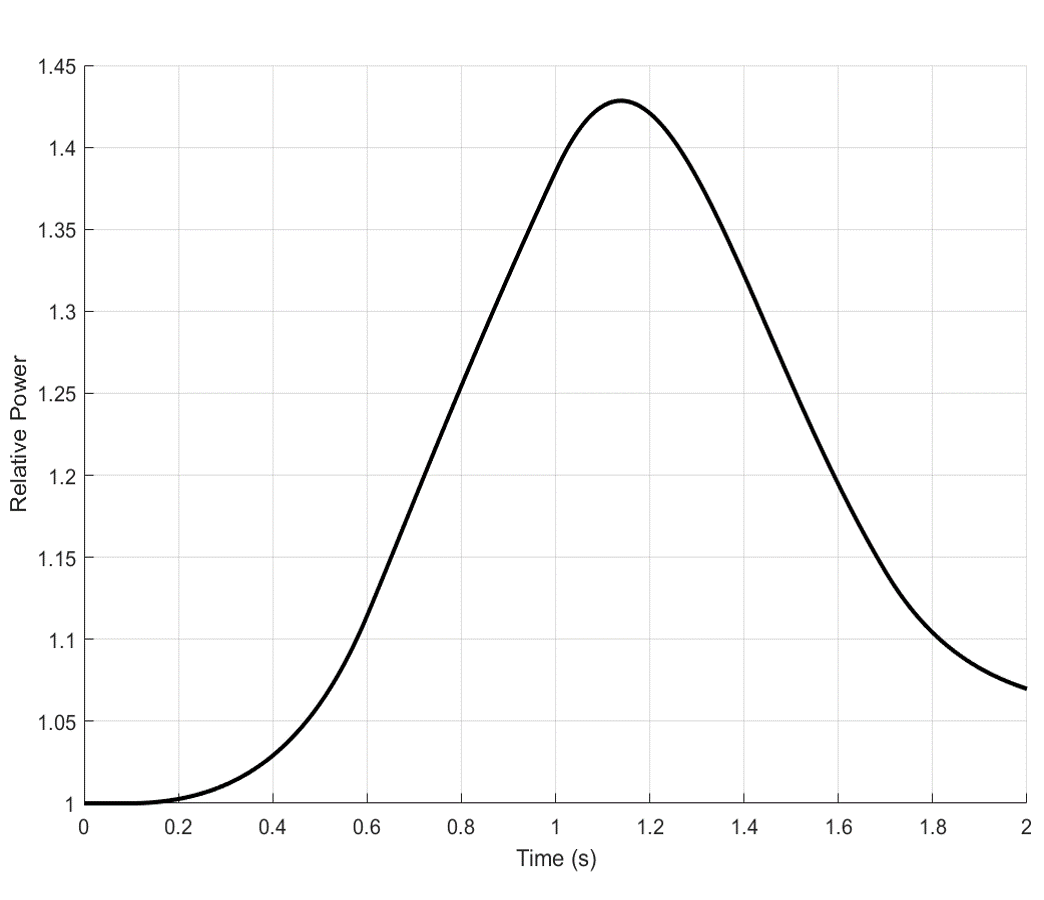
\includegraphics[width=\linewidth]{\FiguresDir/1D_power_base.png}
\caption{Baseline total power level for the 1D slab test case}
\label{fig:1D_power}
\end{center}
\end{figure}

\begin{figure}[!htbp]
\begin{center}
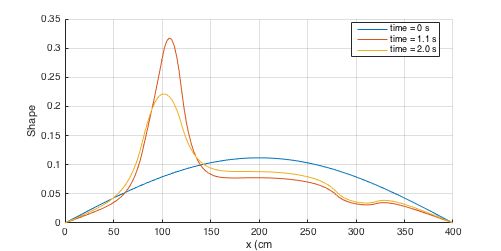
\includegraphics[width=\linewidth]{\FiguresDir/1D_shape.png}
\caption{Flux profile of 1D slab at various times}
\label{fig:1D_shape}
\end{center}
\end{figure}

\subsection{IQS Iteration Convergence}

IQS, as previously stated, is a system of nonlinear equations between shape and amplitude. These equations needed to be iterated to numerically converge to an accurate solution.  \sct{sect:iter} describes various iteration techniques for fixed-point and Newton schemes. \fig{fig:iter} shows the number of fixed-point iterations required for a $10^{-11}$ tolerance over the transient. The criteria listed in the legend are described as:
\begin{enumerate}
\item $L^{\infty} \rightarrow$ \eqt{eq:shape_Linf}
\item $L^{2} \rightarrow$ \eqt{eq:shape_L2}
\item Reactivity $\rightarrow$ \eqt{eq:rho_conv}
\item Amplitude $\rightarrow$ \eqt{eq:p_conv}
\item K criteria $\rightarrow$ \eqt{eq:K_conv}
\item All properties $\rightarrow$ \eqtss{eq:rho_conv}{eq:K_conv}
\end{enumerate}
This plot shows that 1-4 have approximately the same convergence behavior, but the K criteria converges to a certain error. \fig{fig:iter_err} shows the resulting error the K criteria converges to for different points of rescaling the shape. The rescaling is described by \eqt{eq:shape_scale}. Rescaling shape more frequently helps the error.  However, rescaling every iteration is somewhat artificial because it does not consider changes spatially. Regardless, an error of $~10^{-5}$ is quite large and it is expected that the magnitude is due to the explicit treatment of precursors (\eqt{eq:dnp_theta}). Switching to an analytical elimination (\eqt{eq:dnp_an}) does not converge as well, but the error is much smaller, seen in \fig{fig:iter_err_an}.

\begin{figure}[!htbp]
\centering
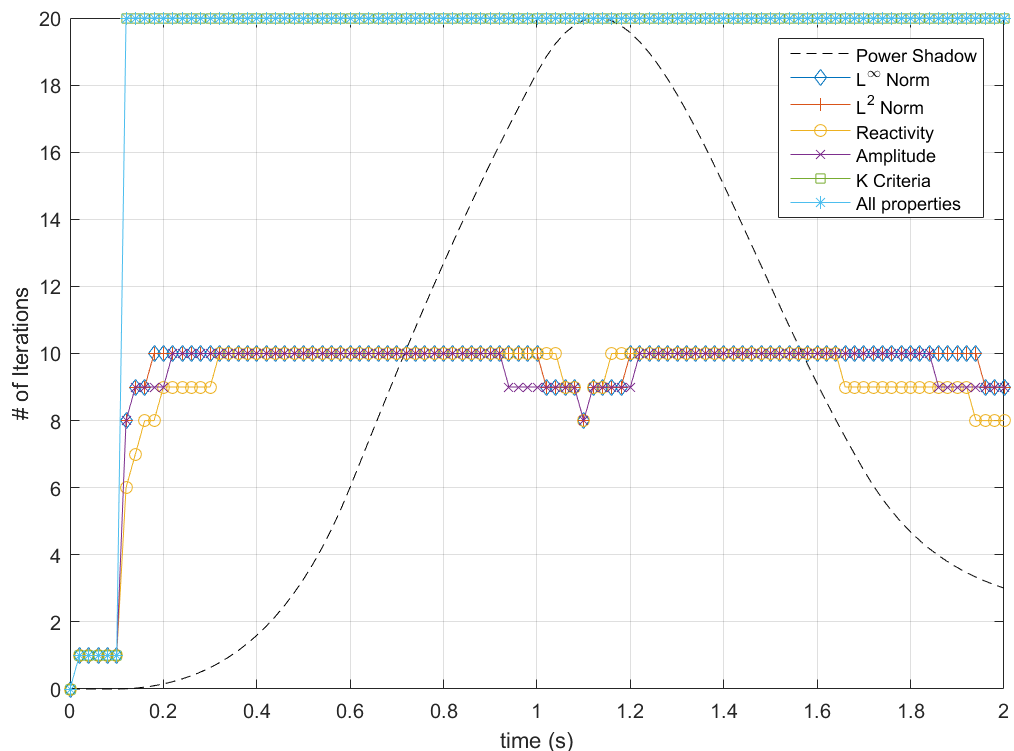
\includegraphics[width=0.75\linewidth]{\FiguresDir/iter_renorm.png}
\caption{\# of iterations for various convergence criteria, tolerance$=10^{-11}$, max iterations$=20$}
\label{fig:iter}
\end{figure}

\begin{figure}[!htbp]
\centering
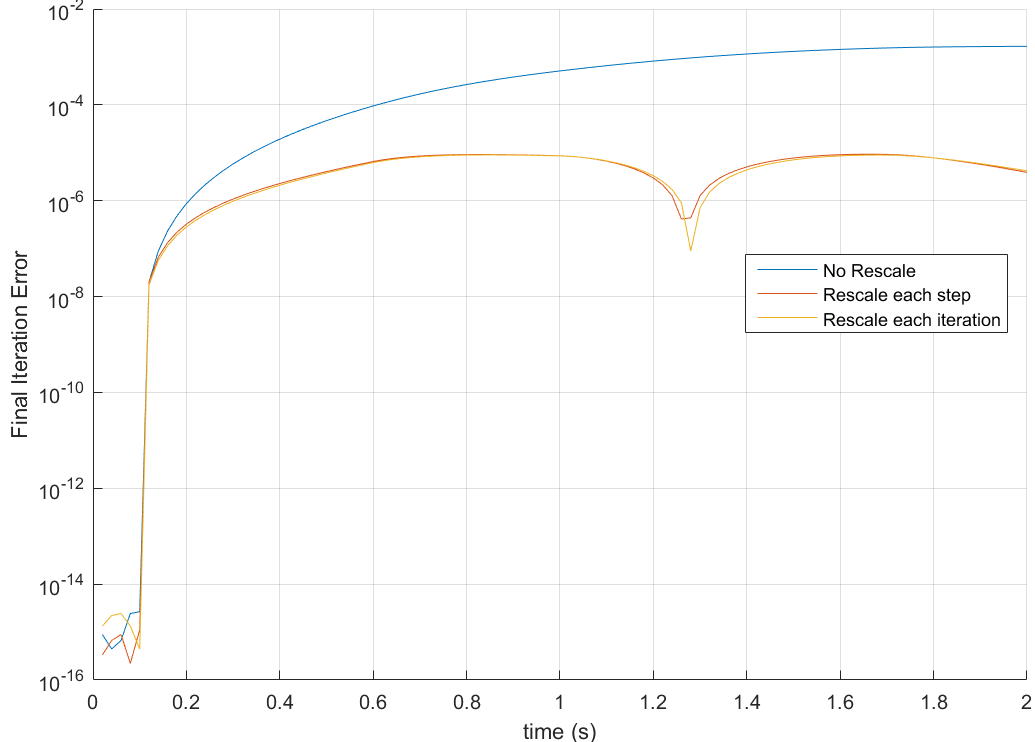
\includegraphics[width=0.75\linewidth]{\FiguresDir/iter_error.png}
\caption{Final iteration error for K convergence criteria}
\label{fig:iter_err}
\end{figure}

\begin{figure}[!htbp]
\centering
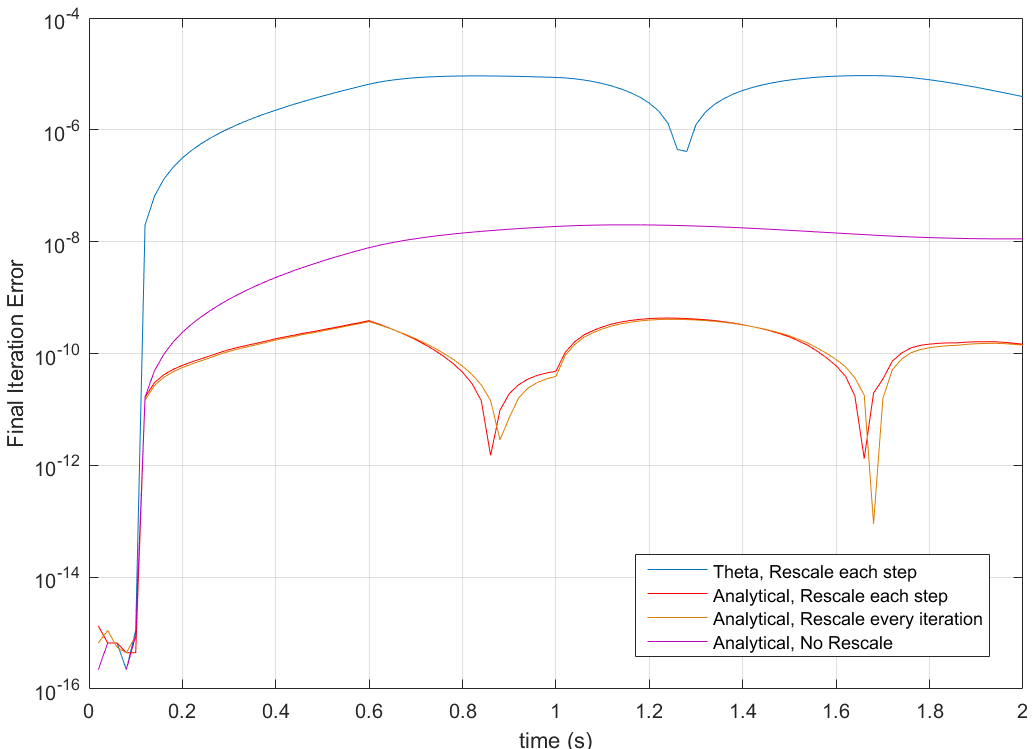
\includegraphics[width=0.75\linewidth]{\FiguresDir/iter_error_an.png}
\caption{Final iteration error for K convergence criteria with analytical precursor elimination}
\label{fig:iter_err_an}
\end{figure}


\subsection{Time Step Convergence}

Time step convergence analysis involves evaluating a problem with various refinements in step size and comparing the resulting errors with the time step size. Plotting error versus $\Delta t$ on a log-scale should produce a relatively strait line with a slope equal to the order of the time discretization method. In order to evaluate the performance and error convergence of IQS, the slab was simulated with varying time discretization methods and time step sizes.  \fig{fig:1D_conv} shows these convergence plots of five different discretization methods for implicit discretization, IQS, and IQS P-C.  These plots were generated from the results using the MATLAB prototype program.  The plots show that IQS and IQS P-C are convergent through fourth order BDF.  Third order SDIRK did not show third order convergence, but, through extensive testing, SDIRK shows non-convergent behavior for too stiff of problems.  

There are higher discretization order that can be tested, but most practical application do not go beyond second order.  This paper shows an analysis of the first publicized application of IQS with higher than second order discretization, which exposed unforeseen properties of IQS.  When using higher order techniques, the interpolation of PRKE parameters and shape for precursor integration become important to consider.  Every other application that was investigated linearly interpolates parameters for the PRKE evaluation.  Similarly, the shape used for the integration of the ODE for the precursors needs to have higher order interpolation to preserve high order error convergence.  This interpolation was done using Lagragian and Hermite methods, both leading to successful convergence.

The 1D slab problem was also applied to the Rattlesnake implementation of IQS.  \fig{fig:1D_conv_Rat} shows the error convergence for implicit Euler and BDF2 discretization of the three methods.  The results differ slightly from the prototype, especially in the fact that IQS P-C performs better than IQS.  Since Rattlesnake uses a PJFNK solver for the FEM model, number of time steps isn't strictly proportional to the execution time.  \fig{fig:1D_conv_lin} shows the error of the three methods as compared to the number of linear GMRES iterations, which is a better mark for comparison in computation time.  This figure shows that IQS performs worse than implicit discretization for most time-step sizes, but IQS P-C performs significantly better.  This is due to the fact that IQS needs to iterate between amplitude and shape to resolve its nonlinearity.

\begin{figure}[!htbp]
\centering
\begin{subfigure}[b]{0.49\textwidth}
\centering
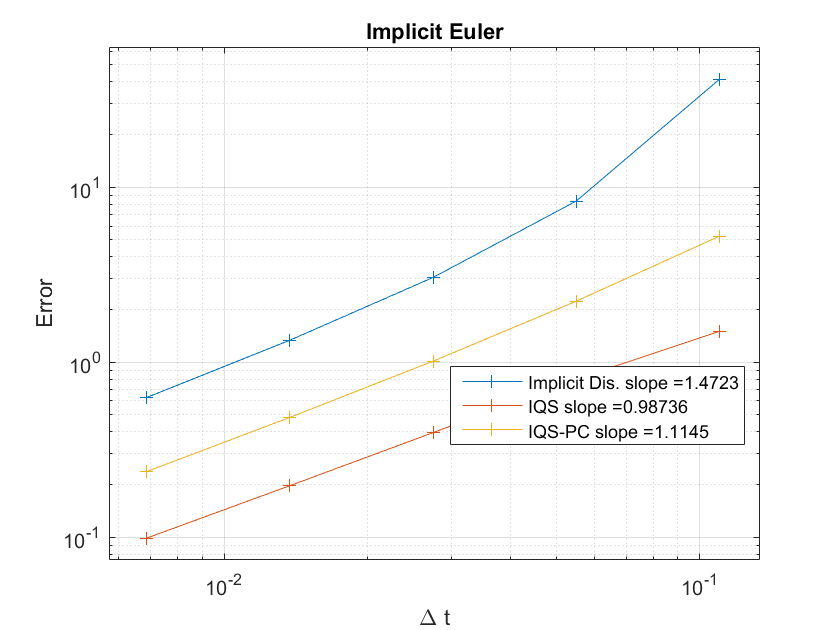
\includegraphics[width=\linewidth]{\FiguresDir/1D_conv_IE.png}
\caption{Implicit Euler}
\end{subfigure}
\begin{subfigure}[b]{0.49\textwidth}
\centering
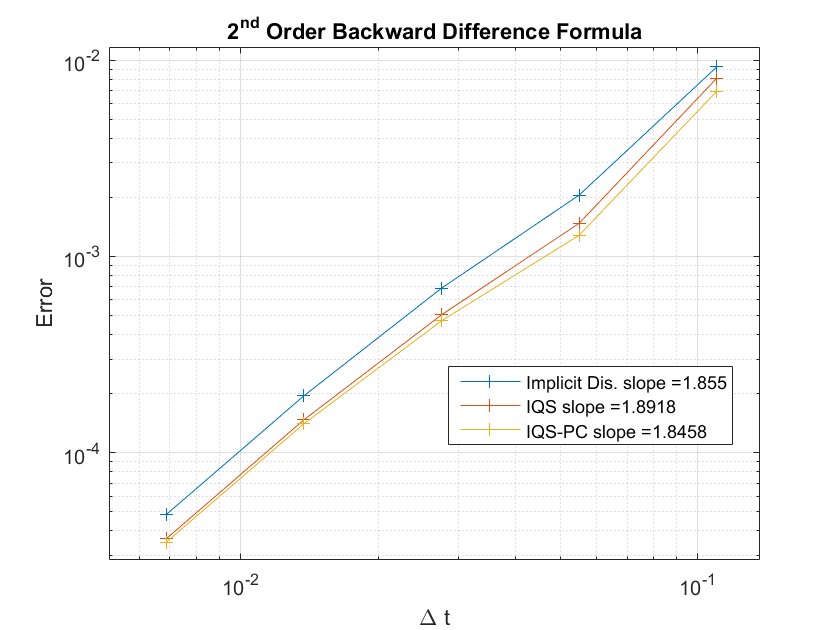
\includegraphics[width=\linewidth]{\FiguresDir/1D_conv_BDF2.png}
\caption{BDF2}
\end{subfigure}
\begin{subfigure}[b]{0.49\textwidth}
\centering
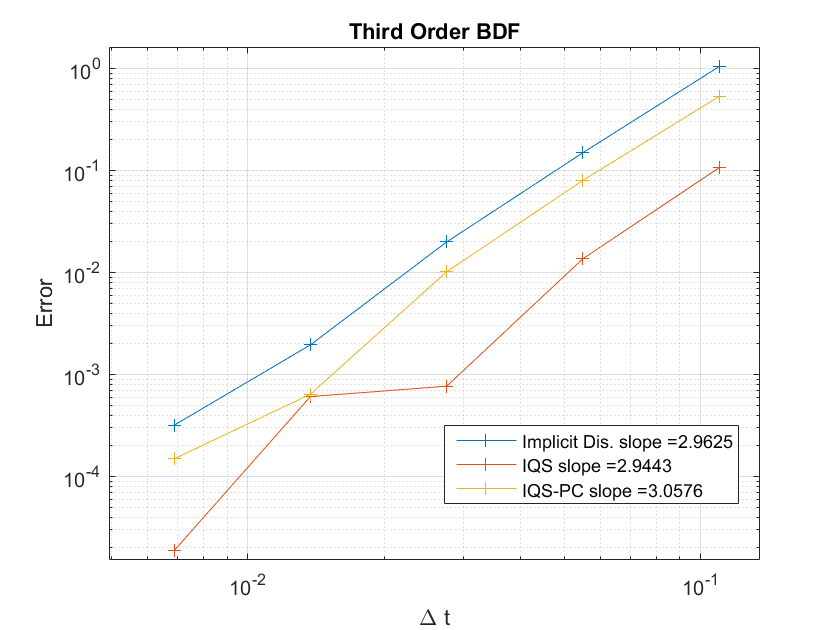
\includegraphics[width=\linewidth]{\FiguresDir/1D_conv_BDF3.png}
\caption{BDF3}
\end{subfigure}
\begin{subfigure}[b]{0.49\textwidth}
\centering
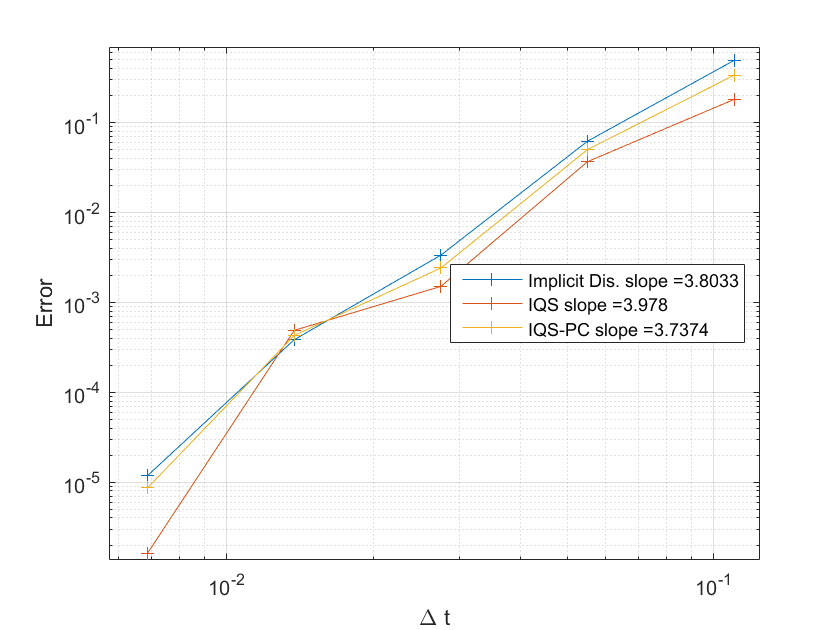
\includegraphics[width=\linewidth]{\FiguresDir/1D_conv_BDF4.png}
\caption{BDF4}
\end{subfigure}
\begin{subfigure}[b]{0.49\textwidth}
\centering
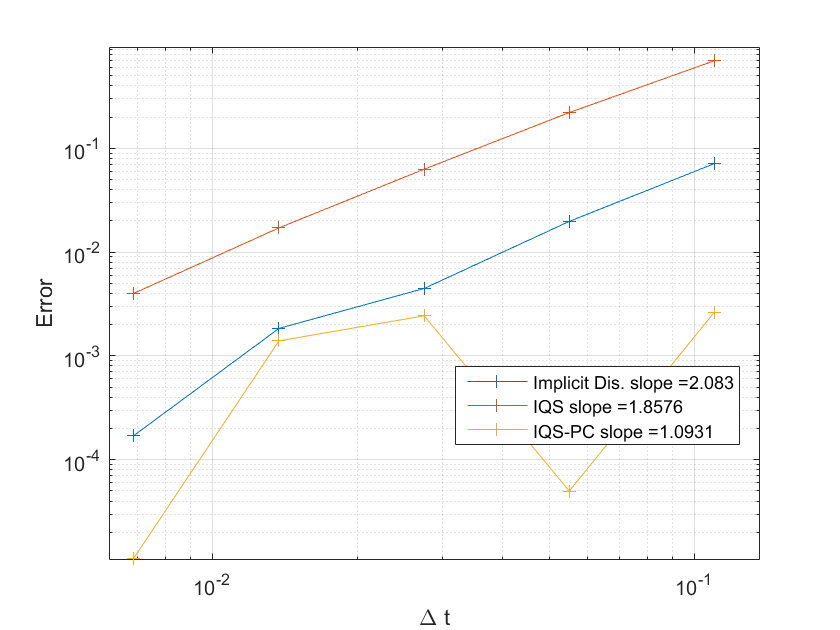
\includegraphics[width=\linewidth]{\FiguresDir/1D_conv_SDIRK33.png}
\caption{SDIRK33}
\end{subfigure}
\caption{Error convergence plots of implicit discretization, IQS, and IQS P-C with various time discretization schemes}
\label{fig:1D_conv}
\end{figure}

\begin{figure}[!htbp]
\begin{center}
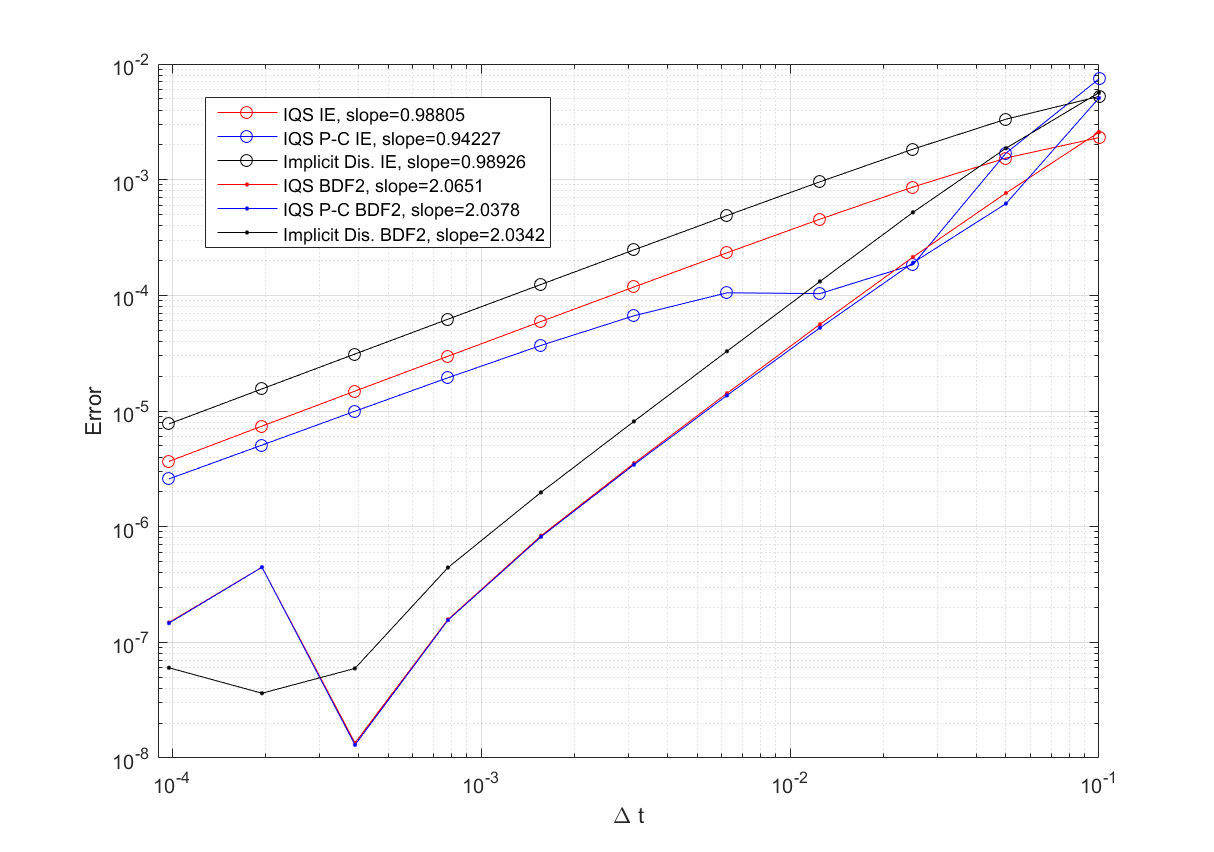
\includegraphics[width=0.75\linewidth]{\FiguresDir/1D_conv_Rat.png}
\caption{Error convergence plots of implicit discretization, IQS, and IQS P-C from Rattlesnake implementation}
\label{fig:1D_conv_Rat}
\end{center}
\end{figure}

\begin{figure}[!htbp]
\begin{center}
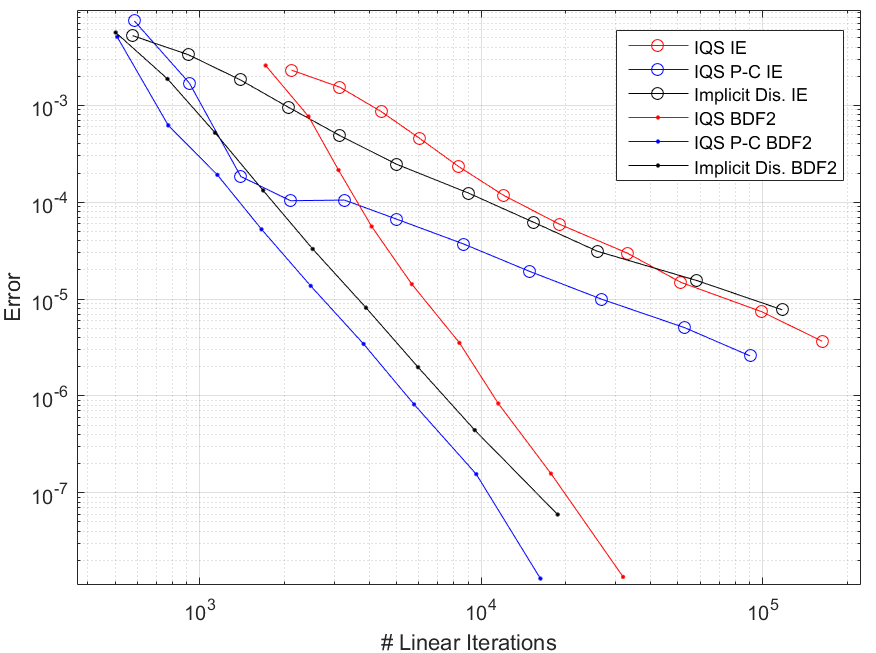
\includegraphics[width=0.75\linewidth]{\FiguresDir/1D_conv_lin.png}
\caption{Error convergence plots of implicit discretization, IQS, and IQS P-C vs. number of GMRES iterations}
\label{fig:1D_conv_lin}
\end{center}
\end{figure}

\pagebreak
\section{TWIGL Benchmark}

This benchmark problem originates from the Argonne National Lab Benchmark Problem Book \cite{ANL_BPB}.  It is a 2D, 2-group reactor core model with no reflector region shown in \fig{fig:TWIGL_reg} \cite{TWIGL_benchmark}.  This example is meant to be of progressive complexity from the previous example.  The transient of this reactor is very geometrically symmetrical with very little temporal shape change.  Therefore, IQS is expected to perform significantly better than the implicit discretization method.  \tbl{tab:TWIGL_mat} shows the material properties of each fuel region and the ramp perturbation of Material 1.

\begin{figure}[!htbp]
\begin{center}
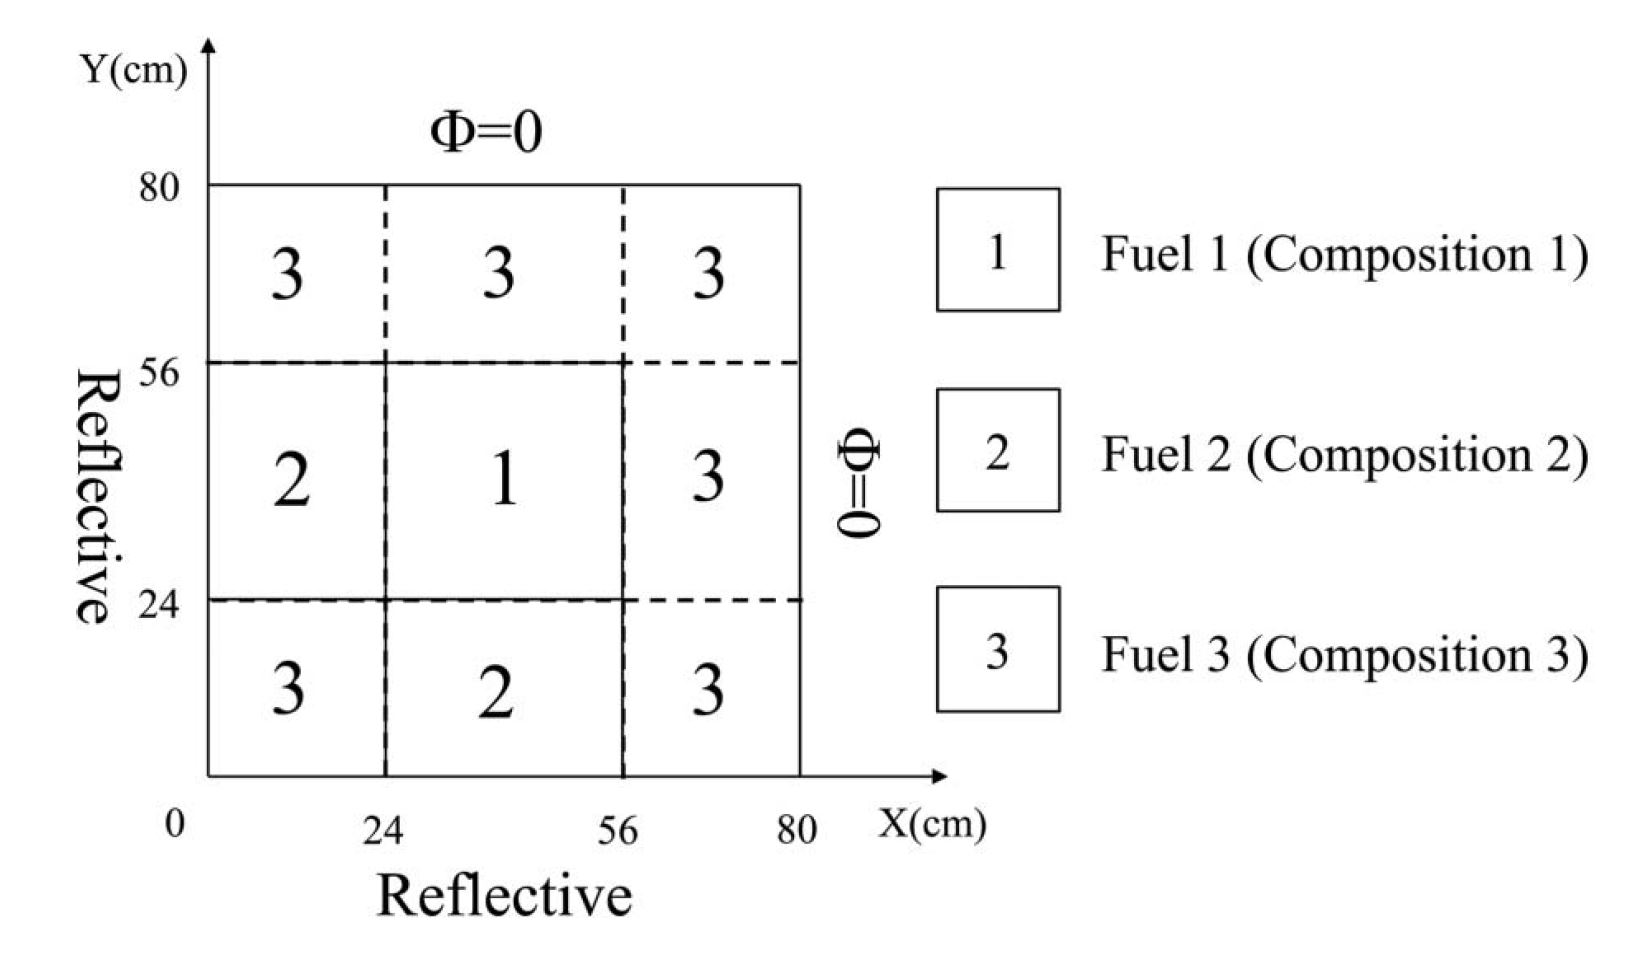
\includegraphics[width=0.75\textwidth]{\FiguresDir/TWIGL_regions.jpg}
\caption{TWIGL benchmark problem description}
\label{fig:TWIGL_reg}
\end{center}
\end{figure}
\begin{table}[!htbp]
\begin{center}
\caption{TWIGL benchmark material properties and slope perturbation}
\label{tab:TWIGL_mat}
\begin{tabular}{llllllll}
\hline
  &  &  &  &  &  &  \multicolumn{2}{c}{$\underline{\Sigma_s (cm^{-1})} $} \\
Material & Group & $D (cm)$ & $\Sigma_a (cm^{-1})$ & $\nu\Sigma_f (cm^{-1})$ & $\chi$ & $g \rightarrow 1$ & $g \rightarrow 2$ \\
\hline
1 & 1 & 1.4 & 0.010 & 0.007 & 1.0 & 0.0 & 0.01 \\
  & 2 & 0.4 & 0.150 & 0.200 & 0.0 & 0.0 & 0.00  \\
2 & 1 & 1.4 & 0.010 & 0.007 & 1.0 & 0.0 & 0.01  \\
  & 2 & 0.4 & 0.150 & 0.200 & 0.0 & 0.0 & 0.00  \\
3 & 1 & 1.3 & 0.008 & 0.003 & 1.0 & 0.0 & 0.01  \\
  & 2 & 0.5 & 0.050 & 0.060 & 0.0 & 0.0 & 0.00  \\
\hline
  & $\nu$ & $v_1 (cm/s)$ & $v_2 (cm/s)$ & $\beta$ & $\lambda (1/s)$ &   &   \\
\hline
  & 2.43 & 1.0E7 & 2.0E5 & 0.0075 & 0.08 &   &   \\
\hline
 \multicolumn{8}{l}{\footnotesize Material 1 ramp perturbation:} \\
\multicolumn{8}{l}{\footnotesize $\Sigma_{a,2}(t)=\Sigma_{a,2}(0) \times (1-0.11667t) \quad t \leq 0.2 s$} \\
\multicolumn{8}{l}{\footnotesize $\Sigma_{a,2}(t)=\Sigma_{a,2}(0) \times (0.97666t) \quad t > 0.2 s$} \normalsize
\end{tabular}
\end{center}
\end{table}

\subsection{TWIGL Convergence Analysis}


Figs. \ref{fig:TWIGL_power} and \ref{fig:TWIGL_plots} show the IQS  solution as compared with the implicit discretization solution.  It is important to note the IQS shape plot is scaled differently than the Brute Force flux plot (\fig{fig:TWIGL_plots}) because the amplitude term is not included, but the gradients of colors is comparable. These plots show that IQS is consistent in more complex, higher dimensional problems in Rattlesnake. These plots also serve to illustrate that IQS has a much more accurate solution, even at a significantly larger time step than the implicit discretization. In order to demonstrate asymptotic convergence of IQS, implicit Euler (IE) and second order BDF (BDF2) were applied to the TWIGL simulation. \fig{fig:TWIGL_conv} plots the error convergence of IQS and the implicit discretization methods.  The curves show the impressive convergence of IQS for the highly transient TWIGL example. The slope indicated in the legend are the linear slope of curves on the log plot, these slopes should be similar to the order of the method (1 for IE and 2 for BDF2).  IQS shows a increased order because the PRKE is performing much of accuracy convergence and it is computed using SDIRK33, a third order method.

\begin{figure}[!htbp]
\centering
\begin{subfigure}[!htbp]{0.49\textwidth}
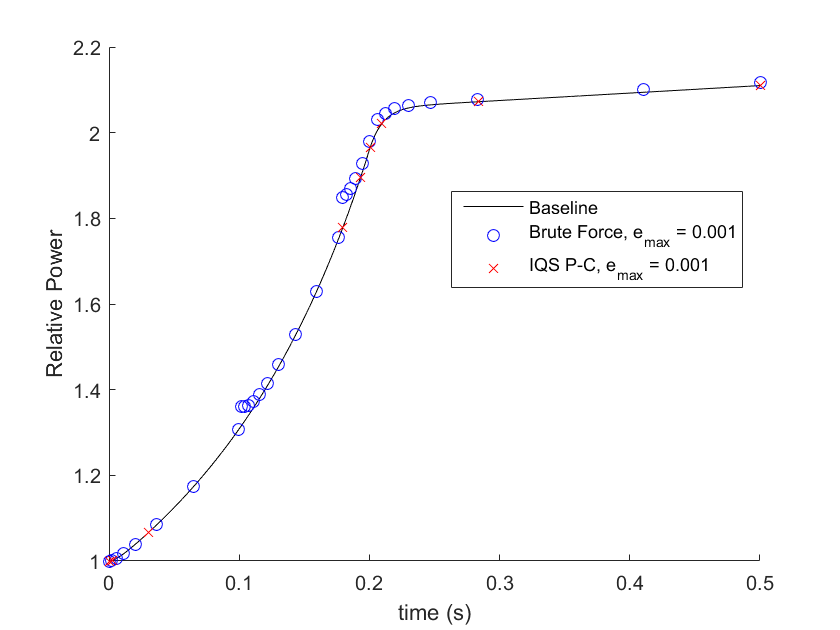
\includegraphics[width=\textwidth]{\FiguresDir/TWIGL_power_plot.png}
\caption{Power profile for entire transient}
\end{subfigure}
\begin{subfigure}[!htbp]{0.49\textwidth}
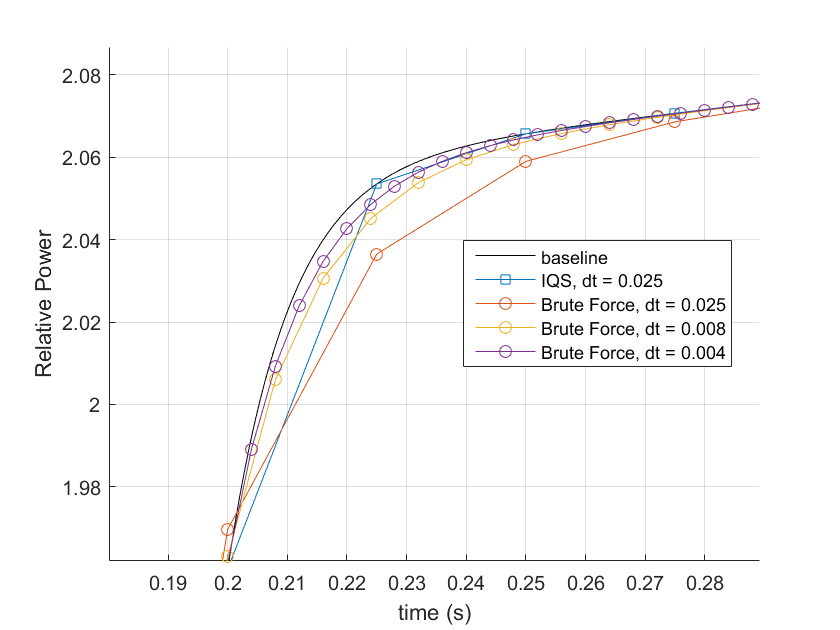
\includegraphics[width=\textwidth]{\FiguresDir/TWIGL_power_plot2.png}
\caption{Power at cusp of profile}
\end{subfigure}
\caption{Power level comparison of TWIGL Benchmark}
\label{fig:TWIGL_power}
\end{figure}

\begin{figure}[!htbp]
\begin{center}
\begin{subfigure}[!htbp]{0.4\textwidth}
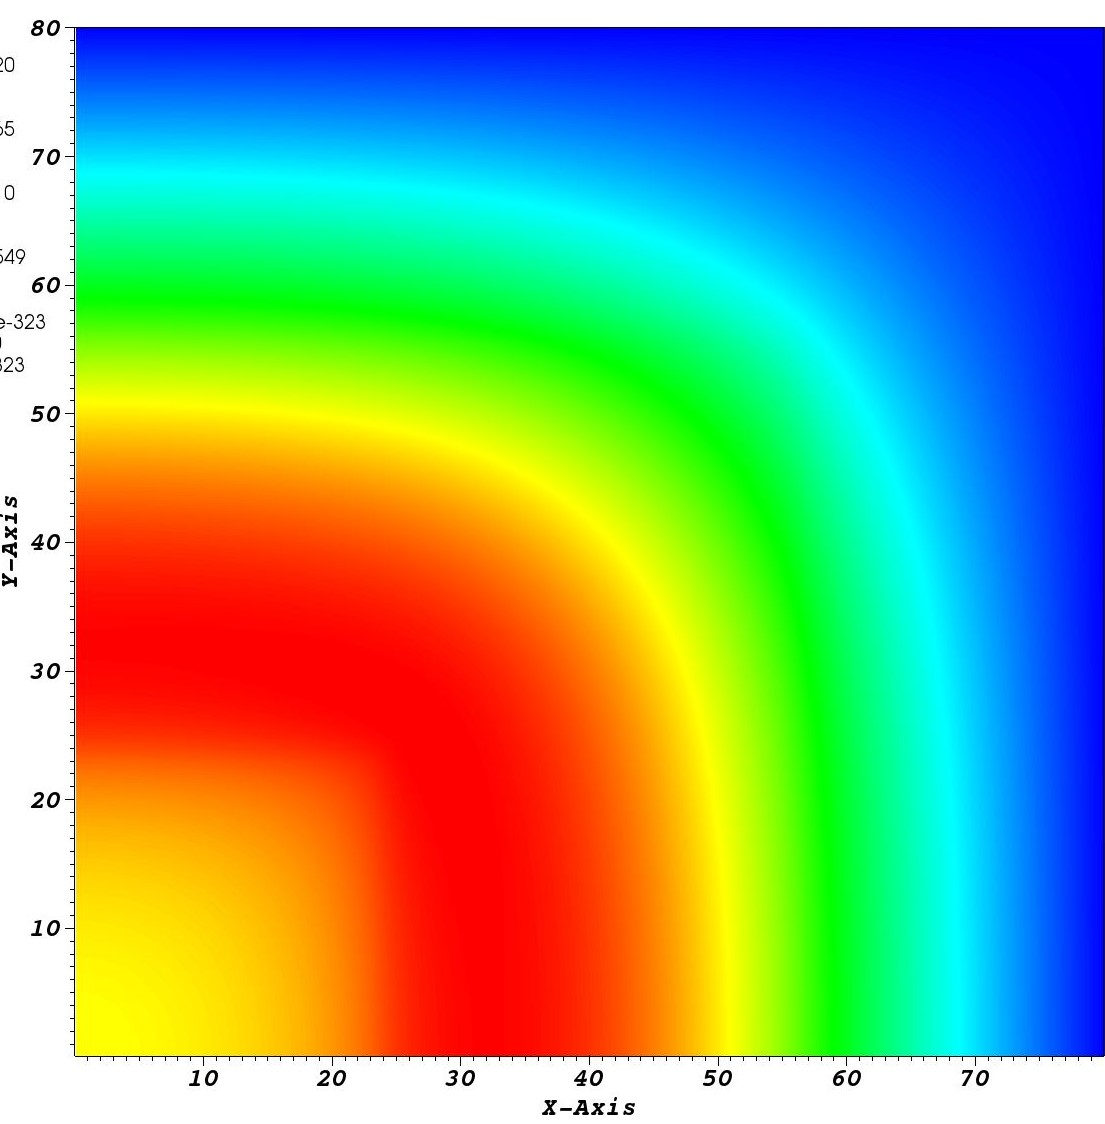
\includegraphics[width=\textwidth]{\FiguresDir/ndiff_ramp_flux.jpg}
\caption{Implicit Discretization flux}
\end{subfigure}
\quad
\begin{subfigure}[!htbp]{0.4\textwidth}
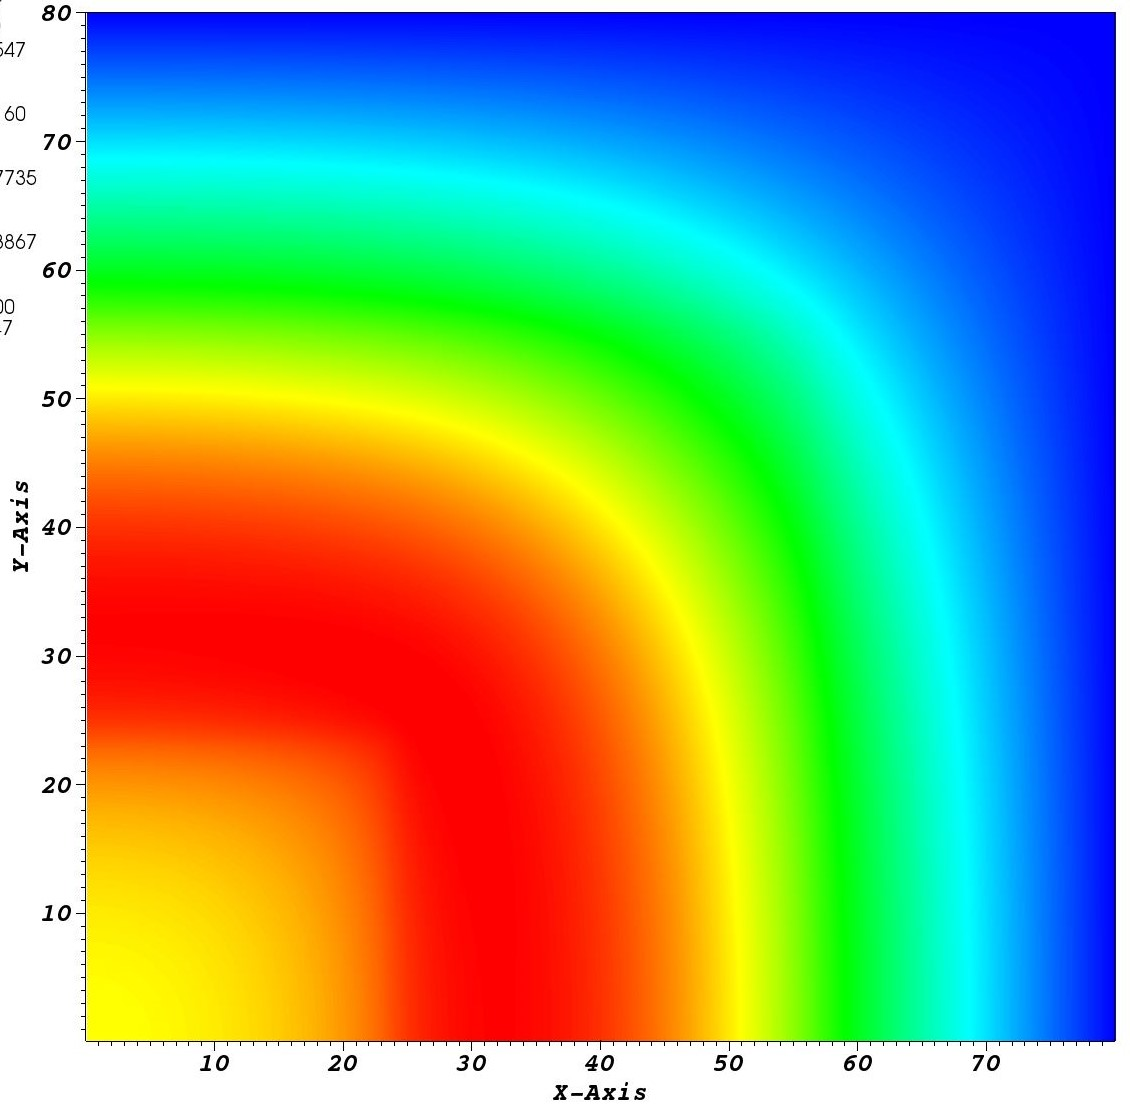
\includegraphics[width=\textwidth]{\FiguresDir/iqs_ramp_shape.jpg}
\caption{IQS Shape}
\end{subfigure}
\caption{TWIGL Benchmark flux/shape comparison at $t=0.2$}
\label{fig:TWIGL_plots}
\end{center}
\end{figure}

\begin{figure}[!htbp]
\centering
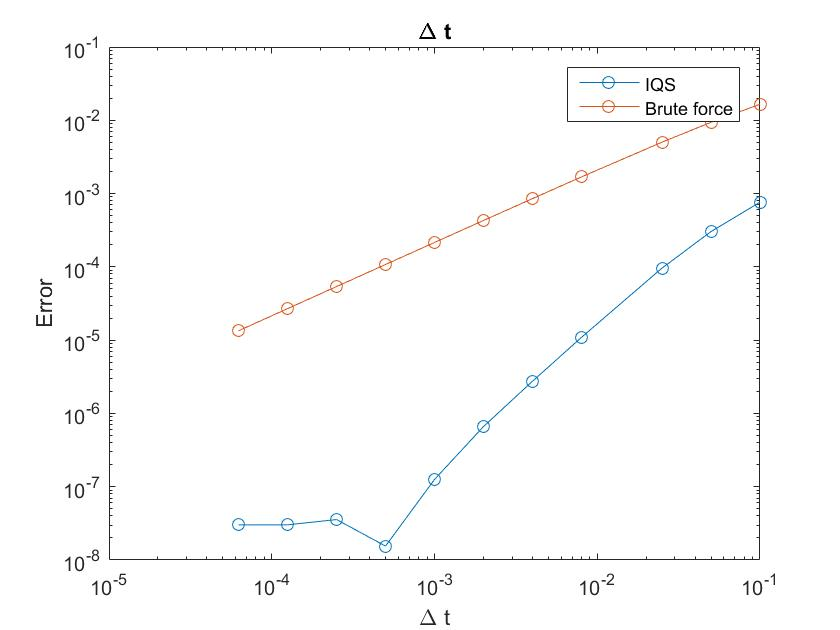
\includegraphics[height=3in]{\FiguresDir/TWIGL_convergence.jpg}
\caption{Error convergence comparison of TWIGL Benchmark}
\label{fig:TWIGL_conv}
\end{figure}

\subsection{TWIGL with Step Doubling Time Adaptation}

\tbl{tab:TWIGLdt2} and \fig{fig:TWIGL_power_dt2} show the results for TWIGL with time adaptation.  The results show that both IQS methods perform exceptionally well compared to implicit discretization.  It also shows that traditional IQS performed better with large $e_{tol}$, while IQS P-C was better with smaller $e_{tol}$.

\begin{table}[!htbp]
\begin{center}
\caption{TWIGL step doubling results}
\label{tab:TWIGLdt2}
\resizebox{\textwidth}{!}{
\begin{tabular}{|l|l|l|l|l|l|l|l|l|l|l|}
\hline
  &  & \multicolumn{3}{|c|}{Implicit Discretization} & \multicolumn{3}{|c|}{IQS} & \multicolumn{3}{|c|}{IQS P-C} \\
\hline
Test & $e_{tol}$ & Error & Steps & Solves & Error & Steps & Solves & Error & Steps & Solves \\
\hline
1 &	0.05    &	0.00012677 &	9   &	29  &	0.03380433 &	4   &	20   &	0.00323100 &	4  &	9   \\
2 &	0.01    &	3.5555e-05 &	11  &	35  &	0.00166991 &	5   &	40   &	0.00263068 &	5  &	12  \\
3 &	0.005   &	4.0364e-05 &	11  &	31  &	0.00886584 &	5   &	40   &	0.00160486 &	6  &	21  \\
4 &	0.001   &	0.00294822 &	33  &	122 &	0.02976305 &	5   &	36   &	1.7527e-05 &	10 &	35  \\
5 &	0.0005  &	0.00099778 &	39  &	131 &	0.00143781 &	6   &	55   &	1.4185e-05 &	16 &	74  \\
6 &	0.0001  &	0.00019510 &	78  &	236 &	0.00016175 &	8   &	65   &	6.2903e-06 &	19 &	78  \\
7 &	5.0e-05 &	0.00018372 &	112 &	342 &	6.0328e-05 &	12  &	163  &	1.5247e-06 &	24 &	92  \\
8 &	1.0e-05 &	8.0564e-05 &	263 &	794 &	7.7103e-05 &	379 &	5729 &	9.8321e-07 &	48 &	210 \\
\hline

\end{tabular}}
\end{center}
\end{table}

\begin{figure}[!htbp]
\centering
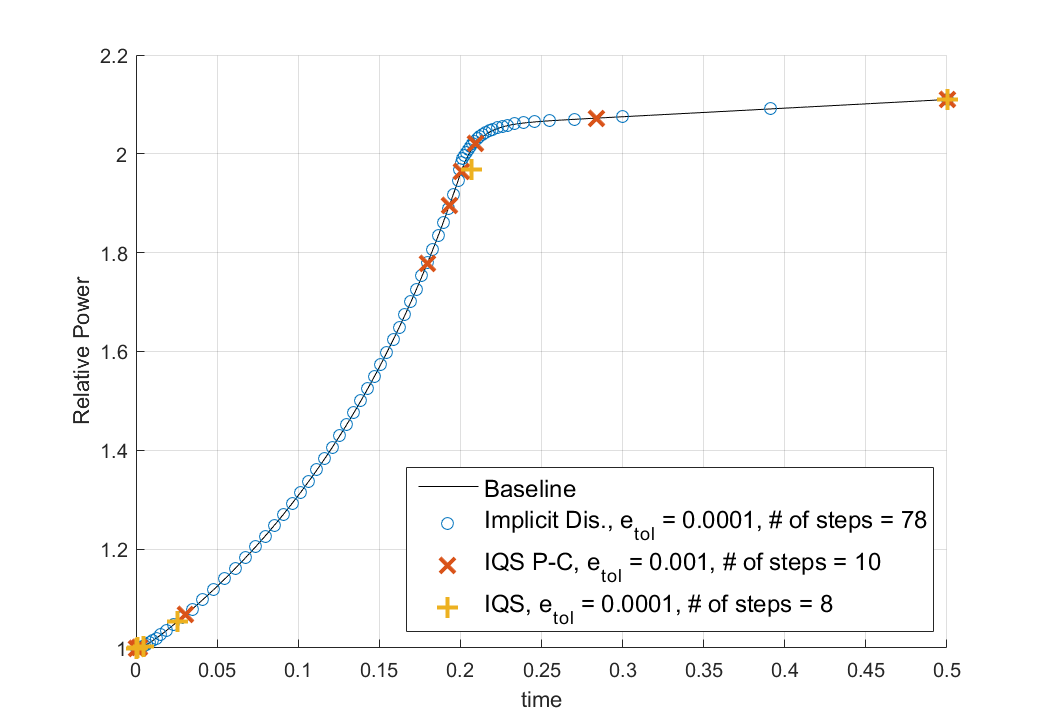
\includegraphics[width=0.8\linewidth]{\FiguresDir/TWIGL_power_plot_dt2.png}
\caption{Power level comparison of TWIGL Benchmark with time adaptation}
\label{fig:TWIGL_power_dt2}
\end{figure}

%\pagebreak
%\section{C5G7-TD Benchmark}
%
%The C5G7 benchmark is a MOX fueled, pressurized water reactor (PWR) minicore configuration. The C5G7 geometry depicted in Fig. \ref{fig:c5g7-2D} comprises a 2-by-2 array of UO$_2$ and MOX assemblies surrounded by moderator. In Fig. \ref{fig:c5g7-2D} vacuum and reflective boundary conditions are denoted by V and R, respectively. The fuel pins are not homogenized, each pin cell is comprised of a fuel pin, fission chamber, or guide tube surrounded by moderator as depicted in Fig. \ref{fig:c5g7-pincell}. The cladding and gap are homogenized into the fuel and are not explicitly modeled. Each assembly is made up of a regular 17-by-17 grid of pin cells.
%Seven energy-group cross sections for the seven material regions are given in \cite{c5g7}. The energy group boundaries are provided in Table \ref{tab:c5g7-ebounds}; three of the seven energy groups are fast, four are thermal.
%
%\begin{figure}[!htpb]
%\begin{center}
%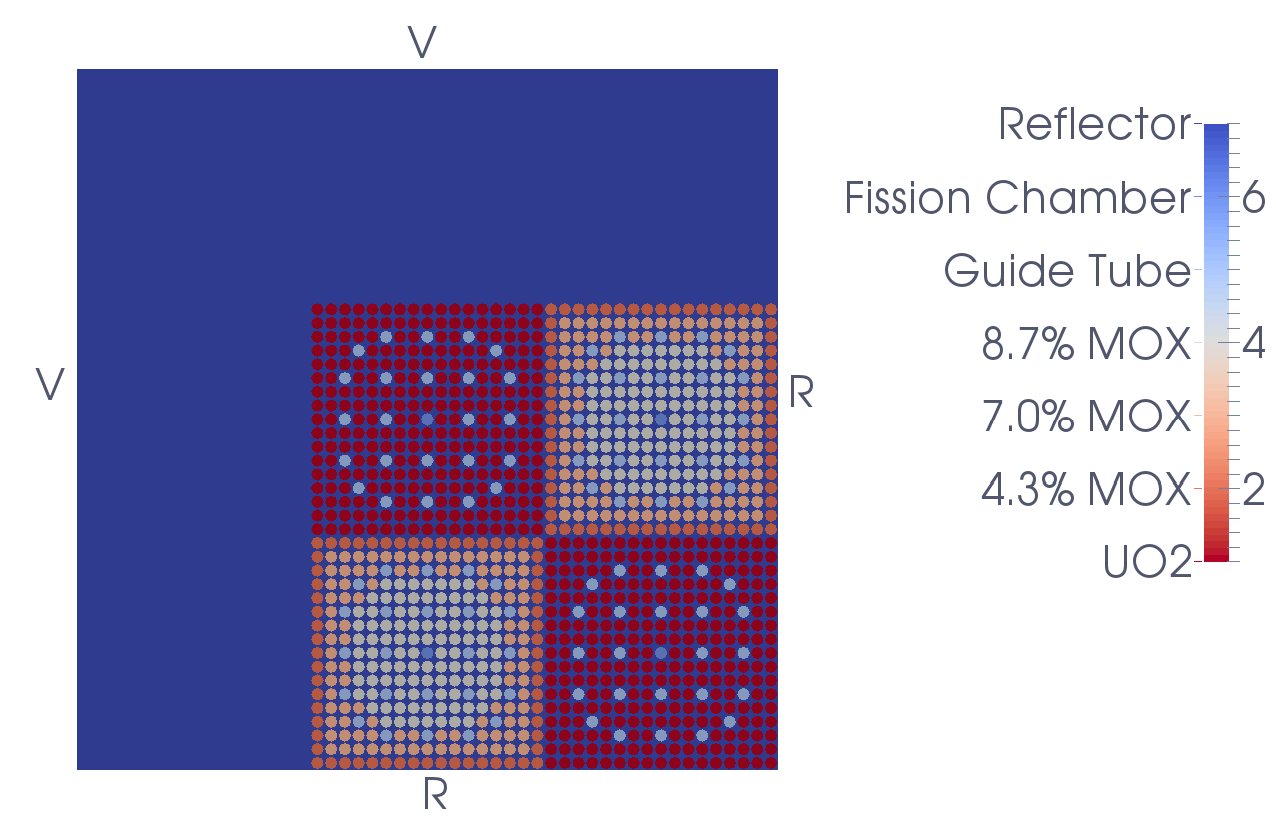
\includegraphics[width=\linewidth]{\FiguresDir/C5G7-2D.png}
%\end{center}
%\caption{Geometry of the two-dimensional C5G7 benchmark problem. Boundary conditions are vacuum (V) or reflective (R).}
%\label{fig:c5g7-2D}
%\end{figure}
%
%\begin{figure}[!htpb]
%\begin{center}
%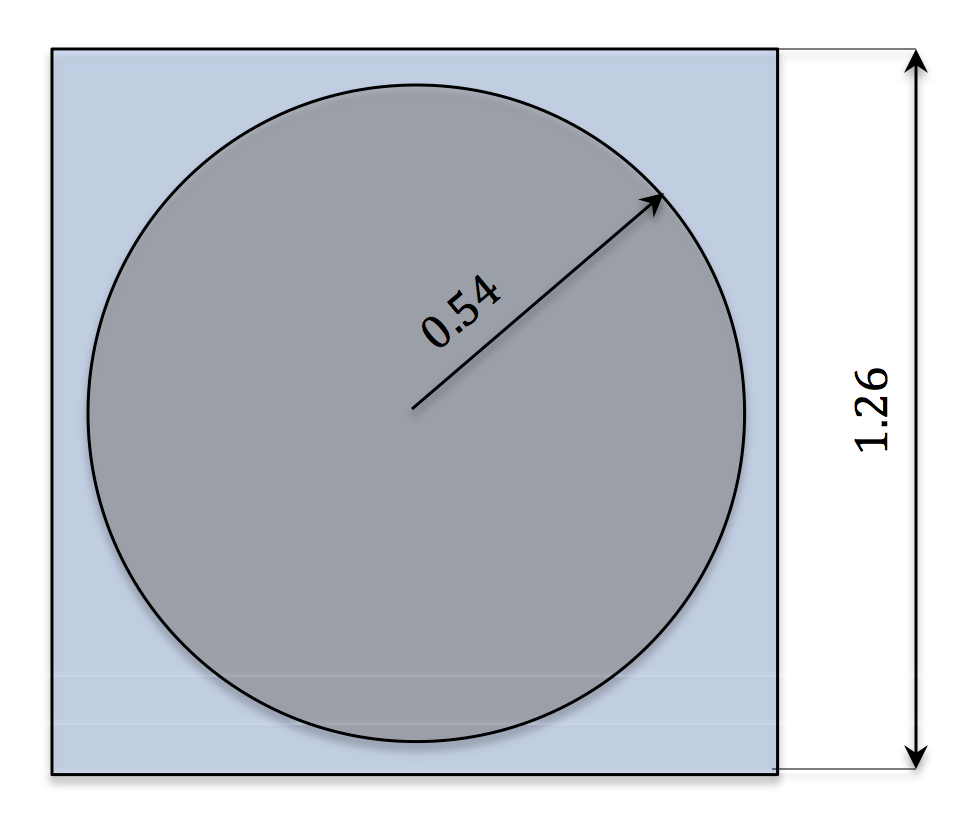
\includegraphics[width=0.5\linewidth]{\FiguresDir/C5G7-pincell.png}
%\end{center}
%\caption{Geometry of a C5G7 pin-cell.}
%\label{fig:c5g7-pincell}
%\end{figure}
%
%\begin{table}[!htpb]
%\centering
%\caption{Energy group boundaries for C5G7 MOX benchmark.}
%\label{tab:c5g7-ebounds}
%\begin{tabular}{c c}
%\hline
%Group & Upper Energy\\
%\hline
% 1&20 MeV  \\
% 2&1 MeV  \\
% 3&500 keV  \\
% 4&3 eV  \\
% 5&0.625 MeV  \\
% 6&0.1 MeV  \\
%71&0.02 MeV  \\
%\hline
%\end{tabular}
%\end{table}
%
%\pagebreak
%\section{LMW Benchmark?}


%%%%%%%%%%%%%%%%%%%%%%%%%%%%%%%%%%%%%%%%%%%%%%%%%%%
%
%  New template code for TAMU Theses and Dissertations starting Fall 2016.
%
%  Author: Sean Zachary Roberson
%	 Version 3.16.09
%  Last updated 9/12/2016
%
%%%%%%%%%%%%%%%%%%%%%%%%%%%%%%%%%%%%%%%%%%%%%%%%%%%
%%%%%%%%%%%%%%%%%%%%%%%%%%%%%%%%%%%%%%%%%%%%%%%%%%%%%%%%%%%%%%%%%%%%%%
%%                           SECTION IV
%%%%%%%%%%%%%%%%%%%%%%%%%%%%%%%%%%%%%%%%%%%%%%%%%%%%%%%%%%%%%%%%%%%%%



\chapter{DYNAMICS EXAMPLES \label{sect:dyn}}

Reactor dynamics is the study of the time-dependent behavior of reactors as an entire system. This study includes the physical nature of neutrons and their feedback with power generation.  This feedback includes coupling with other physical properties such as temperature, fluids, material dynamics, etc.  This section describes several dynamics examples, including the LRA benchmark and two TREAT experiments.  These examples are of increased complexity from the kinetics examples of \sct{sect:kin}.  This section also analyzes IQS's performance with these, which is vital for verification of IQS in real-world problems.

\section{LRA Benchmark}

The LRA benchmark is a two-dimensional, two-group neutron diffusion problem with adiabatic heat-up and Doppler feedback in thermal reactor \cite{ANL_BPB}.  It is a super prompt-critical transient.  To have better understanding on the cross sections given later, we present the equations here:
\begin{subequations}
\begin{align}
-\frac{1}{v_1} \frac{\partial \phi_1}{\partial t} &= -\div D_1 \grad\phi_1 + (\Sigma_{a,1} + \Sigma_{s, 1\rightarrow 2})\phi_1 - \nu(1-\beta)S_f  - \sum_{i=1}^2 \lambda_i C_i, \\
-\frac{1}{v_2} \frac{\partial \phi_2}{\partial t} &= -\div D_2 \grad\phi_1 + \Sigma_{a,2}\phi_2 - \Sigma_{s, 1\rightarrow 2}\phi_1, \\
S_f &= \sum_{g=1}^2 \Sigma_{f,g} \phi_g, \\
\frac{\partial C_i}{\partial t} &= \nu\beta_i f - \lambda_i C_i, \quad i=1,2, \\
\frac{\partial T}{\partial t} &= \alpha f, \label{eq:lra-temp} \\
\Sigma_{a,1} &= \Sigma_{a,1}(\vec{r}, t=0) \left[1+\gamma\left(\sqrt{T} - \sqrt{T_0}\right)\right], \\
P &= \kappa S_f,
\end{align}
\end{subequations}
where $\phi_1$, $\phi_2$ are the fast and thermal fluxes; $v_1, v_2$ are the averaged neutron velocities; $\Sigma_{a,1}, \Sigma_{a,2}$ are the absorption cross sections; $\Sigma_{s,1\rightarrow 2}$ is the fast-to-thermal scattering cross section; $\Sigma_{f,1}, \Sigma_{f,2}$ are the fission cross sections; $\nu$ is the averaged number of neutrons emitted per fission; $\beta_1, \beta_2$ are the delayed neutron precursor fractions and $\beta=\beta_1 + \beta_2$; $C_1, C_2$ are the delayed neutron precursor concentrations; $\lambda_1, \lambda_2$ are the decay constants of the delayed neutron precursors; $S_f$ is the fission reaction rate; $P$ is the power density; $T$ is the temperature; $\kappa$ is the averaged power released per fission; $\alpha$ is the combination of $\kappa$ and the specific heat capacity; $\gamma$ is the Doppler feedback coefficient; $T_0=T(\vec{r}, t=0)$.
The two-group diffusion equation are solved with zero flux boundary conditions on external surfaces, reflecting conditions at symmetry boundaries and steady state initial conditions which are obtained by solving
\begin{align}
-\div D_1 \grad\phi_1 + (\Sigma_{a,1} + \Sigma_{s, 1\rightarrow 2})\phi_1 &= \frac{1}{k}\sum_{g=1}^2 \nu\Sigma_{f,g}\phi_g, \\
-\div D_2 \grad\phi_1 + \Sigma_{a,2}\phi_2 =& \Sigma_{s, 1\rightarrow 2}\phi_1.
\end{align}
The eigenvalue $k$ is used to modify the fission cross section for the transient simulations with $\frac{1}{k}\Sigma_{f,g}, g=1,2$.  The initial flux distribution shall be normalized such that the averaged power density
\begin{align}
\bar{P} \equiv \frac{\int_{V_{core}} P(\vec{r}, t=0) d\vec{r}}{\int_{V_{core}} d\vec{r}},
\end{align}
where $V_{core}$ is the core region with fuels, is equal to $10^{-6} W\cdot cm^{-3}$.
The initial precursor concentrations are in equilibrium with the initial critical flux distribution.\\

The geometry is illustrated in~\fig{fig:lra-geometry}.\\
\begin{figure}[!htbp]
\centering
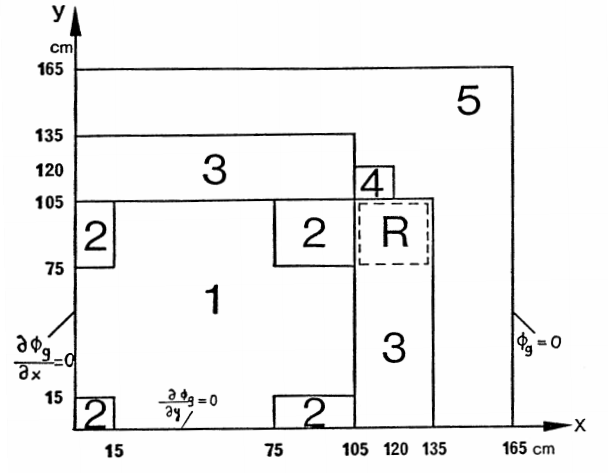
\includegraphics[width=0.8\linewidth]{\FiguresDir/lra.png}
\caption{LRA benchmark geometry with region assignment.}
\label{fig:lra-geometry}
\end{figure}

Initial two-group constants are presented in~\tbl{tab:lra-xs}.
$\nu$ is equal to 2.43.
Axial bulking $B^2 = 10^{-4}$ is applied for both energy groups.
Delayed neutron data are presented in~\tbl{tab:lra-dnp}.
All fuel materials have the same delayed neutron data.
Some scalar data are listed in~\tbl{tab:lra-scalar}.\\
\begin{table}[!htbp]
    \centering
    \caption{LRA benchmark initial two-group constants.\label{tab:lra-xs}}
    \resizebox{\textwidth}{!}{
      \begin{tabular}{|c|c|c|c|l|l|l|l|l|}
      \hline
             &                 & Group   & $D_g$      & $\Sigma_{a,g}$ & $\nu\Sigma_{f,g}$ & $\Sigma_{s,1\rightarrow 2}$ & $\chi_g$ & $v_g$              \\
      Region & Material        &       g & (cm)       &  ($cm^{-1}$)   &  ($cm^{-1}$)      &  ($cm^{-1}$)                &          & ($cm\cdot s^{-1}$) \\
      \hline
      1      & Fuel 1 with rod & 1       & 1.255      & 0.008252       & 0.004602          &                             & 1        & $3.0\times10^7$    \\
             &                 & 2       & 0.211      & 0.1003         & 0.1091            & 0.02533                     & 0        & $3.0\times10^5$    \\
      \hline
      2      & Fuel 1 without rod & 1    & 1.268      & 0.007181       & 0.004609          &                             & 1        & $3.0\times10^7$    \\
             &                    & 2    & 0.1902     & 0.07047        & 0.08675           & 0.02767                     & 0        & $3.0\times10^5$    \\
      \hline
      3      & Fuel 2 with rod & 1       & 1.259      & 0.008002       & 0.004663          &                             & 1        & $3.0\times10^7$    \\
             &                 & 2       & 0.2091     & 0.08344        & 0.1021            & 0.02617                     & 0        & $3.0\times10^5$    \\
      \hline
      4      & Fuel 2 without rod & 1    & 1.259      & 0.008002       & 0.004663          &                             & 1        & $3.0\times10^7$    \\
             &                    & 2    & 0.2091     & 0.073324       & 0.1021            & 0.02617                     & 0        & $3.0\times10^5$    \\
      \hline
      5      & Reflector        & 1      & 1.257      & 0.0006034      & -                 &                             & -        & $3.0\times10^7$    \\
             &                  & 2      & 0.1592     & 0.01911        & -                 & 0.04754                     & -        & $3.0\times10^5$    \\
      \hline
      \end{tabular}}
\end{table}

\begin{table}[!htbp]
    \centering
    \caption{LRA benchmark delayed neutron data.\label{tab:lra-dnp}}
      \begin{tabular}{|c|l|l|l|l|}
      \hline
      Group i & $\beta_i$ & $\lambda_i$ ($s^{-1}$) & $\chi_{d,i,1}$ & $\chi_{d,i,2}$ \\
      \hline
      1       & 0.0054    & 0.0654  & 1 & 0 \\
      2       & 0.001087  & 1.35    & 1 & 0 \\
      \hline
      \end{tabular}
\end{table}

\begin{table}[!htbp]
    \centering
    \caption{LRA benchmark scalar values.\label{tab:lra-scalar}}
      \begin{tabular}{|l|c|l|}
      \hline
      Meaning & Notation & value \\
      \hline
      Axial buckling for both energy groups & $B_g^2$  & $10^{-4}$ ($cm^{-2}$)\\
      Mean number of neutrons per fission   & $\nu$    & 2.43 \\
      Conversion factor                     & $\alpha$ & $3.83\times 10^{-11}$ ($K\cdot cm^{3}$) \\
      Feedback constant                     & $\gamma$ & $3.034\times 10^{-3}$ ($K^{1/2}$) \\
      Energy released per fission           & $\kappa$ & $3.204\times 10^{-11} $ ($J/fission$) \\
      Initial and reference temperature     & $T_0$    & 300 (K) \\
      Active core volume                    & $V_{core}$ & 17550 ($cm^2$)\\
      \hline
      \end{tabular}
\end{table}
The transient is initiated by changing the thermal absorption cross section as the following:
\begin{align}
\Sigma_{a,2}(t) = \Sigma_{a,2}(t=0) \left\{\begin{array}{lr} 1-0.0606184t, & t\leq 2 \\
                                                             0.8787631, & t>2
                                           \end{array}\right.
\end{align}
where $t$ is time in seconds.

\subsection{LRA Multiphysics Time Scale Results}

\fig{fig:lra_profile} shows the baseline power and temperature transient profile for the LRA benchmark. \fig{fig:lra_profile2D} shows the spacial power distribution at the peak power.  The baseline results are compared to the results achieved by Sutton and Aviles in \cite{Sutton_1996} and presented in \tbl{tab:base}.  The relative difference in the magnitude of the peak power ($t\approx1.44 s$) from the baseline was used for error comparison.  \fig{fig:lra_bad} is an error convergence plot comparing the three techniques where temperature is evaluated only on the macro step (1 temperature update).  \fig{fig:lra_mpconv} is an error convergence plot comparing the three techniques where temperature is evaluated 5 times within a macro step (5 temperature updates).  Finally, \fig{fig:mp} shows the effect of various temperature updates. The dashed lines correspond to implicit discretization at different flux step sizes, while the IQS macro step size is kept constant.

\begin{figure}[htbp!]
\centering
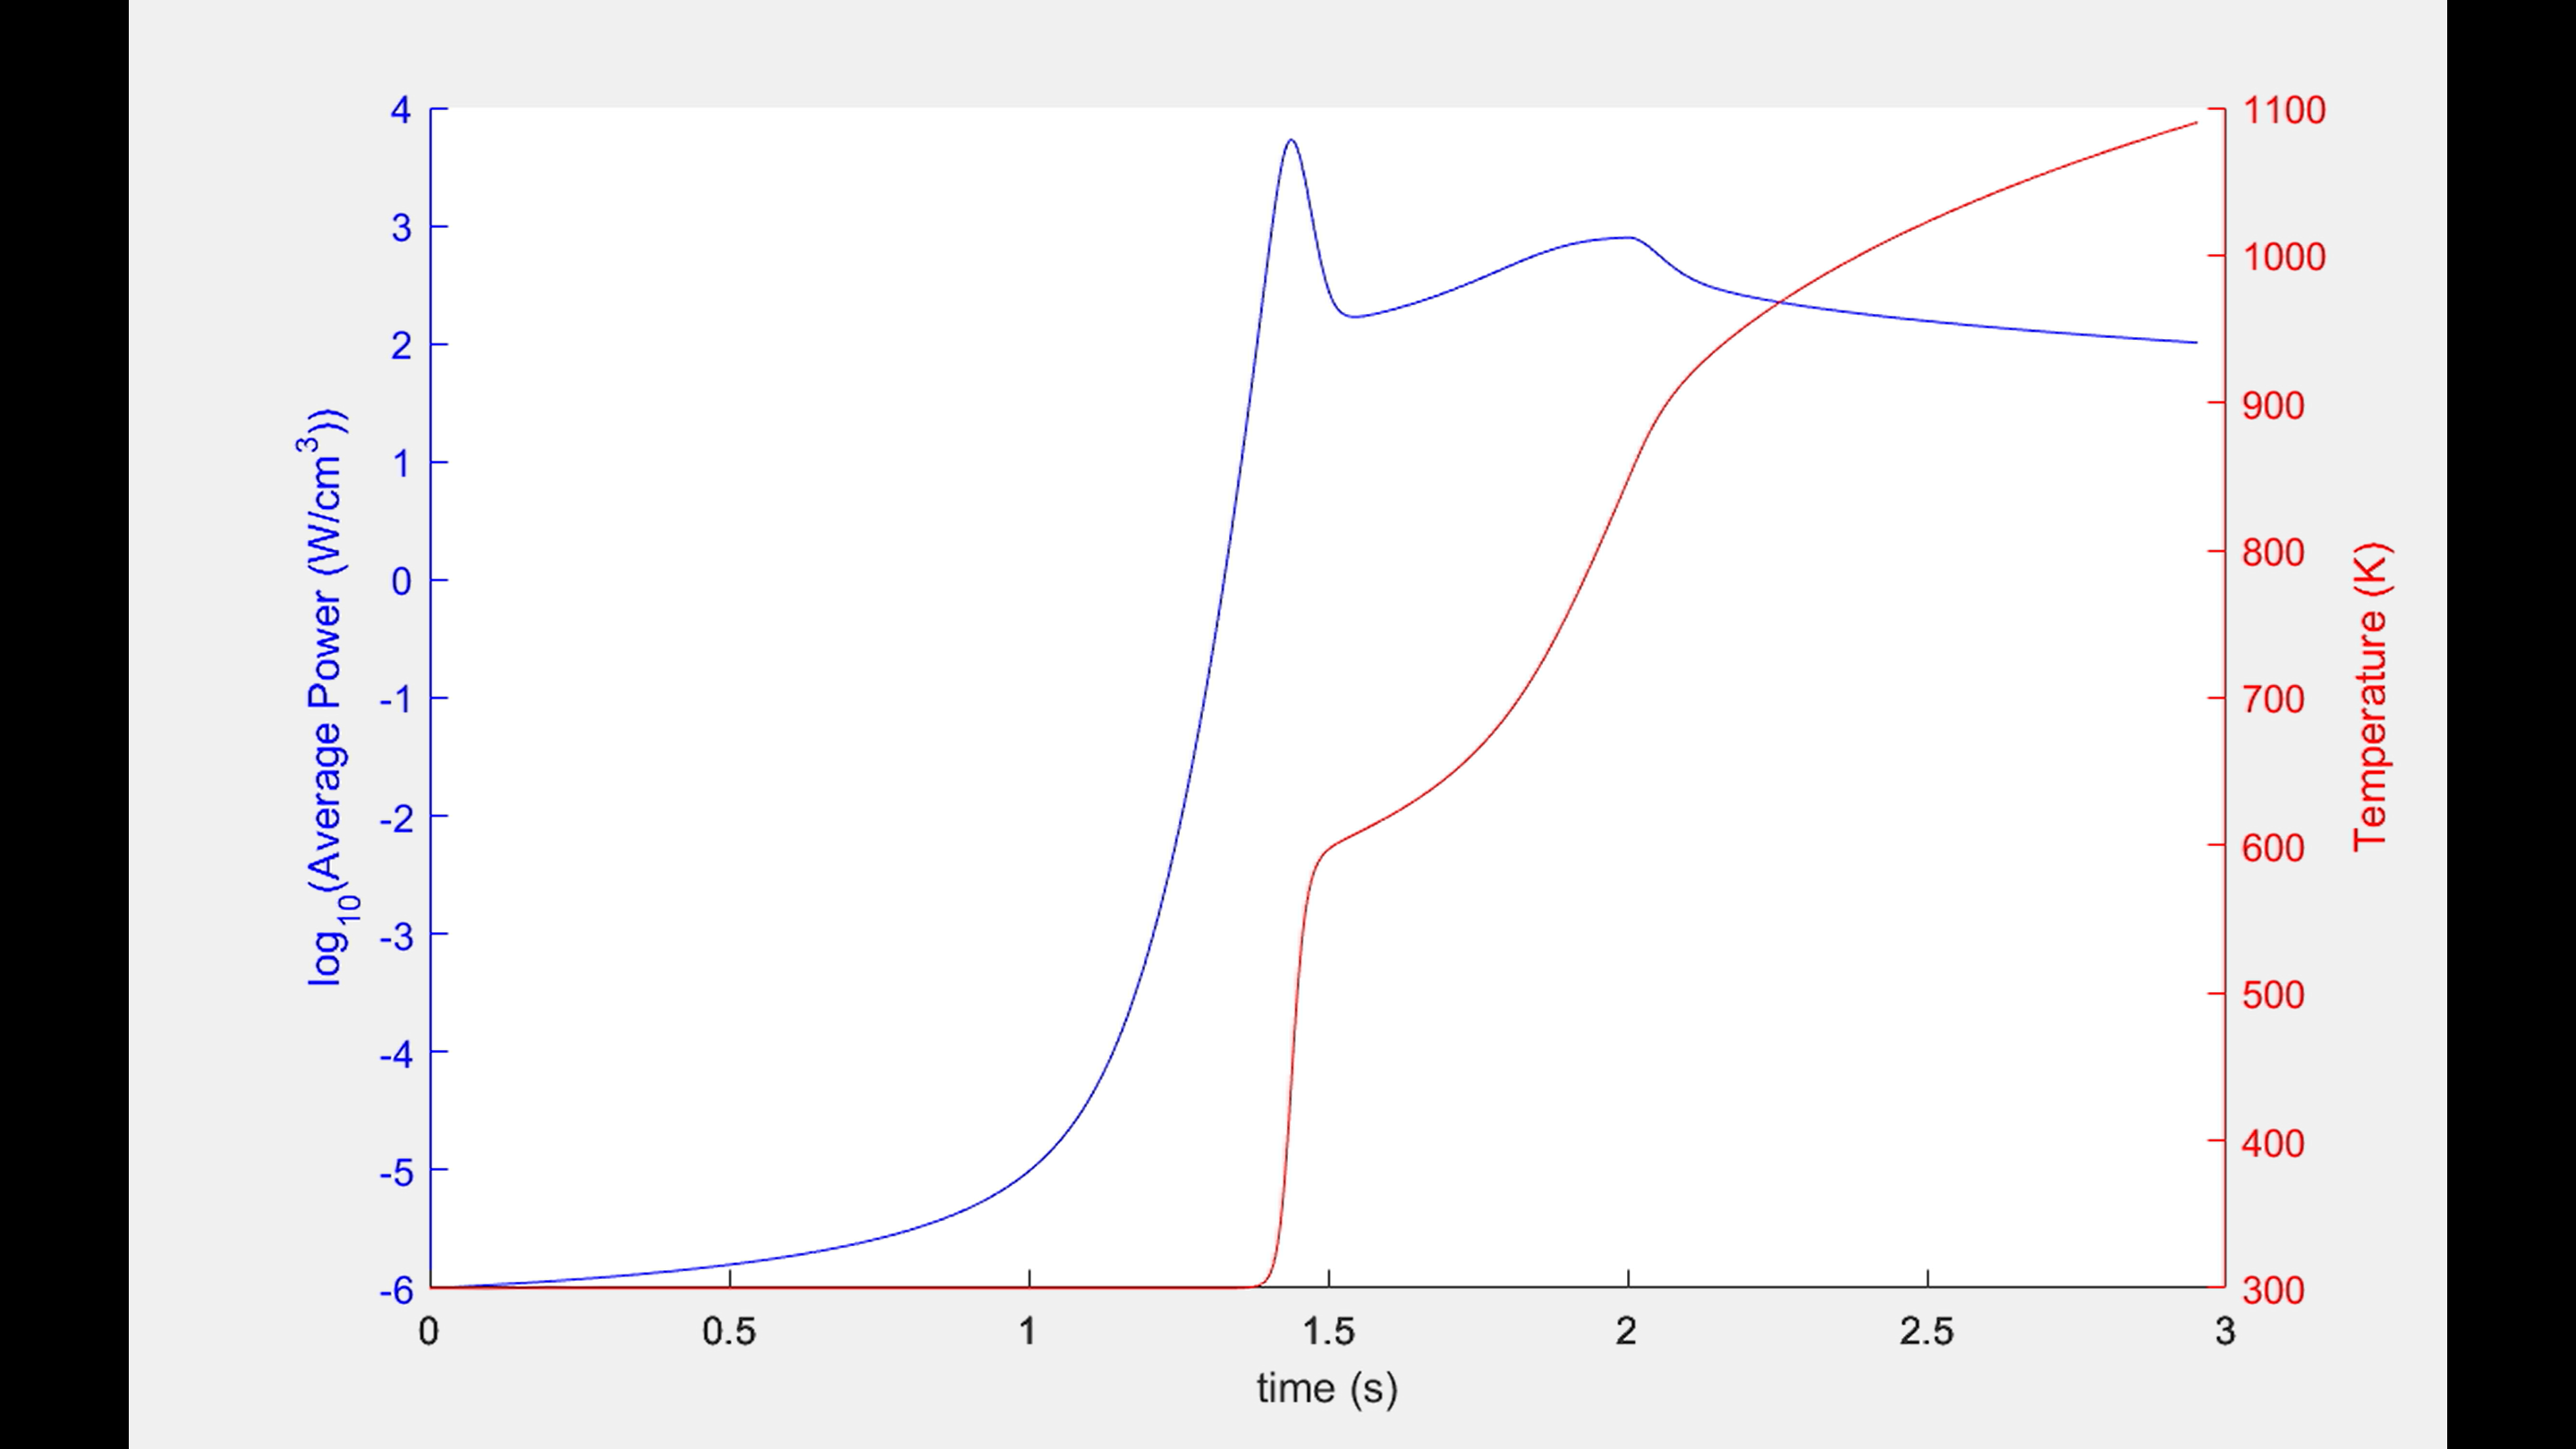
\includegraphics[width=\linewidth]{\FiguresDir/lra_profile.png}
\caption{LRA baseline temperature and power profile}
\label{fig:lra_profile}
\end{figure}

\begin{figure}[htbp!]
\centering
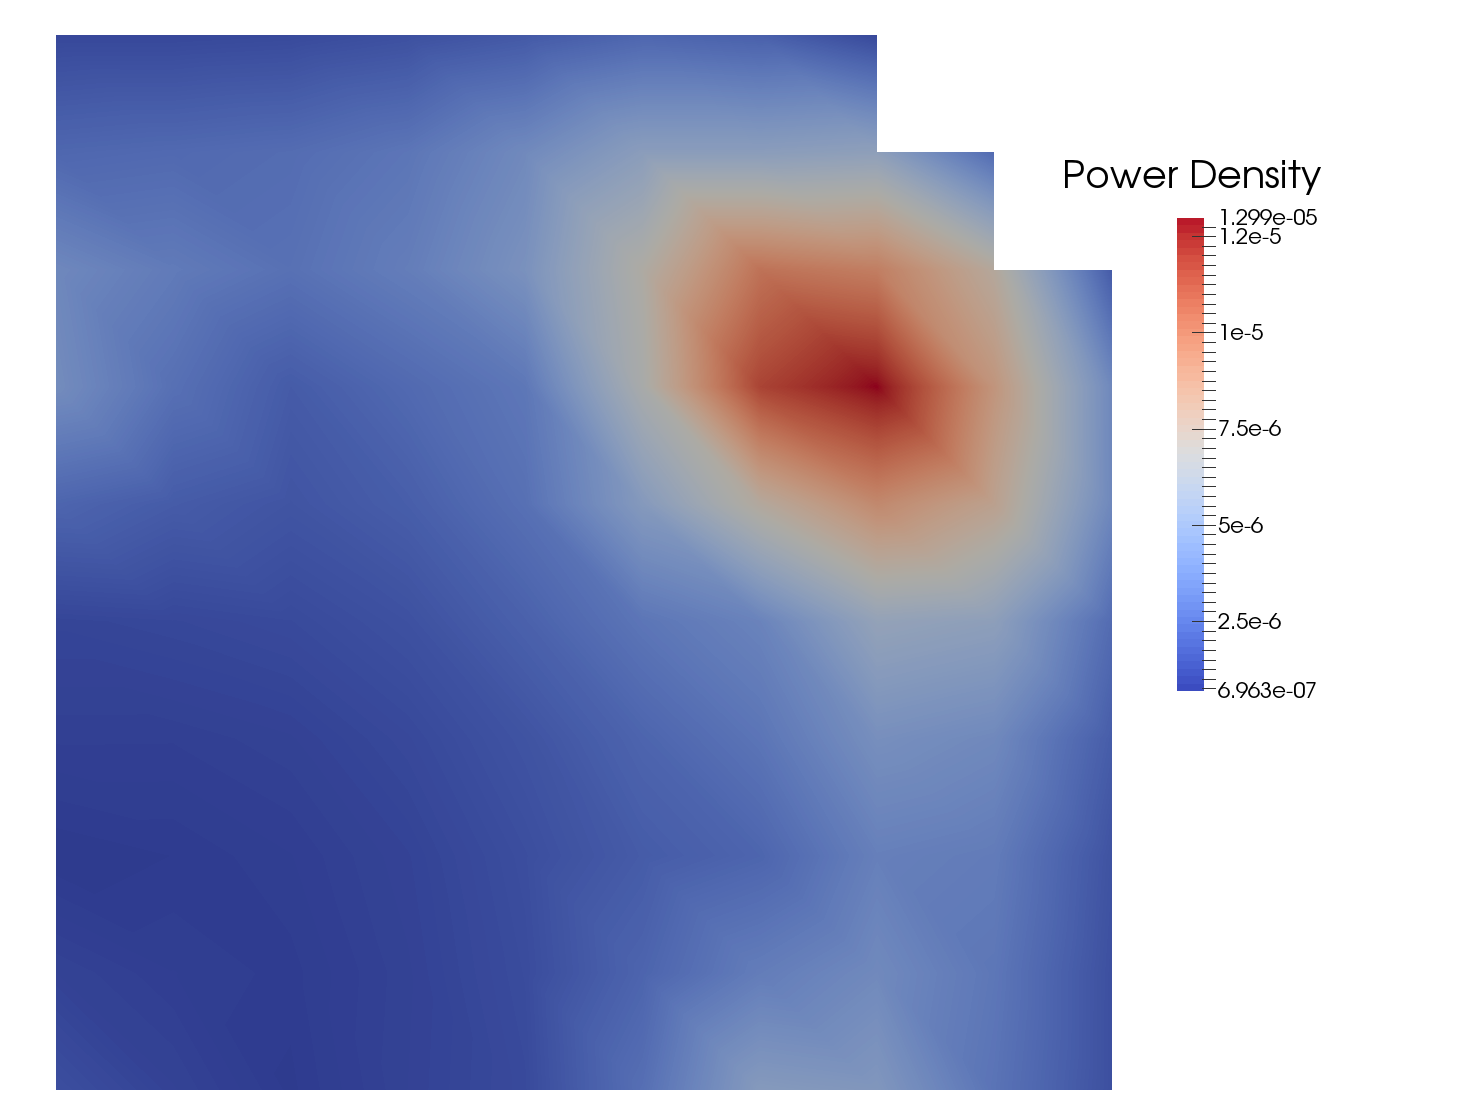
\includegraphics[width=\linewidth]{\FiguresDir/lra_profile2D.png}
\caption{LRA baseline spacial power profile at $t=1.44 s$}
\label{fig:lra_profile2D}
\end{figure}

\begin{table}[!htbp]
\begin{center}
%\resizebox{\linewidth}{!}{
\begin{tabular}{|l|cc|}
\hline
Calculation  &  Baseline & Sutton (Spandex 1936) \\
\hline
No. of Spatial Nodes	& 3872 		& 1936 \\
Eigenvalue 				& 0.99637	& 0.99637 \\
No. of Time Steps 		& 6000 		& 23,890 \\
Time to Peak Power (s) 	& 1.441 	& 1.441 \\
Peak Power (W/cm$^3$) 	& 5456 		& 5461 \\
\hline
\end{tabular}
%}
\end{center}
\caption{LRA baseline verification}
\label{tab:base}
\end{table}

\begin{figure}[!htbp]
\centering
\begin{subfigure}[!htbp]{0.49\textwidth}
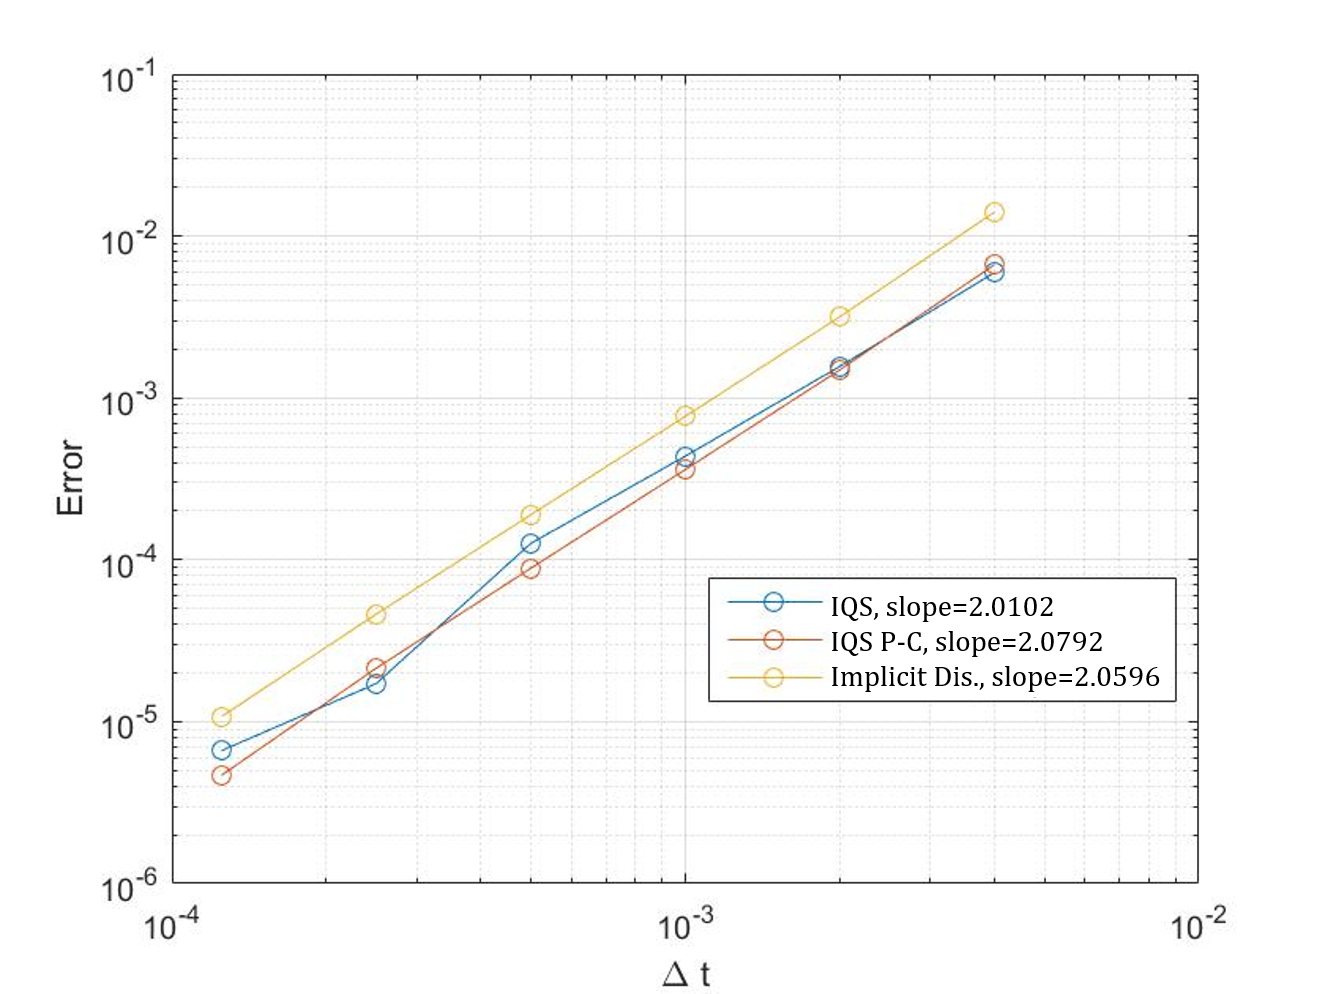
\includegraphics[width=\textwidth]{\FiguresDir/lra_bad.png}
\caption{Only one temperature update per macro step}
\label{fig:lra_bad}
\end{subfigure}
\begin{subfigure}[!htbp]{0.49\textwidth}
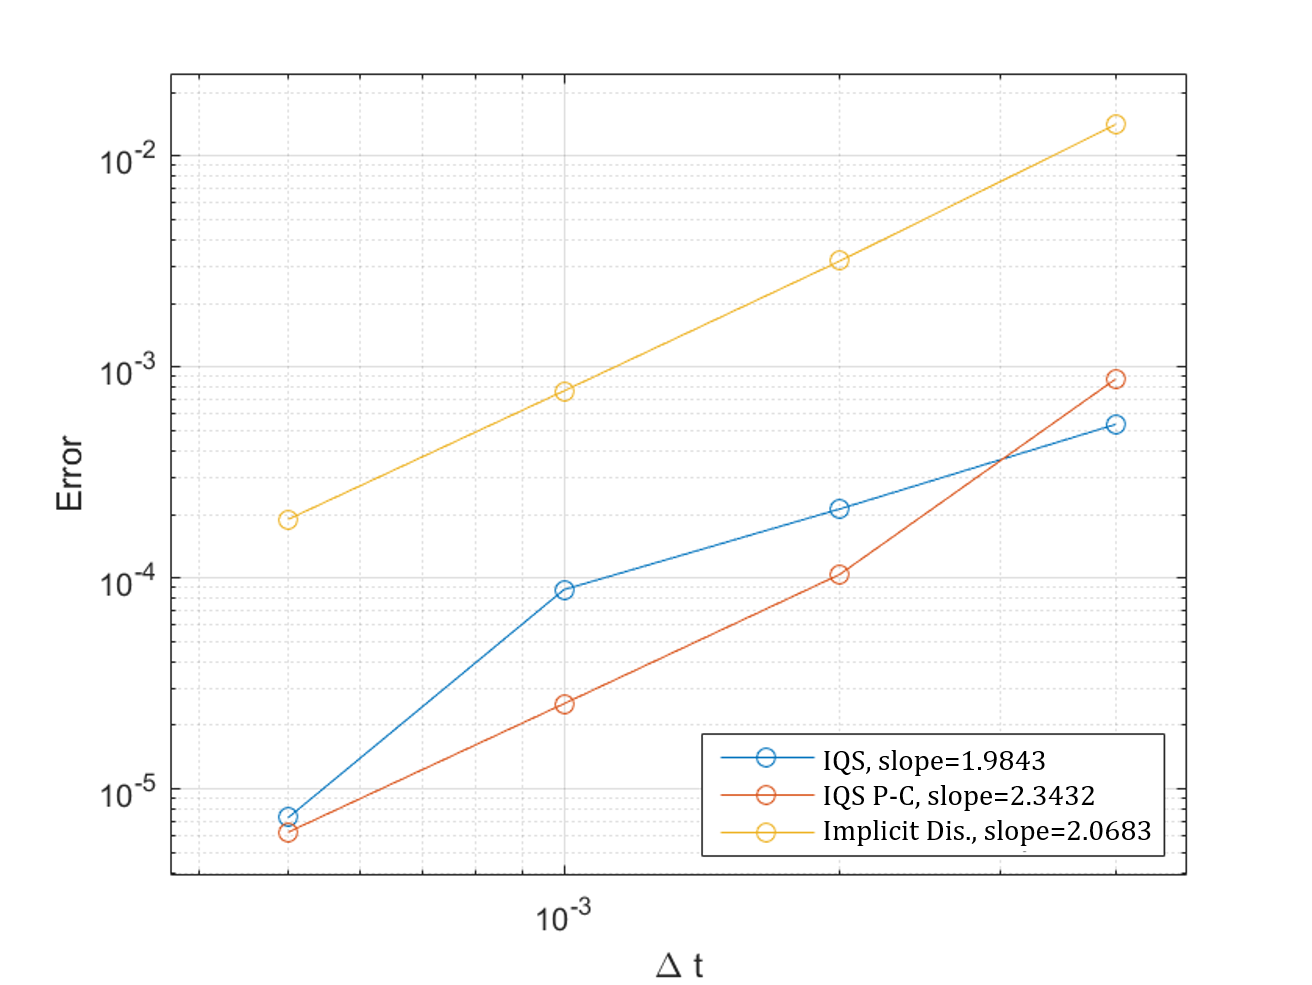
\includegraphics[width=\textwidth]{\FiguresDir/lra_mp_convergence.png}
\caption{Five temperature updates per macro step}
\label{fig:lra_mpconv}
\end{subfigure}
\caption{LRA error convergence plots}
\end{figure}

\begin{figure}[htbp!]
\centering
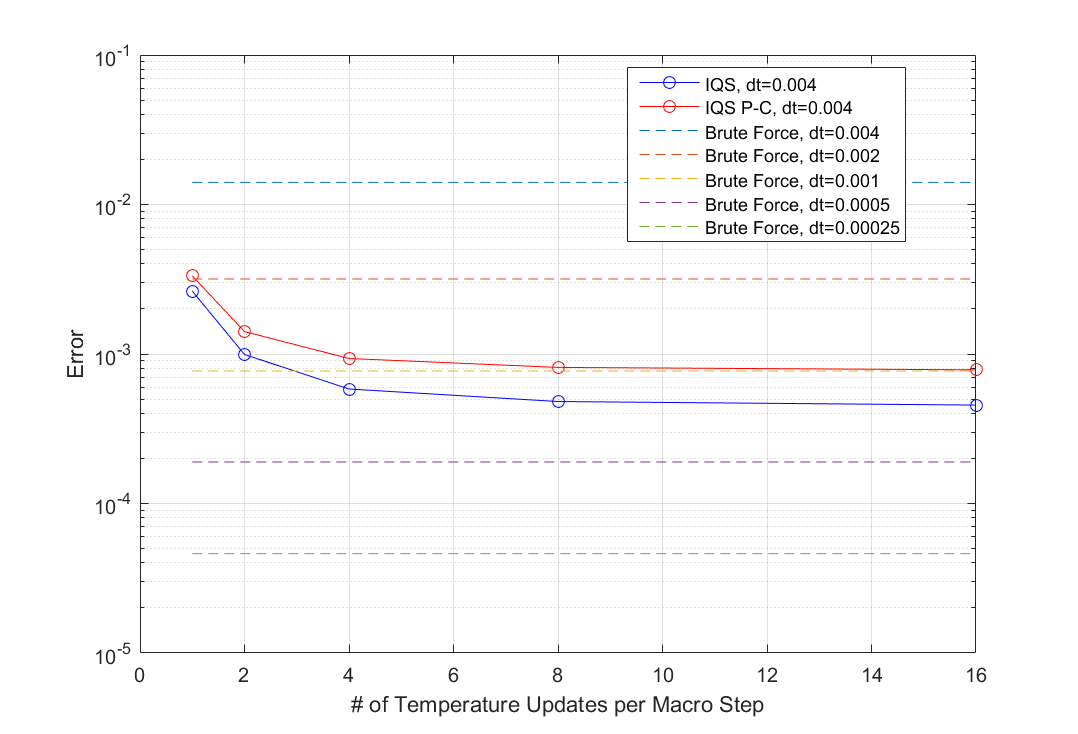
\includegraphics[width=\linewidth]{\FiguresDir/lra_mp.png}
\caption{Error plot with various temperature updates per macro step}
\label{fig:mp}
\end{figure}

The convergence plots show that updating temperature and the PRKE parameters within a macro step has a significant effect on the performance of IQS.  With only one update, IQS was only slightly better than implicit discretization, implicit discretization required about 150\% more time steps than IQS for the same error.  While 5 temperature updates showed a much more significant IQS performance, implicit discretization required about 400\% more time steps than IQS for the same error.  \fig{fig:mp} shows that error has a convergent behavior for the number of temperature updates.  This convergence makes sense because temperature can only be so accurate before the error in shape is dominating. Table \ref{tab:ndiff_lra} shows the run time results for the implicit discretization calculations. The number of GMRES linear iterations is included because it is proportional measure of the computational effort. Tables \ref{tab:iqs_lra} and \ref{tab:iqspc_lra} present the IQS run-times with various numbers of temperature updates.  These run-times are based on total alive time of the execution where the diffusion evaluation is distributed over 24 processors. These run-times show a marginal performance for IQS and impressive performance for IQS P-C.  Some of the execution times were able to decrease from implicit discretization with the same number of macro steps because IQS is better equipped to resolve the nonlinearity between temperature and amplitude. Furthermore, there does seem to be an ideal number of temperature updates to optimize execution time: IQS only needs one and IQS P-C seems to be ideal at 4 updates. This discrepancy in the number of updates shows that a adaptive type implementation of the updates would be ideal, and could enforce a constant error over the transient. It is also important to compare the error of implicit discretization with IQS at one update and IQS P-C at 4 updates.  IQS shows an error comparable to implicit discretization at $\Delta t = 0.002$, signifying an actual increase in runtime by -34.1\%.  IQS P-C shows an error less than implicit discretization at $\Delta t = 0.002$, signifying an actual increase in runtime by <-34.9\%.

\begin{table}[!htbp]
\begin{center}
%\resizebox{\linewidth}{!}{
\begin{tabular}{|l|l|ccc|}
\hline
Run  &  $\Delta t$ & Error & Runtime (hr) & Linear Iter.\\
\hline
1	& 4.0e-3	& 1.407e-2 	& 4.11	& 7.13e4	\\
2	& 2.0e-3	& 3.174e-3 	& 6.01	& 9.49e4 	\\
3 	& 1.0e-3 	& 7.690e-4 	& 10.38	& 1.45e5	\\
4 	& 5.0e-4 	& 1.892e-4 	& 21.91	& 2.08e5	\\
5 	& 2.5e-4	& 4.590e-5 	& 25.23	& 3.16e5	\\
\hline
\end{tabular}
%}
\end{center}
\caption{Implicit discretization run time results}
\label{tab:ndiff_lra}
\end{table}

\begin{table}[!htbp]
\begin{center}
%\resizebox{\linewidth}{!}{
\begin{tabular}{|l|l|ccc|}
\hline
	&  Temperature 	&  		& Runtime 	& \% Increase	\\
Run	&  Updates 	& Error & (hr)		& in Runtime$^*$\\
\hline
1	& 1		& 2.612e-3 	& 3.96 	& -3.18\%	\\
2	& 2		& 9.893e-4 	& 6.02	&  47.1\%	\\
3 	& 4 	& 5.796e-4 	& 7.87	&  92.3\%	\\
4 	& 8 	& 4.772e-4 	& 12.61	& 207.9\% 	\\
5 	& 16	& 4.516e-4 	& 22.14	& 440.7\%	\\
\hline
\end{tabular}
%}
\\
$^*$ difference in runtime from $\Delta t = 0.004$ implicit discretization 
\caption{IQS run time results with $\Delta t = 0.004$}
\label{tab:iqs_lra}
\end{center}
\end{table}

\begin{table}[!htbp]
\begin{center}
%\resizebox{\linewidth}{!}{
\begin{tabular}{|l|l|ccc|}
\hline
	&  Temperature 	&  		& Runtime 	& \% Increase	\\
Run	&  Updates 	& Error & (hr)		& in Runtime$^*$\\
\hline
1	& 1		& 3.488e-3 	& 2.91 	& -28.9\%	\\
2	& 2		& 1.349e-3 	& 3.73	& -9.00\%	\\
3 	& 4 	& 9.161e-4 	& 3.97	& -3.04\%	\\
4 	& 8 	& 8.052e-4 	& 5.39	&  31.7\%	\\
5 	& 16	& 7.905e-4 	& 8.19	&  100\%	\\
\hline
\end{tabular}
%}
\\
$^*$ difference in runtime from $\Delta t = 0.004$ implicit discretization 
\caption{IQS PC run time results with $\Delta t = 0.004$}
\label{tab:iqspc_lra}
\end{center}
\end{table}

The performance of the quasi-statics can also be explained by the computation of the dynamical time scale described by \sct{sect:tau}.  \fig{fig:LRAtc} shows the time scale profile over the transient, computed using \eqt{eq:tau2}.  This plot shows that in a implicit discretization simulation, the flux dominates the time dependent behavior, while temperature lags in its variance for the majority of the transient.  In an IQS simulation, the time scale behavior of amplitude almost exactly matches the flux, while shape is more varying than temperature throughout most of the transient.  The large $\tau$ for temperature during the beginning of the transient shows that adaptation of the number of updates is important; computational expense on temperature evaluations is being wasted during this time.

\begin{figure}[htbp!]
\centering
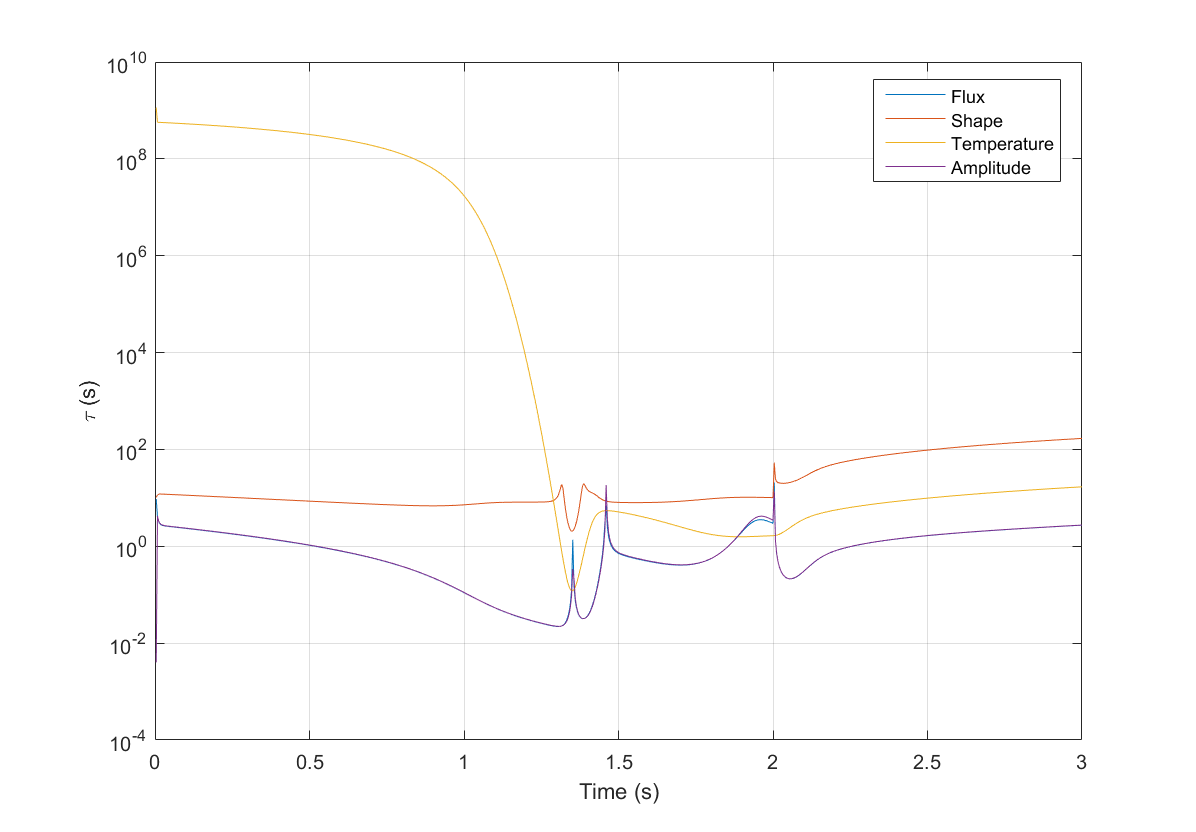
\includegraphics[width=\linewidth]{\FiguresDir/time_constant_lra.png}
\caption{Dynamical time scale for LRA benchmark}
\label{fig:LRAtc}
\end{figure}

\subsection{LRA with Time Adaptation}

\fig{fig:lra_dt2} shows the power profile of the LRA with time adaptation of implicit discretization and IQS P-C, and \tbl{tab:lra_dt2} compiles the results. These time adaptation results show the significant decrease in macro time steps required for IQS P-C. These profiles were obtaining with only one temperature update per macro step; so based on previous results, the IQS P-C performance would improve even more with more updates.

\begin{figure}[!htbp]
\centering
\begin{subfigure}[!htbp]{0.49\textwidth}
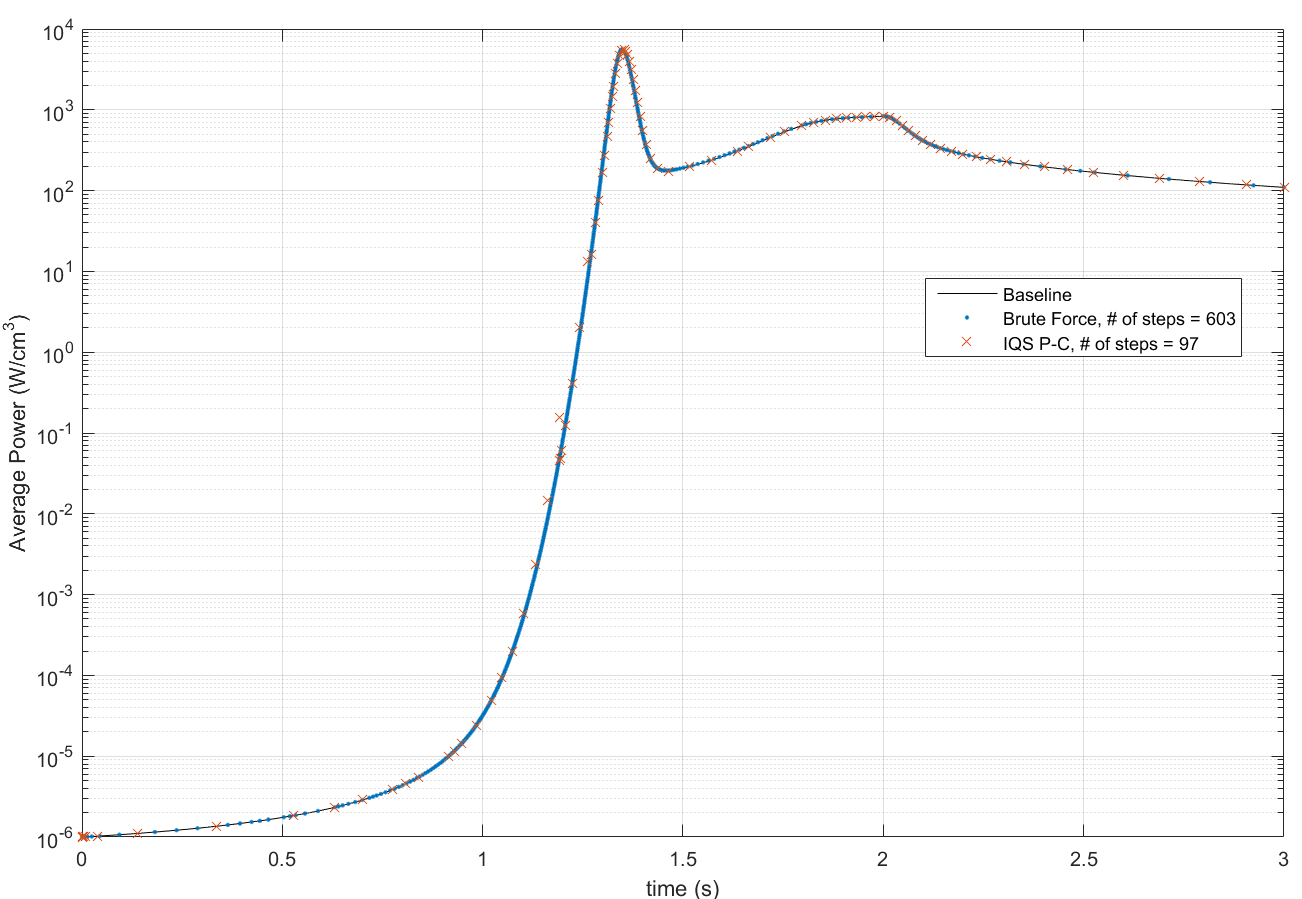
\includegraphics[width=\textwidth]{\FiguresDir/LRA_DT2.png}
\caption{Full power profile}
\end{subfigure}
\begin{subfigure}[!htbp]{0.49\textwidth}
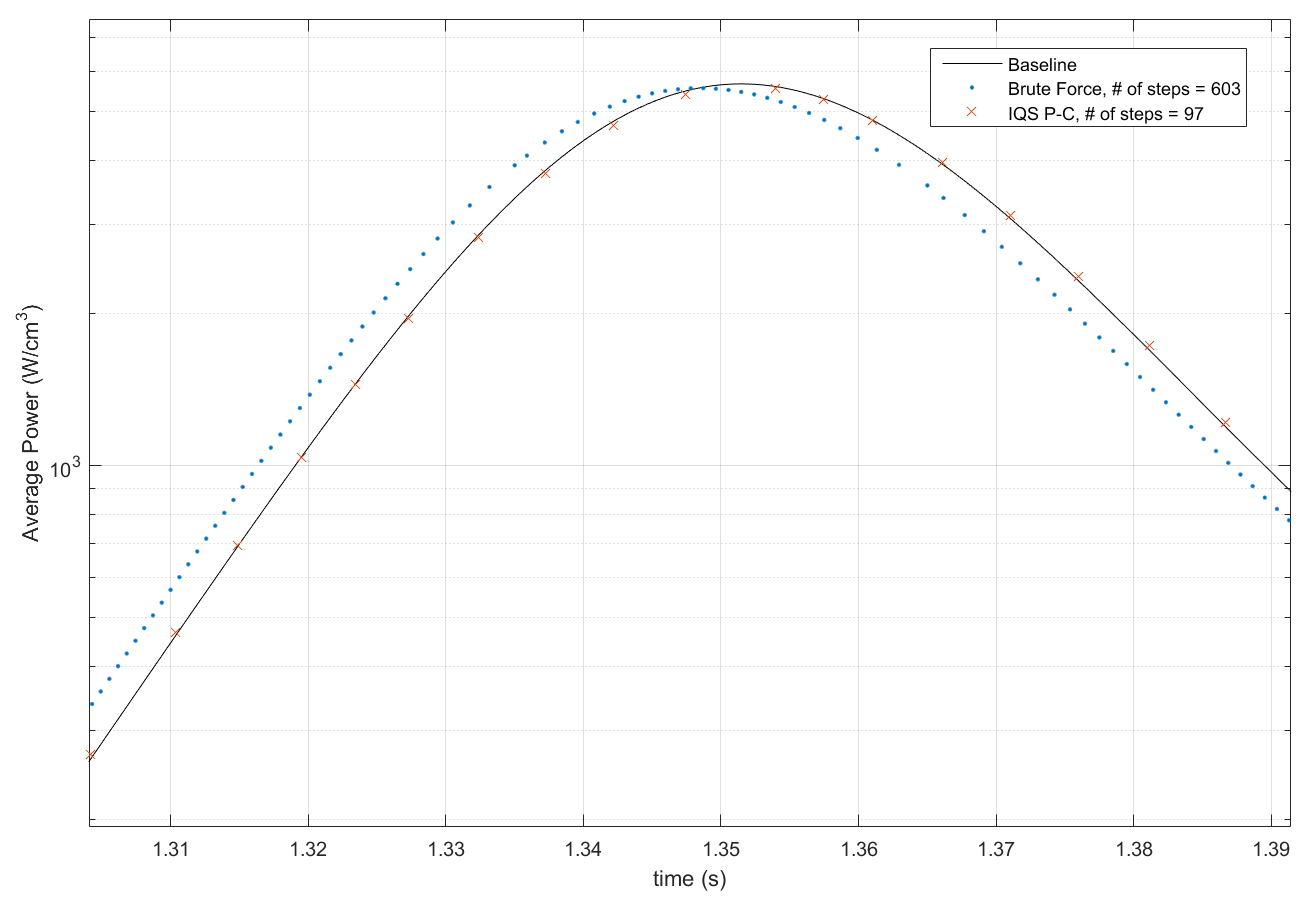
\includegraphics[width=\textwidth]{\FiguresDir/LRA_DT2_peak.png}
\caption{Peak power profile at peak}
\end{subfigure}
\caption{LRA power profile with time adaptation of implicit discretization and IQS P-C}
\label{fig:lra_dt2}
\end{figure}

\begin{table}
\begin{center}
\resizebox{\textwidth}{!}{
\begin{tabular}{|l|l|l|l|l|l|l|}
\hline
 & \multicolumn{3}{|c|}{Implicit Dis.} & \multicolumn{3}{|c|}{IQS P-C} \\
\hline
Event & Power (W/cm$^3$) & Error & Steps & Power (W/cm$^3$) & Error & Steps \\
\hline
Max Power & 5567.3 & 0.019454 & 423 & 5568.3 & 0.019274 & 47 \\
End (3 s) & 109.66 & 2.3650e-4 & 603 & 109.65 & 3.0622e-4 & 97 \\
\hline
\end{tabular}}
\end{center}
\caption{LRA step doubling adaptation results with implicit discretization and IQS P-C}
\label{tab:lra_dt2}
\end{table}


\section{TREAT Transient-15 Problem}

Transient 15 is a test case based on the TREAT core. The preliminary purpose of this model was to match an early test of TREAT; due to lack of experimental data and procedures, model validation was impossible \cite{mammoth}. Therefore, ultimate purpose of this simulation in Rattlesnake is to test the model's fidelity with the thermal feedback of TREAT, but it is not meant to exactly match any previous experiments.  Nevertheless, the goal of the following simulations is to test IQS and its time scale based treatment of temperature with a more complex model. The model involves a 159-element "small core" configuration of TREAT, shown in \fig{fig:Tran15_config} \cite{Tran15}. \fig{fig:Tran15_mesh} shows the meshing techniques of the model \cite{mammoth}. To ease computation, the fully homogenized version (without air gaps) was used  for the following simulations. Transient 15 involves an 11-energy group diffusion approximation and is discretized into $355,712$ hexahedral continuous finite elements totaling $4,109,523$ degrees of freedom.  The three-second transient involves a linear ramp decrease in the absorption cross section throughout the control rod region. \fig{fig:Tran15} shows a visualization of the flux profile within the core, hidden is the massive amount of graphite surrounding the core.   

\begin{figure}[htbp!]
\centering
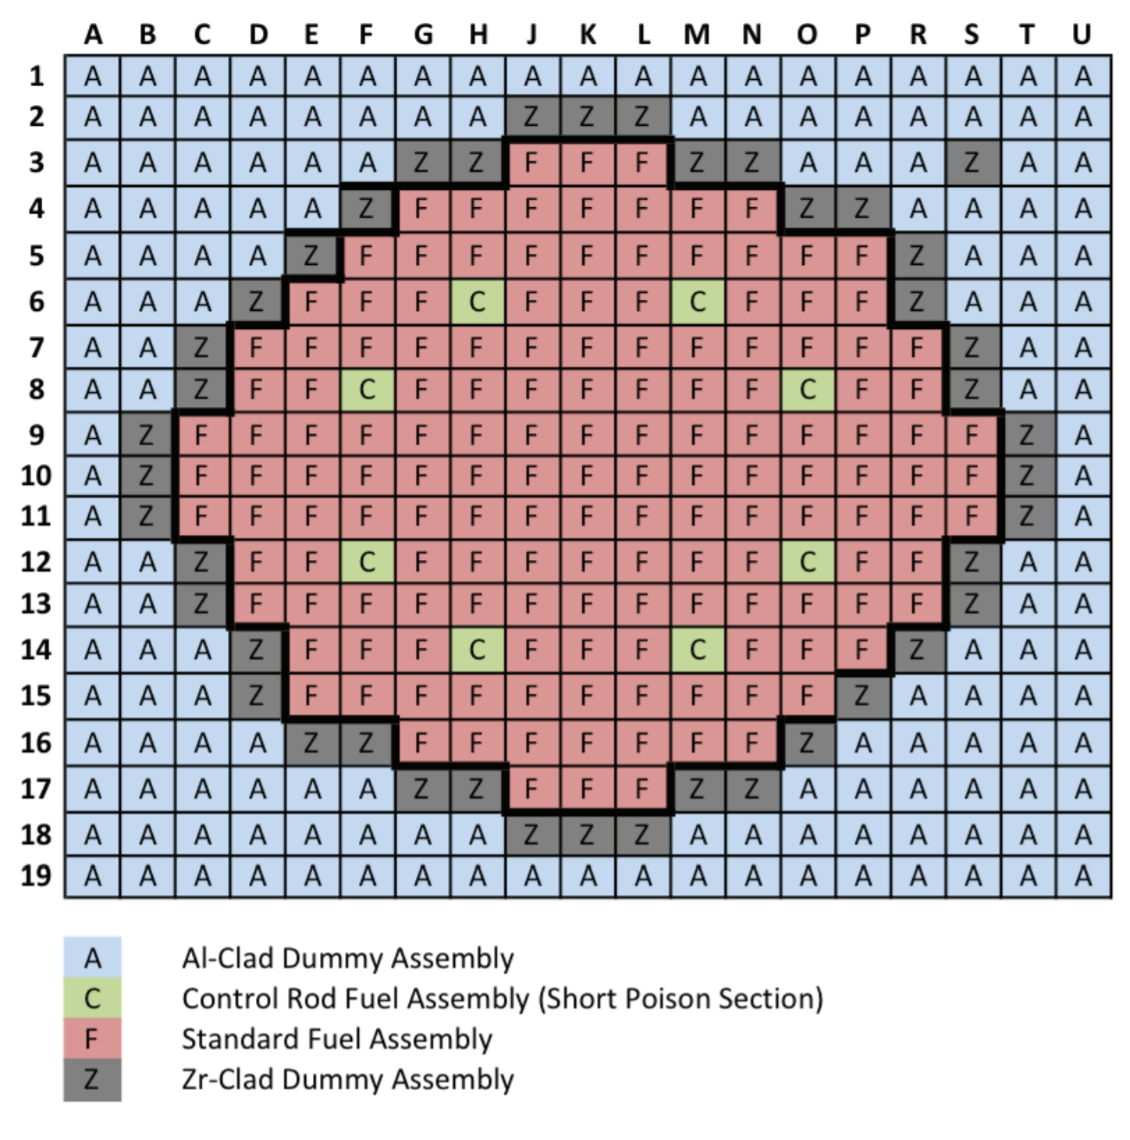
\includegraphics[width=0.7\linewidth]{\FiguresDir/Tran15_config.png}
\caption{Transient 15 159-element small core configuration}
\label{fig:Tran15_config}
\end{figure}

\begin{figure}[!htbp]
\centering
\begin{subfigure}[!htbp]{0.49\textwidth}
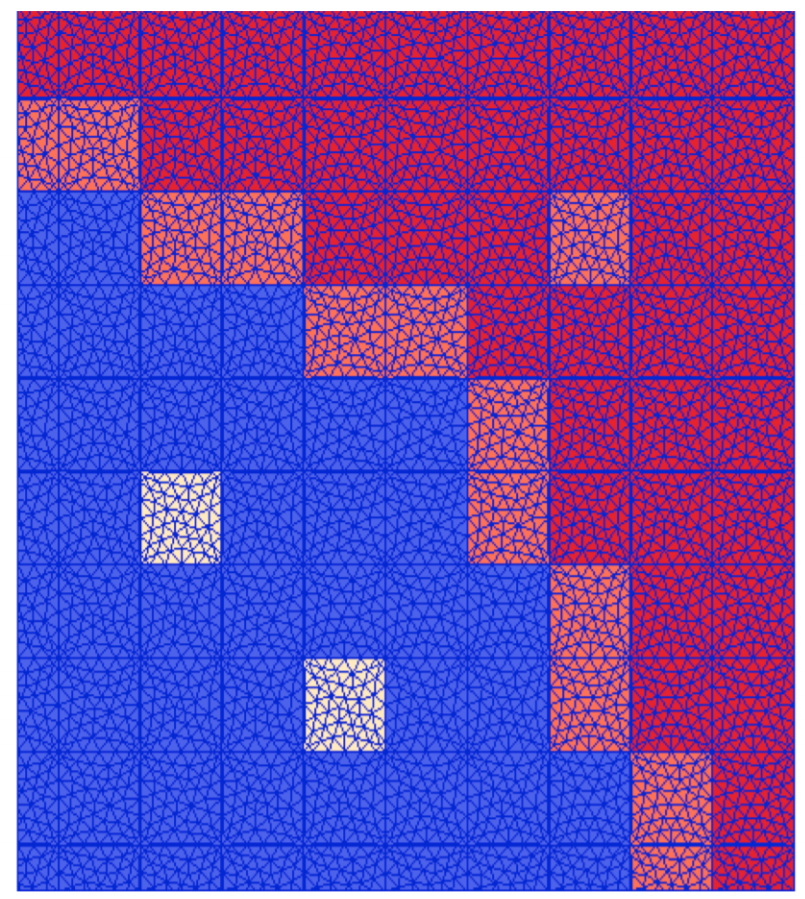
\includegraphics[width=\textwidth]{\FiguresDir/Tran15_mesh_fine.png}
\caption{Explicit meshing of air channels}
\label{fig:Tran15_mesh_fine}
\end{subfigure}
\begin{subfigure}[!htbp]{0.49\textwidth}
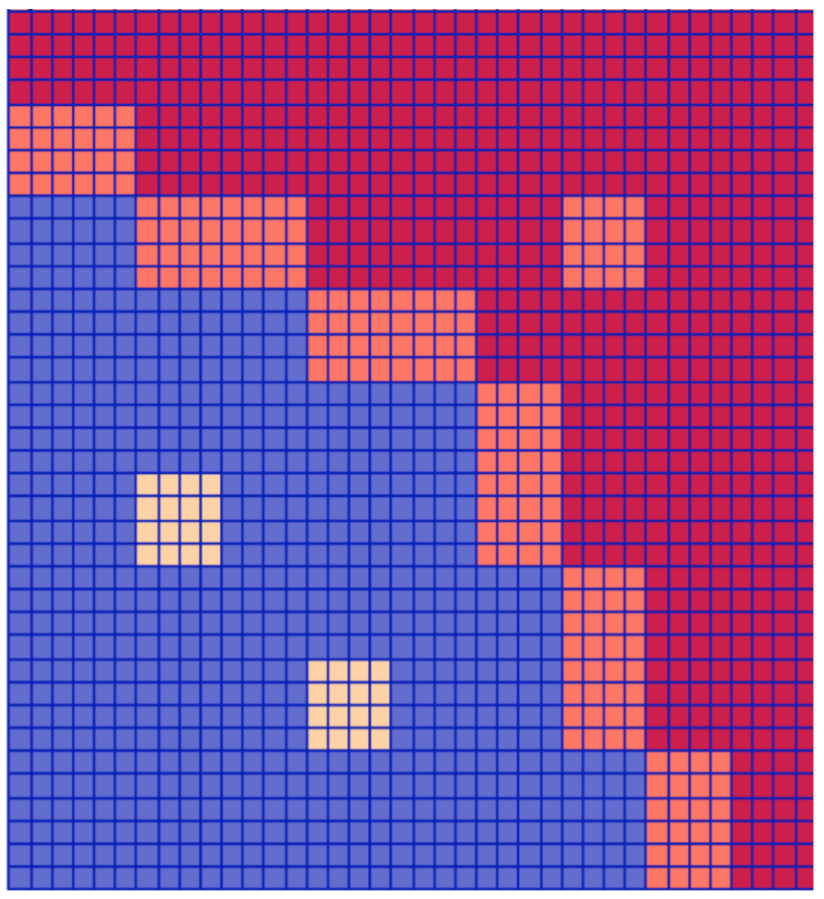
\includegraphics[width=\textwidth]{\FiguresDir/Tran15_mesh_homo.png}
\caption{Fully homogenized fuel elements}
\label{fig:Tran15_mesh_homo}
\end{subfigure}
\caption{Top quarter view of Transient 15 mesh}
\label{fig:Tran15_mesh}
\end{figure}

\begin{figure}[htbp!]
\centering
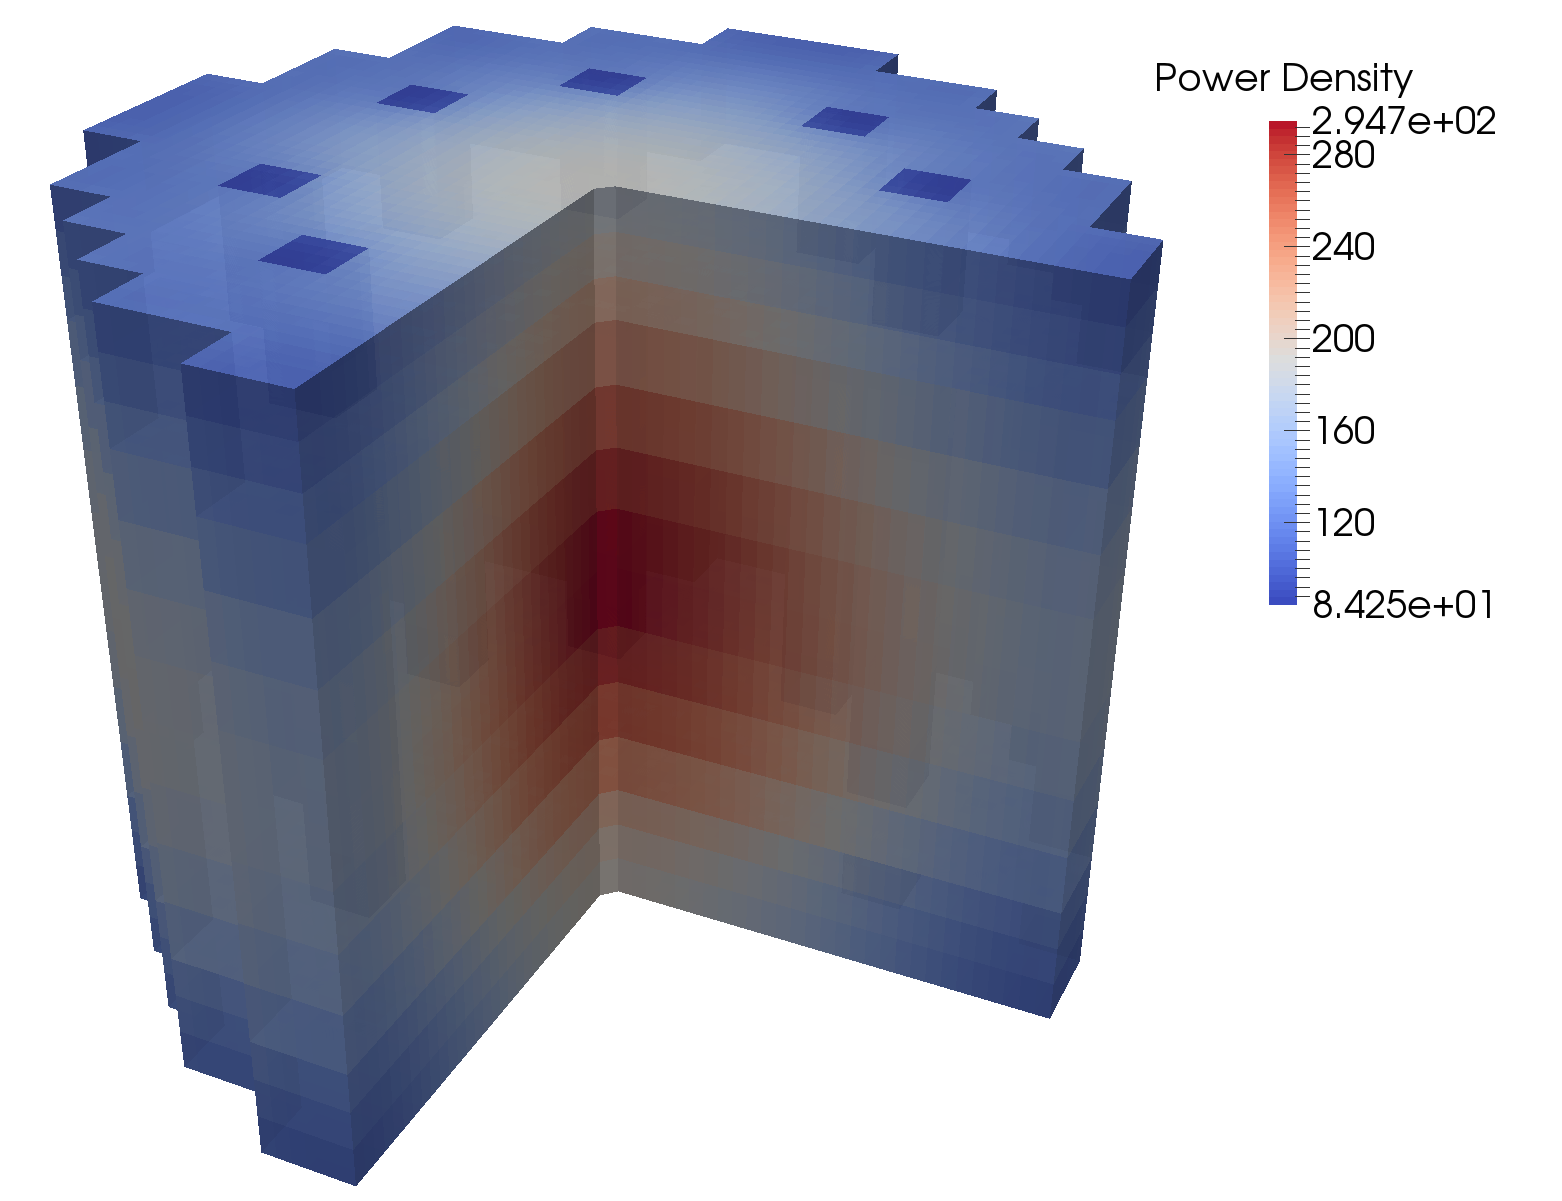
\includegraphics[width=0.6\linewidth]{\FiguresDir/Tran15_core2.png}
\caption{Transient 15 core power profile at peak power}
\label{fig:Tran15}
\end{figure}

\subsection{Transient-15 Temperature Feedback}

The Transient-15 model uses a adiabatic temperature feedback mechanism, similar to the one explored by the LRA. \eqt{eq:temp2} describes the heat up of the fuel.  It is very similar, except the specific heat is now dependent on temperature is described by \eqt{eq:cp}.  The temperature evaluation is identical to the one described in LRA section, except a Newton iteration process is employed to resolve the nonlinearity from the specific heat term.  The feedback to the cross-sections are applied using linear interpolation of tabular data provided by INL.

\be
\rho c_p(T) \frac{\partial T(\vec{r},t)}{\partial t} = \kappa_f \sum^G_{g=1}\Sigma_f^g \phi^g(\vec{r},t)
\label{eq:temp2}
\ee

\be
c_p = -5.8219\text{e-}10T^3 - 4.3694\text{e-}7T^2 + 2.8369\text{e-}3T -1.009\text{e-}2 \ (J/g/K)
\label{eq:cp}
\ee

\subsection{Transient-15 Multiphysics Time Scale Results}

In order to test the temperature feedback treatment, six different scenarios were run: a baseline with a very small time step, implicit discretization, IQS with one and 5 temperature updates per macro step, and IQS P-C with one and 5 updates.  \fig{fig:Tran15_profile} shows the baseline power and temperature profile for the Transient-15 example.  \tbl{tab:tran15} shows the error and runtime results.

\begin{figure}[htbp!]
\centering
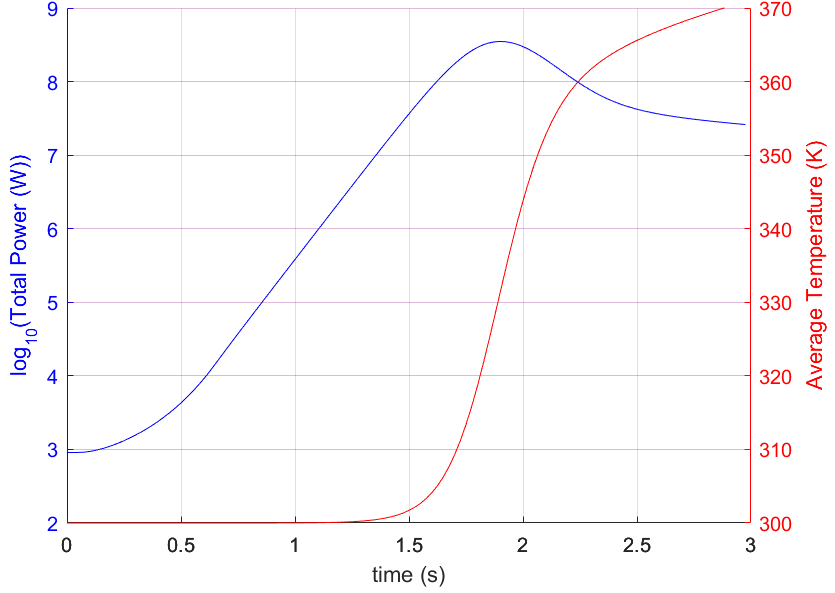
\includegraphics[width=\linewidth]{\FiguresDir/Tran15_profile.png}
\caption{Transient 15 total power and average temperature profile during transient}
\label{fig:Tran15_profile}
\end{figure}

\begin{table}[htb]
\begin{center}
\resizebox{\linewidth}{!}{
\begin{tabular}{|l|ccccccc|}
\hline
 & No.	& Max &	Time at Max &	Max Average &	\% Increase &	Max Power & Linear	\\
Method & of Steps &	Power (W) &	Power (s) &	Temperature (K) & Runtime$^*$ & Error & Iterations \\
\hline
Baseline 			& 3000 	& 3.5039e+08 & 1.901 & 371 &	---		&	---		 & ---		\\
Implicit Dis. 		& 300 	& 3.5011e+08 & 1.90  & 371 &	---		&	7.875e-4 & 41020	\\
IQS 				& 300	& 3.5036e+08 & 1.90  & 371 & -11.9\%	&	8.385e-5 & 23949	\\
IQS (5 updates) 	& 300 	& 3.5040e+08 & 1.90  & 371 &  49.7\%	&	3.687e-5 & 24035	\\
IQS P-C 			& 300 	& 3.5065e+08 & 1.90  & 371 &  -2.1\%	&	7.527e-4 & 39020	\\
IQS P-C (5 updates) & 300 	& 3.5043e+08 & 1.90  & 371 &  26.5\%	&	1.227e-4 & 37866	\\
\hline
\end{tabular}
}
\end{center}
\vspace{-3mm}
$^*$ difference in runtime from implicit discretization 
\caption{Transient-15 Error and Runtime Results}
\label{tab:tran15}
\end{table}

The results from \tbl{tab:tran15} show similar performance of IQS with the temperature updates as the LRA. Again, the number of linear GMRES iterations is shown as a measure of computational expense. However, these iterations do not consider the temperature updates, so the iterations of the simulations with multiple updates should be taken with a grain of salt. IQS with 1 temperature update shows a performance that reduces the error to approximately a tenth of the implicit discretization error, and reduces the execution time by about 12\%.  This shows that IQS was able to resolve the nonlinearity between flux and temperature with significantly fewer diffusion evaluations.  Having IQS with 5 updates significantly increased the execution time for the same time step, but the error was reduced.  Comparing this error to a similar implicit discretization error at a smaller time step could show that the runtime was reduced. IQS P-C performed not nearly as well as it did with the LRA benchmark, but still proved to be effective.  Having 5 updates for IQS P-C increased the runtime marginally, but decreased the error significantly.  The transient profile of the variables' dynamical time scales is shown in \fig{fig:tran15tc}.  This plot exhibits a similar response to that of the LRA. The response of temperature shows that the updates are a computational frugal treatment of the feedback and adaptation of the number of updates is vital for optimization. \\

\begin{figure}[htbp!]
\centering
\includegraphics[width=0.7\linewidth]{\FiguresDir/time_constant_tran15.png}
\caption{Dynamical time scale for the Transient 15 example}
\label{fig:tran15tc}
\end{figure}

\subsection{Transient-15 with Time Adaptation}

\fig{fig:Tran15_dt2} shows the power profile of the LRA with time adaptation of implicit discretization and IQS P-C.  These plots show that IQS P-C requires marginally fewer macro time steps than implicit discretization, but is qualitatively much closer to the baseline profile. Like the LRA step doubling results, IQS P-C only performs one temperature update per macro step. Adding more updates would most likely improve the error, but increase the computation time significantly. 

\begin{figure}[!htbp]
\centering
\begin{subfigure}[!htbp]{0.49\textwidth}
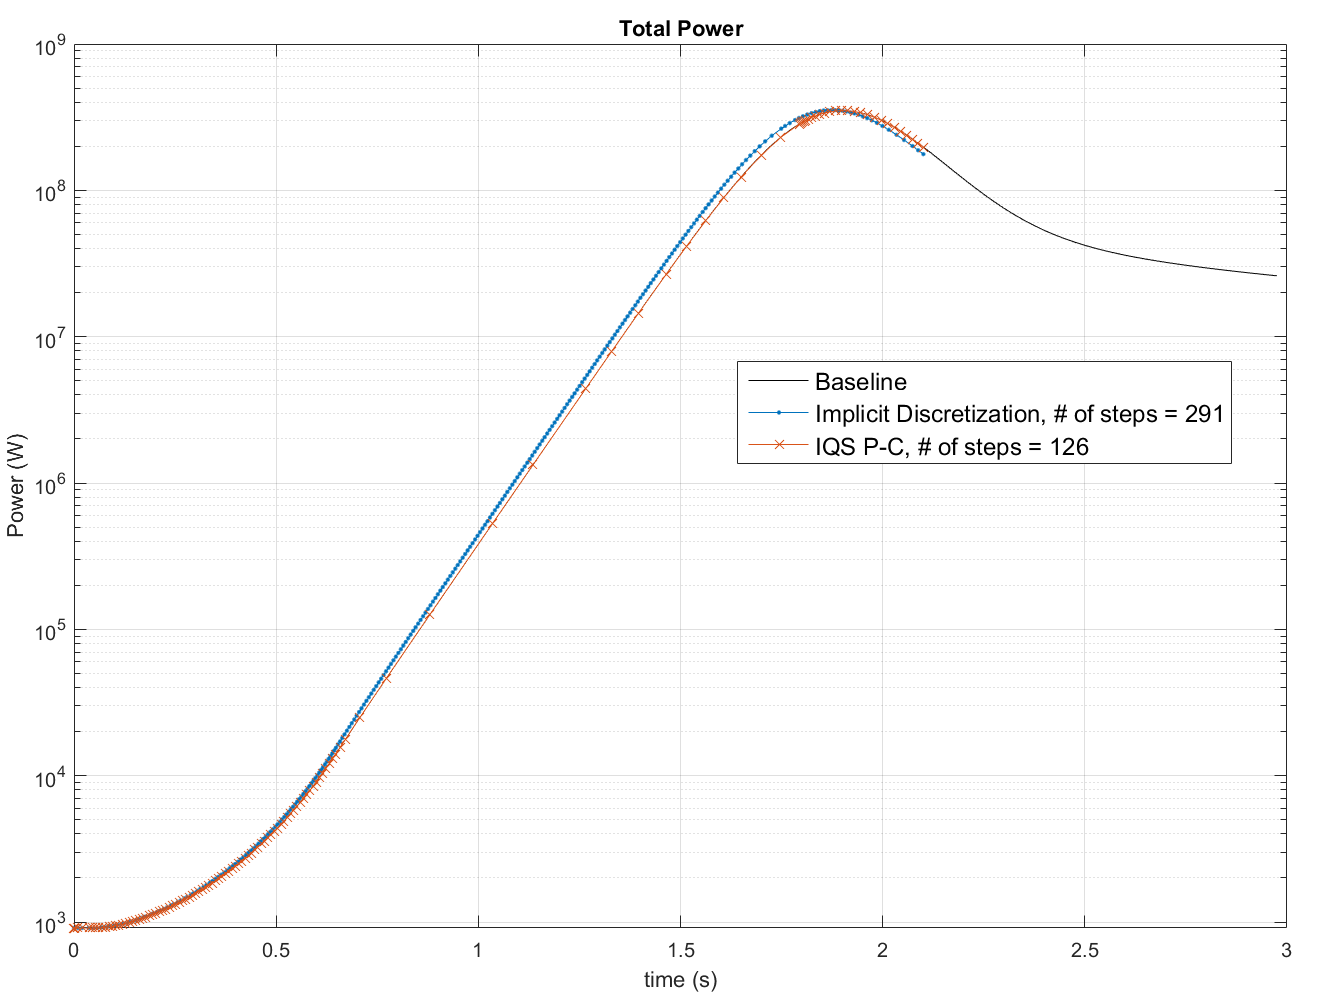
\includegraphics[width=\textwidth]{\FiguresDir/Tran15_DT2.png}
\caption{Full power profile}
\end{subfigure}
\begin{subfigure}[!htbp]{0.49\textwidth}
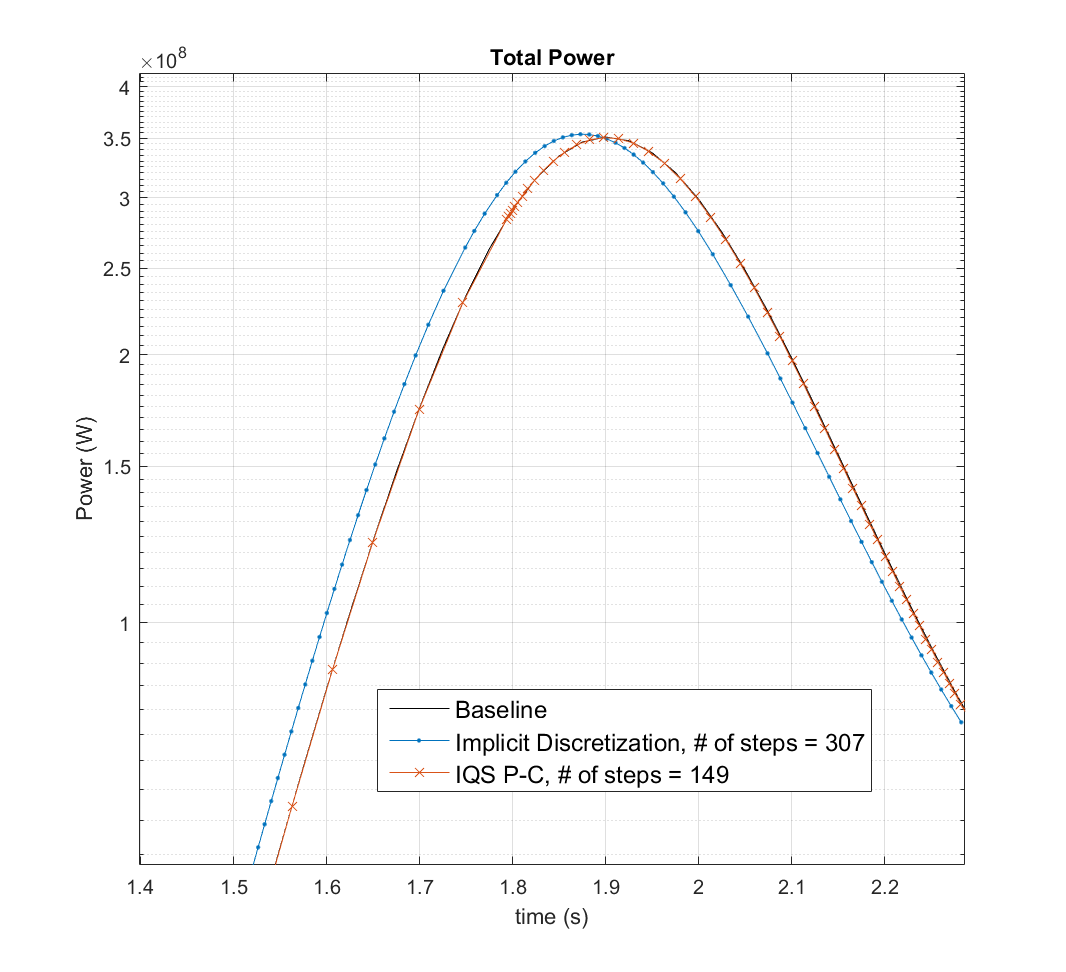
\includegraphics[width=\textwidth]{\FiguresDir/Tran15_DT2_peak.png}
\caption{Peak power profile}
\end{subfigure}
\caption{Transient-15 step doubling adaptation results with implicit discretization and IQS P-C}
\label{fig:Tran15_dt2}
\end{figure}

%\section{TREAT M8-CAL Problem}
%%%%%%%%%%%%%%%%%%%%%%%%%%%%%%%%%%%%%%%%%%%%%%%%%%%
%
%  New template code for TAMU Theses and Dissertations starting Fall 2016.
%
%  Author: Sean Zachary Roberson 
%	 Version 3.08.16
%  Last updated 8/19/2016
%
%%%%%%%%%%%%%%%%%%%%%%%%%%%%%%%%%%%%%%%%%%%%%%%%%%%

%%%%%%%%%%%%%%%%%%%%%%%%%%%%%%%%%%%%%%%%%%%%%%%%%%%%%%%%%%%%%%%%%%%%%%
%%                           SECTION IV
%%%%%%%%%%%%%%%%%%%%%%%%%%%%%%%%%%%%%%%%%%%%%%%%%%%%%%%%%%%%%%%%%%%%%

%%%%%%%%%%%%%%%%%%%%%%%%%%%%%%%%%%%%%%%%%%%%%%%%%%%%%%%%%%%%%%%%%%%%%
%%%%%%%%%%%%%%%%%%%%%%%%%%%%%%%%%%%%%%%%%%%%%%%%%%%%%%%%%%%%%%%%%%%%%
\chapter{\uppercase{Conclusions}}
%%%%%%%%%%%%%%%%%%%%%%%%%%%%%%%%%%%%%%%%%%%%%%%%%%%%%%%%%%%%%%%%%%%%%
%%%%%%%%%%%%%%%%%%%%%%%%%%%%%%%%%%%%%%%%%%%%%%%%%%%%%%%%%%%%%%%%%%%%%
\tcr{I am not sure but the present tense sounds weird when you conclude. How about a reformation as follows:
In this work, we analyzed/investigated ....}

The goal of this thesis research is to continue the investigation and development of the improved quasi-static method for the optimization of transient reactor simulations. In pursuit of this goal, three objectives are formulated: establish IQS behavior for various iteration techniques, validate time step convergence for IQS, and apply IQS to multiphysics simulations. The following three sections describe the purpose of each objective, as well as conclusions on their results. 

%%%%%%%%%%%%%%%%%%%%%%%%%%%%%%%%%%%%%%%%%%%%%%%%%%%%%%%%%%%%%%%%%%%%%
\section{Iteration Convergence Analysis}
%%%%%%%%%%%%%%%%%%%%%%%%%%%%%%%%%%%%%%%%%%%%%%%%%%%%%%%%%%%%%%%%%%%%%

IQS is a nonlinear system of equations; therefore, either fixed-point or Newton iteration is needed to evaluate shape and amplitude. Through literary review, most IQS applications used fixed-point iteration with various convergence criteria. Previous application of the Newton method is not discussed in detail, nor is any analysis of its convergence presented. Investigating these iteration techniques is important for understanding the behavior of IQS, as well as determining the most appropriate technique for optimal performance. The iteration techniques were applied to a one-dimensional prototype problem for testing. For fixed-point iteration, five different criteria were tested: 

\begin{enumerate}
\item $L^\infty$ norm of the change in shape between iterations
\item $L^2$ norm of the change in shape between iterations
\item Difference in reactivity between iterations
\item Difference in amplitude between iterations
\item IQS uniqueness consistency criteria
\end{enumerate}

The results showed that criteria 1-4 had relatively equivalent convergence behavior. However, iteration with the criteria 5 could not converge without a highly-accurate analytical treatment of the precursor equation. This criteria proved to be the most rigorous and thorough convergence criteria and is recommended for any application of IQS.

%%%%%%%%%%%%%%%%%%%%%%%%%%%%%%%%%%%%%%%%%%%%%%%%%%%%%%%%%%%%%%%%%%%%%
\section{Time Step Convergence Analysis}
%%%%%%%%%%%%%%%%%%%%%%%%%%%%%%%%%%%%%%%%%%%%%%%%%%%%%%%%%%%%%%%%%%%%%

Time step convergence analysis involves evaluating a problem with various refinements in step size and comparing the resulting errors with the time step size. Plotting error versus $\Delta t$ on a log-scale should produce a relatively strait line with a slope equal to the order of the time discretization method. \tcr{you are describing how to visualize convergence order. This should not be said here, in the conclusions, but before.}
Validating IQS by demonstrating proper error convergence is essential for predicting model error and using time adaptation techniques. Implicit Euler and BDF discretization schemes were applied to the one-dimensional prototype problem. IQS showed proper error convergence up through fourth order BDF schemes. Implicit Euler and second order BDF schemes were applied to the TWIGL benchmark, where IQS showed proper error convergence. Step doubling adaptation was also applied to TWIGL, where IQS performed impressively, reducing the number of diffusion evaluations considerably. The Crank-Nicholson scheme was applied to the LRA benchmark with IQS. IQS again showed proper second order convergence and was able to reduce the number of diffusion evaluations with time adaptation by more than a factor of 6. The results of the TWIGL and LRA benchmarks proved that IQS is capable of proper convergence and time adaptation behavior for more complex problems.
\tcr{Popov may balk at the repeated use of proper, but that's ok. If he says nothing, we let it go.}

%%%%%%%%%%%%%%%%%%%%%%%%%%%%%%%%%%%%%%%%%%%%%%%%%%%%%%%%%%%%%%%%%%%%%
\section{IQS Application to Multiphysics}
%%%%%%%%%%%%%%%%%%%%%%%%%%%%%%%%%%%%%%%%%%%%%%%%%%%%%%%%%%%%%%%%%%%%%

Full transient reactor simulation requires the implementation of multiphysics solution methods. In order to test IQS with these types of simulations, it was implemented into the MOOSE/Rattlesnake framework and executed using MAMMOTH. The LRA benchmark and a full core TREAT model were evaluated as test cases for multiphysics treatment. These examples involve a adiabatic heat up of the fuel with Doppler broadening feedback of cross-sections. The evaluation of temperature was integrated in the quasi-static process by introducing an intermediate time scale for temperature and PRKE parameter evaluation. The results of the LRA benchmark showed that quasi-static approach to temperature greatly improved the accuracy for a given time step size. However, the increase in computation time due to the extra temperature evaluations was significant. Therefore, for this benchmark, IQS with one update and IQS P-C with four updates is optimal. The results of the TREAT example showed similar behavior, except the updates only produced a marginal increase in accuracy. These examples' results and the dynamical time scale analysis show that performing a variant number of updates during the transient could further improve the performance of this quasi-static process. In conclusion, IQS and the quasi-static treatment of temperature can drastically improve the computational efficiency for burdensome full transient reactor simulations.

%%%%%%%%%%%%%%%%%%%%%%%%%%%%%%%%%%%%%%%%%%%%%%%%%%%%%%%%%%%%%%%%%%%%%
\section{Recommendations for Further Research}
%%%%%%%%%%%%%%%%%%%%%%%%%%%%%%%%%%%%%%%%%%%%%%%%%%%%%%%%%%%%%%%%%%%%%

This research intended to investigate IQS performance for transient reactor simulation and develop means for maximizing computational efficiency for these simulations. Further improvement and testing of IQS can be done in the following areas:

\begin{enumerate}

\item This thesis only applied IQS to fuel temperature feedback models. It is recommended that IQS be applied and tested with other feedback mechanisms such as thermal hydraulic and structural feedback, especially within the quasi-static process.

\item Application of IQS to neutron transport was hinted at in \sct{sect:transport}, but diffusion is typically sufficient for reactor simulation. It is recommended that IQS be applied to neutron transport with multiphysics and tested to see if similar performance is observed.

\item The large systems of full reactor models require a linear iteration process, such as GMRES, to evaluate efficiently. These processes usually implement a preconditioner to minimize the number of linear iterations and improve computation time. Investigating of an optimal preconditioner would \tcr{further} improve IQS performance in terms of computational efficiency.
\tcr{this reminds me that you may want to describe a bit the types of linear solution techniques (and their associated preconditioners) used when employing Rattlesnake. This is missing from the document I believe}

\end{enumerate}

\bibliographystyle{ieeetr}
\renewcommand{\bibname}{{\normalsize\rm REFERENCES}}
\bibliography{data/references_IQS}

%%%%%%%%%%%%%%%%%%%%%%%%%%%%%%%%%%%%%%%%%%%%%%%%%%%
%
%  New template code for TAMU Theses and Dissertations starting Fall 2016.  
%
%
%  Author: Sean Zachary Roberson 
%	 Version 3.16.09
%  Last updated 9/12/2016
%
%%%%%%%%%%%%%%%%%%%%%%%%%%%%%%%%%%%%%%%%%%%%%%%%%%%

\begin{appendices}
\titleformat{\chapter}{\centering\normalsize}{APPENDIX \thechapter}{0em}{\vskip .5\baselineskip\centering}
\renewcommand{\appendixname}{APPENDIX}

%%%%%%%%%%%%%%%%%%%%%%%%%%%%%%%%%%%%%%%%%%%%%%%%%%%
%
%  New template code for TAMU Theses and Dissertations starting Fall 2016.
%
%
%  Author: Sean Zachary Roberson 
%	 Version 3.16.09
%  Last updated 9/12/2016
%
%%%%%%%%%%%%%%%%%%%%%%%%%%%%%%%%%%%%%%%%%%%%%%%%%%%

%%%%%%%%%%%%%%%%%%%%%%%%%%%%%%%%%%%%%%%%%%%%%%%%%%%%%%%%%%%%%%%%%%%%%%
%%                           APPENDIX A 
%%%%%%%%%%%%%%%%%%%%%%%%%%%%%%%%%%%%%%%%%%%%%%%%%%%%%%%%%%%%%%%%%%%%%

\phantomsection

\chapter{\uppercase{Derivations}}

%%---------------------------------------------------------------------------%%
\section{Derivation of IQS with CFEM Diffusion}
%%---------------------------------------------------------------------------%%

Multigroup diffusion equation with delayed neutron precrusors:
\begin{align}
\frac{\partial}{\partial t}\left(\frac{\phi^g}{v^g}\right) =& \chi_p^g \sum_{g'=1}^G (1-\beta) \frac{\nu^{g'} \Sigma_f^{g'}}{\keff} \phi^{g'} -  \left( -\div D^g \grad  + \Sigma_r^g \right) \phi^g  \nonumber \\
&  + \sum_{g'\neq g}^G\Sigma_s^{g'\to g} \phi^{g'}  + \sum_{i=1}^I\chi_{d,i}^g\lambda_i C_i \ , \quad 1 \le g \le G 
\label{eq:diffusion}
\end{align}
\be
\frac{dC_i}{dt} = \beta_i\sum_{g=1}^G \frac{\nu^{g'} \Sigma_f^{g'}}{\keff} \phi^{g} - \lambda_i C_i \ , \quad 1 \le i \le I 
\label{eq:precA}
\ee

With reflecting and vacuum boundary conditions:
\be 
\begin{cases} 
\grad\phi^g = 0, &\vr\in\partial\D_2 \\ D\grad\phi^g-\frac{1}{2}\phi^g = 0, &\vr\in\partial\D_3
\end{cases}
\ee
\be 
\text{with } \partial\D=\partial\D_2\cup\partial\D_3 \nonumber
\ee

Multiplying Equation~\ref{eq:diffusion} by the adjoint solution $\phi^{*g}$ and Equation~\ref{eq:precA} by $C^*=\sum_{g=1}^G\phi^{*g} \chi_{d,i}^g$ for test functions and integrating in space:
\begin{align}
&\frac{d}{dt}\left(\phi^{*g},\frac{1}{v^g}\phi^g\right)_\D = \left(\phi^{*g}\chi_p^g(1-\beta),\sum_{g'=1}^G \frac{\nu^{g'} \Sigma_f^{g'}}{\keff} \phi^{g'}\right)_\D + \left(\grad \phi^{*g},D^g \grad \phi^g\right)_\D \nonumber \\
& - \frac{1}{2}\left\langle\phi^{*g},\phi^{g}\right\rangle_{\partial \D_3} - \left(\phi^{*g},\Sigma_r^g\phi^g\right)_\D + \sum_{g'\neq g}^G\left(\phi^{*g},\Sigma_s^{g'\to g} \phi^{g'}\right)_\D + \sum_{i=1}^I \left(\phi^{*g}\chi_{d,i}^g,\lambda_i C_i\right)_\D
\label{eq:diffweak}
\end{align}
\be
\frac{d}{dt}\left(C^*,C_i\right)_\D = \left(C^* \beta_i,\sum_{g'=1}^G\frac{\nu^{g'} \Sigma_f^{g'}}{\keff}\varphi^{g'}\right)_\D -\left(C^*,\lambda_i C_i\right)_\D
\ee

Summing over groups on both sides of Equation~\ref{eq:diffweak}:
\begin{align}
\frac{d}{dt}&\left(\sum_{g=1}^G\left(\phi^{*g},\frac{1}{v^g}\phi^g\right)_\D\right) = \left(\sum_{g=1}^G\phi^{*g}\chi_p^g(1-\beta),\sum_{g'=1}^G \frac{\nu^{g'} \Sigma_f^{g'}}{\keff} \phi^{g'}\right)_\D  \nonumber \\ 
& + \sum_{g=1}^G\left(\grad \phi^{*g},D^g \grad \phi^g\right)_\D - \frac{1}{2}\sum_{g=1}^G\left\langle\phi^{*g},\phi^{g}\right\rangle_{\partial \D_3} - \sum_{g=1}^G\left(\phi^{*g},\Sigma_r^g\phi^g\right)_\D  \nonumber \\ 
&+ \sum_{g=1}^G\sum_{g'\neq g}^G\left(\phi^{*g},\Sigma_s^{g'\to g} \phi^{g'}\right)_\D + \sum_{i=1}^I \left(\sum_{g=1}^G\phi^{*g}\chi_{d,i}^g,\lambda_i C_i\right)_\D 
\end{align}

Defining bilinear functions:
\begin{align}
T(\phi^{*},\phi) =& \sum_{g=1}^G\left(\phi^{*g},\frac{1}{v^g}\phi^g\right)_\D \\
C_i(C^*,C_i) =& \left(C^*,C_i\right)_\D \\
F(\phi^{*},\phi) =& \left(\sum_{g=1}^G\phi^{*g}\left(\chi_p^g(1-\beta)+\sum_{i=1}^I\chi_{d,i}^g\beta_i\right),\sum_{g'=1}^G \frac{\nu^{g'} \Sigma_f^{g'}}{\keff} \phi^{g'}\right)_\D \\
L(\phi^{*},\phi) =& \sum_{g=1}^G\left(-\left(\grad \phi^{*g},D^g \grad \phi^g\right)_\D + \frac{1}{2}\left\langle\phi^{*g},\phi^{g}\right\rangle_{\partial \D_3} + \left(\phi^{*g},\Sigma_r^g\phi^g\right)_\D \right) \\
S(\phi^{*},\phi) =& \sum_{g=1}^G\sum_{g'\neq g}^G\left(\phi^{*g},\Sigma_s^{g'\to g} \phi^{g'}\right)_\D \\
F_{d,i}(\phi^*,\phi) =& \left(\beta_i\sum_{g=1}^G\phi^{*g} \chi_{d,i}^g,\sum_{g'=1}^G\frac{\nu^{g'} \Sigma_f^{g'}}{\keff}\phi^{g'}\right)_\D \\
S_{d,i}(\phi^*,\phi) =& \left(\sum_{g=1}^G\phi^{*g} \chi_{d,i}^g,\lambda_i C_i\right)_\D \\
P_i(C^*,\phi) =& \left(C^*\beta_i,\sum_{g'=1}^G\frac{\nu^{g'} \Sigma_f^{g'}}{\keff}\phi^{g'}\right)_\D \\
D_i(C^*,C_i) =& \left(C^*,\lambda_i C_i\right)_\D
\end{align}

Rewriting the flux and precursor equations:
\be
\frac{d}{dt} T(\phi^{*},\phi) = F(\phi^{*},\phi) - \sum_{i=1}^I F_{d,i}(\phi^*,\phi) - L(\phi^{*},\phi) + S(\phi^{*},\phi) + \sum_{i=1}^I S_{d,i}(\phi^*,\phi)
\ee
\be
\frac{d}{dt} C_i(C^*,C_i) = P_i(C^*,\phi) - D_i(C^*,C_i)
\ee

Doing IQS factorization:
\begin{align}
\frac{d}{dt} T(\phi^{*},\varphi) = F(\phi^{*},\varphi) - \sum_{i=1}^I F_{d,i}(\phi^*,\varphi) &- L(\phi^{*},\varphi) - \frac{1}{p}\frac{dp}{dt}T(\phi^{*},\varphi) \nonumber \\
& + S(\phi^{*},\varphi) + \frac{1}{p}\sum_{i=1}^I S_{d,i}(\phi^*,\phi)
\end{align}
\be
\frac{\partial}{\partial t} C_i(C^*,C_i) = P_i(C^*,\varphi)p - D_i(C^*,C_i)
\ee

Defining PRKE parameters:
\be
\rho = \frac{F(\phi^{*},\varphi) - L(\phi^{*},\varphi) + S(\phi^{*},\varphi)}{F(\phi^{*},\varphi)}
\ee
\be
\bar{\beta} = \sum_{i=1}^I\bar{\beta}_i = \sum_{i=1}^I\frac{F_{d,i}(\phi^*,\varphi)}{F(\phi^{*},\varphi)} = \sum_{i=1}^I\frac{P_i(C^*,\varphi)}{F(\phi^{*},\varphi)}
\ee
\be
\Lambda = \frac{T(\phi^{*},\varphi)}{F(\phi^{*},\varphi)}
\ee
\be
\bar{\lambda}_i = \frac{S_{d,i}(\phi^*,\varphi)}{C_i(C^*,C_i)} = \frac{D_i(C^*,C_i)}{C_i(C^*,C_i)}
\ee
\be
\xi_i = \frac{C_i(C^*,C_i)}{T(\phi^{*},\varphi)}
\ee

Writing implementing parameters:
\be
\frac{dp}{dt}=\left[\frac{\rho-\bar{\beta}}{\Lambda}\right]p + \sum_{i=1}^I\bar{\lambda}_i\xi_i + p\frac{1}{T(\phi^{*},\varphi)}\frac{\partial}{\partial t} T(\phi^{*},\varphi)
\ee
\be
\frac{d\xi_i}{dt}=\frac{\bar{\beta}_i}{\Lambda}p-\bar{\lambda}_i\xi_i \quad 1 \le i \le I 
\ee

Assuming $\frac{\partial}{\partial t} T(\phi^{*},\varphi) = 0$:
\be
\frac{dp}{dt}=\left[\frac{\rho-\bar{\beta}}{\Lambda}\right]p+\sum_{i=1}^I\bar{\lambda}_i\xi_i
\label{eq:p}
\ee
\be
\frac{d\xi_i}{dt}=\frac{\bar{\beta}_i}{\Lambda}p-\bar{\lambda}_i\xi_i \quad 1 \le i \le I 
\label{eq:xi}
\ee

%%---------------------------------------------------------------------------%%
\section{Proof of Flux-Shape Solution Inequality}
%%---------------------------------------------------------------------------%%

There has been a reoccurring question that if shape and amplitude have same time step and integration scheme, the solution should be equal to the full flux solution.  This section is meant to prove that this notion is not true.  For simplicity, the integration scheme chosen was backward-Euler.  Writing the shape equation in time discretized form:

\begin{align}
&\frac{T^{n+1}(\phi^{*},\varphi)-T^{n}(\phi^{*},\varphi)}{\Delta t} = F^{n+1}(\phi^{*},\varphi) - \sum_{i=1}^I F_{d,i}^{n+1}(\phi^{*},\varphi) - L^{n+1}(\phi^{*},\varphi) -  \nonumber \\
&- \frac{1}{p^{n+1}}\frac{p^{n+1} - p^n}{\Delta t}T^{n+1}(\phi^{*},\varphi) + S^{n+1}(\phi^{*},\varphi) + \frac{1}{p^{n+1}}\sum_{i=1}^I S_{d,i}^{n+1}(\phi^{*},C_i)
\end{align}

where $n$ is the index for the previous time step and $n+1$ is the next one.  Multiplying both sides by $p^{n+1}$:
\begin{align}
&p^{n+1}\frac{T^{n+1}(\phi^{*},\varphi)-T^{n}(\phi^{*},\varphi)}{\Delta t} = F^{n+1}(\phi^{*},\varphi)p^{n+1} - \sum_{i=1}^I F_{d,i}^{n+1}(\phi^{*},\varphi)p^{n+1} \nonumber \\
& - L^{n+1}(\phi^{*},\varphi)p^{n+1} - \frac{p^{n+1} - p^n}{\Delta t}T^{n+1}(\phi^{*},\varphi) + S^{n+1}(\phi^{*},\varphi)p^{n+1} + \sum_{i=1}^I S_{d,i}^{n+1}(\phi^{*},C_i)
\end{align}

Notice that for any bilinear form with $\varphi$, when multiplied by $p^{n+1}$ is the same form, but with $\phi$ instead. So:
\begin{align}
p^{n+1}&\frac{T^{n+1}(\phi^{*},\varphi)-T^{n}(\phi^{*},\varphi)}{\Delta t} + \frac{p^{n+1} - p^n}{\Delta t}T^{n+1}(\phi^{*},\varphi)= F^{n+1}(\phi^{*},\phi)  \nonumber \\
&- \sum_{i=1}^I F_{d,i}^{n+1}(\phi^{*},\phi) - L^{n+1}(\phi^{*},\phi) + S^{n+1}(\phi^{*},\phi) + \sum_{i=1}^I S_{d,i}^{n+1}(\phi^{*},C_i)
\label{eq:dshape}
\end{align}

Now the full flux equation is discretized the same way:
\begin{align}
\frac{T^{n+1}(\phi^{*},\phi)-T^{n}(\phi^{*},\phi)}{\Delta t} =& F^{n+1}(\phi^{*},\phi)- \sum_{i=1}^I F_{d,i}^{n+1}(\phi^{*},\phi) \nonumber \\
& - L^{n+1}(\phi^{*},\phi) + S^{n+1}(\phi^{*},\phi) + \sum_{i=1}^I S_{d,i}^{n+1}(\phi^{*},C_i)
\label{eq:dflux}
\end{align}

Notice that Equations~\ref{eq:dshape}~and~\ref{eq:dflux} have the same right hand side. So the left hand side of each equation can be equated, while converting the left hand side of Equation \ref{eq:dflux} to amplitude and flux:

\begin{align}
\frac{p^{n+1}T^{n+1}(\phi^{*},\varphi)-p^nT^{n}(\phi^{*},\varphi)}{\Delta t} &= p^{n+1}\frac{T^{n+1}(\phi^{*},\varphi)-T^{n}(\phi^{*},\varphi)}{\Delta t} \nonumber \\
&+ \frac{p^{n+1} - p^n}{\Delta t}T^{n+1}(\phi^{*},\varphi)
\label{eq:neq}
\end{align}

From Equation~\ref{eq:p}:
\be
\frac{p^{n+1} - p^n}{\Delta t} = \left[\frac{\rho^{n+1}-\bar{\beta}^{n+1}}{\Lambda^{n+1}}\right]p^{n+1}+\sum_{i=1}^I\bar{\lambda}_i^{n+1}\xi_i^{n+1}
\ee

Substituting the PRKE parameter definitions:
\begin{align}
\frac{p^{n+1} - p^n}{\Delta t} T^{n+1}(\phi^{*},\varphi) =& F^{n+1}(\phi^{*},\phi)- \sum_{i=1}^I F_{d,i}^{n+1}(\phi^{*},\phi) \nonumber \\
& - L^{n+1}(\phi^{*},\phi) + S^{n+1}(\phi^{*},\phi) + \sum_{i=1}^I S_{d,i}^{n+1}(\phi^{*},C_i)
\label{eq:dprke}
\end{align}

Notice how the right hand side of Equation~\ref{eq:dprke} is equal to the right hand side of Equation~\ref{eq:dflux} so:
\be
\frac{p^{n+1} - p^n}{\Delta t} T^{n+1}(\phi^{*},\varphi) = \frac{p^{n+1}T^{n+1}(\phi^{*},\varphi)-p^nT^{n}(\phi^{*},\varphi)}{\Delta t}
\ee

Substituting this into the last term on the right hand side of Equation~\ref{eq:neq}:

\begin{align}
\frac{p^{n+1}T^{n+1}(\phi^{*},\varphi)-p^nT^{n}(\phi^{*},\varphi)}{\Delta t} &= p^{n+1}\frac{T^{n+1}(\phi^{*},\varphi)-T^{n}(\phi^{*},\varphi)}{\Delta t} \nonumber \\
&+ \frac{p^{n+1}T^{n+1}(\phi^{*},\varphi)-p^nT^{n}(\phi^{*},\varphi)}{\Delta t}
\label{eq:neq2}
\end{align}

Which can be written as:
\be
\frac{T^{n+1}(\phi^{*},\varphi)-T^{n}(\phi^{*},\varphi)}{\Delta t} = 0
\ee

 However, this equation is not necessarily true.  The assumption is made that $\frac{dT}{dt} = 0$ when deriving Equation~\ref{eq:p}, but in practice this doesn't always hold up. Therefore, putting the shape and amplitude equations on the same discretization, does not necessarily mean the IQS solution will produce the same solution as the full flux equation.
 
To show this result numerically, the discretized scheme was applied to the one-group, one-dimensional example and five Picard iterations were done each time step for IQS.  The compiled results are shown in Table \ref{tab:neq} by comparing the difference in the volumetric integral of the flux. The results show that there is an average 1\% difference between the full flux solution and IQS.

%\begin{table}
%\centering
%\caption{Numerical results for inequality proof where the compared value is $(1,\phi)$}
%\label{tab:neq}
%\begin{tabular}{llll}
%\csvautotabular{\FiguresDir/inequality_results.csv}
%\end{tabular}
%\end{table}

\begin{table}
\centering
\caption{Numerical results for inequality proof where the compared value is $(1,\phi)$}
\label{tab:neq}
\begin{tabular}{|llll|}
\hline
Time(s) &	Full Flux Solve &	IQS Solve &	Relative Difference \\
\hline
0.0	&	0.90903993 &	0.90903993 &	0		\\
0.1 &	0.91253395 &	0.90903993 &	0.00383 \\
0.2 &	0.92068212 &	0.91341921 &	0.00789 \\
0.3 &	0.93564944 &	0.92419479 &	0.01224 \\
0.4 &	0.96072564 &	0.94502984 &	0.01634 \\
0.5 &	1.00132530 &	0.98193047 &	0.01937 \\
0.6 &	1.06731452 &	1.04589052 &	0.02007 \\
0.7 &	1.13375988 &	1.11085442 &	0.0202 \\
0.8 &	1.19865931 &	1.17468271 &	0.02 \\
0.9 &	1.26133943 &	1.23659429 &	0.01962 \\
1.0 &	1.32173672 &	1.29643586 &	0.01914 \\
1.1 &	1.33970601 &	1.31604696 &	0.01766 \\
1.2 &	1.32132462 &	1.30051903 &	0.01575 \\
1.3 &	1.27831729 &	1.26067046 &	0.0138 \\
1.4 &	1.22290272 &	1.20822518 &	0.012 \\
1.5 &	1.16481963 &	1.15274011 &	0.01037 \\
1.6 &	1.11035980 &	1.10047097 &	0.00891 \\
1.7 &	1.06269788 &	1.05460529 &	0.00762 \\
1.8 &	1.03149816 &	1.02465437 &	0.00663 \\
1.9 &	1.01107465 &	1.00511526 &	0.00589 \\
2.0 &	0.99776339 &	0.99243083 &	0.00534 \\
\hline
\end{tabular}
\end{table}
%%%%%%%%%%%%%%%%%%%%%%%%%%%%%%%%%%%%%%%%%%%%%%%%%%%
%
%  New template code for TAMU Theses and Dissertations starting Fall 2016.
%
%
%  Author: Sean Zachary Roberson 
%	 Version 3.16.09 
%  Last updated 9/12/2016
%
%%%%%%%%%%%%%%%%%%%%%%%%%%%%%%%%%%%%%%%%%%%%%%%%%%%

%%%%%%%%%%%%%%%%%%%%%%%%%%%%%%%%%%%%%%%%%%%%%%%%%%%%%%%%%%%%%%%%%%%%%%
%%                           APPENDIX B
%%%%%%%%%%%%%%%%%%%%%%%%%%%%%%%%%%%%%%%%%%%%%%%%%%%%%%%%%%%%%%%%%%%%%

\chapter{\uppercase {Other Testing}}


\section{SDIRK Convergence Problems}

In order to figure what is causing convergence problems for SDIRK, a manufactured solution was created in the one-dimensional prototype code, described by \eqt{eq:mms}. A second order finite element basis function was used, so the spatial profile was known exactly with only one degree of freedom. The ODE describing this degree of freedom is shown by \eqt{eq:mms_ode}. The coefficients represented in this equation are defined by \eqt{eq:mms_coef}.

\be 
\phi(x,t) = x(1-x)(1+t)^4 \qq 0 \leq x \leq 1
\label{eq:mms}
\ee
\be 
\frac{1}{v}\frac{\partial\phi}{\partial t} = \alpha\phi + \frac{\beta}{v}4(1+t)^3 + \gamma(1+t)^4
\label{eq:mms_ode}
\ee


\begin{subequations}
\be 
\alpha = -D\int_0^1 (4(1-2x))^2dx + (\nu\Sigma_f-\Sigma_a)\int_0^1 (4x(1-x))^2dx = -5.28
\ee
\be 
\beta = \frac{1}{4}\int_0^1(4x(1-x))^2dx = 0.1333
\ee
\be 
\gamma = (\Sigma_a-\nu\Sigma_f)\beta+2D\int_0^1 4x(1-x)dx = 1.32
\ee
\label{eq:mms_coef}
\end{subequations}

The ODE was then evaluated using SDIRK and BDF schemes with varying velocities. \fig{fig:mms1} compares SDIRK and BDF convergence with a relatively large $v$. This plot shows the SDIRK is unable to establish a proper error convergence for such a stiff problem. \fig{fig:mms2} compares SDIRK convergence lines with different velocities. This plot shows that only at relatively small values of $v$, is SDIRK able to show proper convergence.

\begin{figure}[htpb!]
\centering
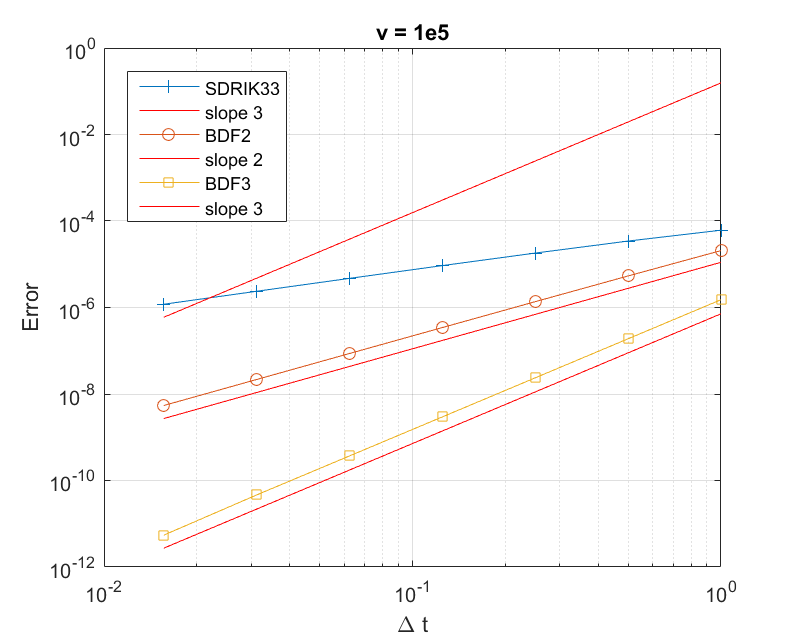
\includegraphics[width=\linewidth]{\FiguresDir/sdirk_mms1.png}
\caption{SDIRK33 vs. BDF convergence with $v=1e5$}
\label{fig:mms1}
\end{figure}

\begin{figure}[htpb!]
\centering
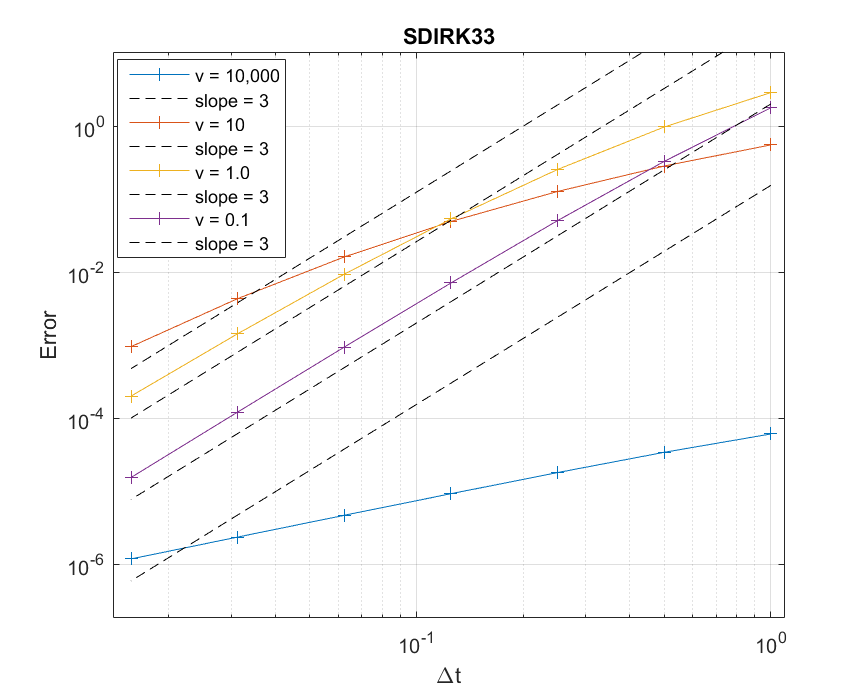
\includegraphics[width=\linewidth]{\FiguresDir/sdirk_mms2.png}
\caption{SDIRK33 convergence with different velocities}
\label{fig:mms2}
\end{figure}

\pagebreak{}

\end{appendices}


\end{document}
